\documentclass[11pt,a4paper]{report}
\usepackage[utf8]{inputenc}
\usepackage[english]{babel}
\usepackage[toc,page]{appendix}
\usepackage{amsmath}
\usepackage{amsthm}
\usepackage{amsfonts}
\usepackage{amssymb}
\usepackage{color}
\usepackage[a4paper]{geometry}
\usepackage{listings}
\usepackage{minted}
\usepackage{float}
\usepackage[table]{xcolor}
\usepackage{dirtytalk}
\UseRawInputEncoding
\usepackage{graphicx}
\usepackage{caption}
\usepackage{subcaption}
\usepackage{array}
\usepackage{multirow}
\usepackage{mathtools}
\usepackage{dsfont}
\usepackage[thinc]{esdiff}
\usepackage{tocbibind}
\usepackage{parskip}
\usepackage[ruled,vlined]{algorithm2e}
\DeclareMathOperator*{\argminB}{argmin}
\DeclareMathOperator*{\argmaxB}{argmax}
\DeclareMathOperator{\EX}{\mathbb{E}}
\newtheorem{theorem}{Theorem}
\newtheorem{definition}{Definition}
\graphicspath{ {./images/} }


\title{Statistical Machine Learning using Tree-Based Methods}
\author{Pattanin (Mill) Luangamornlert}
\date{\today}

\pagenumbering{roman}
\begin{document}
\maketitle

\begin{abstract}
    \emph{This piece of work is a result of my own work except where it forms an assessment based on group project work. In the case of a group project, the work has been prepared in collaboration with other members of the group. Material from the work of others not involved in the project has been acknowledged and quotations and paraphrases suitably indicated.}
    \bigskip
    
    This project aims to look at methods of Machine Learning, which has been described as the 4th Industrial Revolution (4IR) by the World Economic Forum at Davos in 2016 \cite{Schwab}.
    
    We will look at the mathematics behind Decision Trees, famously described in Leo Breiman's landmark book Classification and Regression Trees \cite{BreimanDT} which is one of the most cited sources for Statistical Machine Learning, with over 48,000 citations.
    
    Breiman, Friedman, Olshen, and Stone noted that CART had its flaws in the book itself and have always strived to improve the method, Breiman introducing Random Forests a few years later, and Friedman created Gradient Boosted Machines in 1999. Since then, many mathematicians have tried to improve upon the work and this project will try to explore these methods.
    \bigskip\\
    \textbf{Key Words:} Classification, Regression, Decision Trees, Metrics, Bootstrap, Optimization, Interpretability,
    
    
    
\end{abstract}




\tableofcontents
\listofalgorithms
\listoffigures


\chapter{An Introduction to Machine Learning}
\pagenumbering{arabic}
Machine Learning is a subset of Artificial Intelligence (AI) where we create a mathematical model which can be ``trained" using previously known data to create a more robust AI programme which can be deployed in the real world.
We achieve this by using Statistics to create models which we then feed into the machine for it to predict outcomes based on prior events.


\section{Supervised and Unsupervised Learning}
In statistics, there are two objectives which become possible when you look at a data set.

\begin{itemize}
  \item \textbf{Supervised Learning} where we observe how $X$ affects $Y$ as we change the variable $X$
  
  \item \textbf{Unsupervised Learning} we investigate the characteristics of $X$ and how it behaves relative to the rest of the data
\end{itemize}
The methods we will explore will be a Supervised Learning method.\\
There are two main ways to deal with data under Supervised Learning:
\begin{itemize}
    \item \textbf{Classification} - classification is suited when you want to group data together to make predictions which are quantitative. 
    Methods include: Logistic Regression, Support Vector Machines etc.
    
    \item \textbf{Regression} - Regression is the main form of statistical analysis for continuous forms of data as they can be used to build a trend line to estimate an output $Y$ from $X$ based on previously known information.
    Methods include: Linear Regression
\end{itemize}
To see how these work, please consult the following books.
\begin{enumerate}
    \item \textbf{An Introduction to Statistical Learning} \cite[Chapter 3-4]{ISLR} 
    
    \item \textbf{Elements of Statistical Learning} \cite[Chapter 3-4]{ESL}
\end{enumerate}


\section{What are Decision Trees?}
\textbf{Decision Trees} are essentially a flow chart that is shaped like a tree which is used to make predictions. 
They are a form of non-parametric statistics and a common and easy to interpret alternative for when data is non-linear.
The aim is to input multiple variables (often historical data) into the model, and under supervised learning, we are able to predict the outcome of a future test using the same variables as in the test data.\\
Each decision point is called a ``Parent" node, where at each node, we split the set of data into root nodes - called ``Child" nodes.
This is done recursively until a stopping point has been achieved.
Decision Trees are used widely in industry, such as in medicine where a tree is often used to predict if a patient has cancer or not. 
\medskip\\
Decision Trees provide many advantages over other methods:
\begin{itemize}
    \item They are very easy to understand
    
    \item They do not require lots of effort with regards to data processing
    
    \item Data can be left as is - no normalization or scaling is needed
    
    \item Missing data can be ignored as they do not affect the learning of the model
\end{itemize}

\subsection{Basic History of Decision Trees \cite{50years}} 
The idea of Decision Trees first came out of Operations Research as an optimization problem. 
This was first developed in 1963 \cite{AID} and the method is called Automatic Interaction Detection (AID).
AID splits the model into subsets and does that recursively until a stopping criteria is met.
However, AID is a regression tree algorithm and so development for a classification naturally followed.
\medskip\\
This ended up being developed into Theta Automatic Interaction Detection (THAID) \cite{THAID}.
THAID splits data using classification methods but had its flaws and was superseded by Chi-square Automatic Interaction Detection (CHAID) \cite{CHAID}. 
In this case we split data into intervals and merge the groups which are not as significant together. From here, Bonferroni corrections are used.
\medskip\\
Unfortunately, this method was still not optimal and thus a better approach was needed.
Thus, the idea of metrics were introduced as a splitting criterion.

\subsection{The CART method - and where do we go on from it?}
Multiple algorithms can be used to create a Decision Tree. 
The most famous of these, Classification and Regression Trees (CART) \cite{BreimanDT} was the first developed by Leo Breiman, Jerome Friedman and others in the 1984 book, Classification and Regression Trees.
An alternative, ID3 by Ross Quinlan \cite{Quinlan}, was introduced in 1985 and uses similar ideas but with minor differences which will be discussed later.
It is another popular method and indeed, some may prefer it to CART while others may find its limitations too restrictive.
\medskip\\
Firstly, we will look at how the CART algorithm actually works and show some examples for both classification and regression problems. 
From here we are able to look at the multitude of methods which have been used to improve upon the CART method, such as Random Forest, Gradient Boosting and Optimal Decision Trees.

\subsubsection{A Basic Example of CART in action}
Here we have a graphical example of how CART is used on the Penguins Dataset \cite{penguins} to classify penguin species:
\begin{figure}[H]
    \centering
    \begin{subfigure}[b]{0.4\textwidth}
        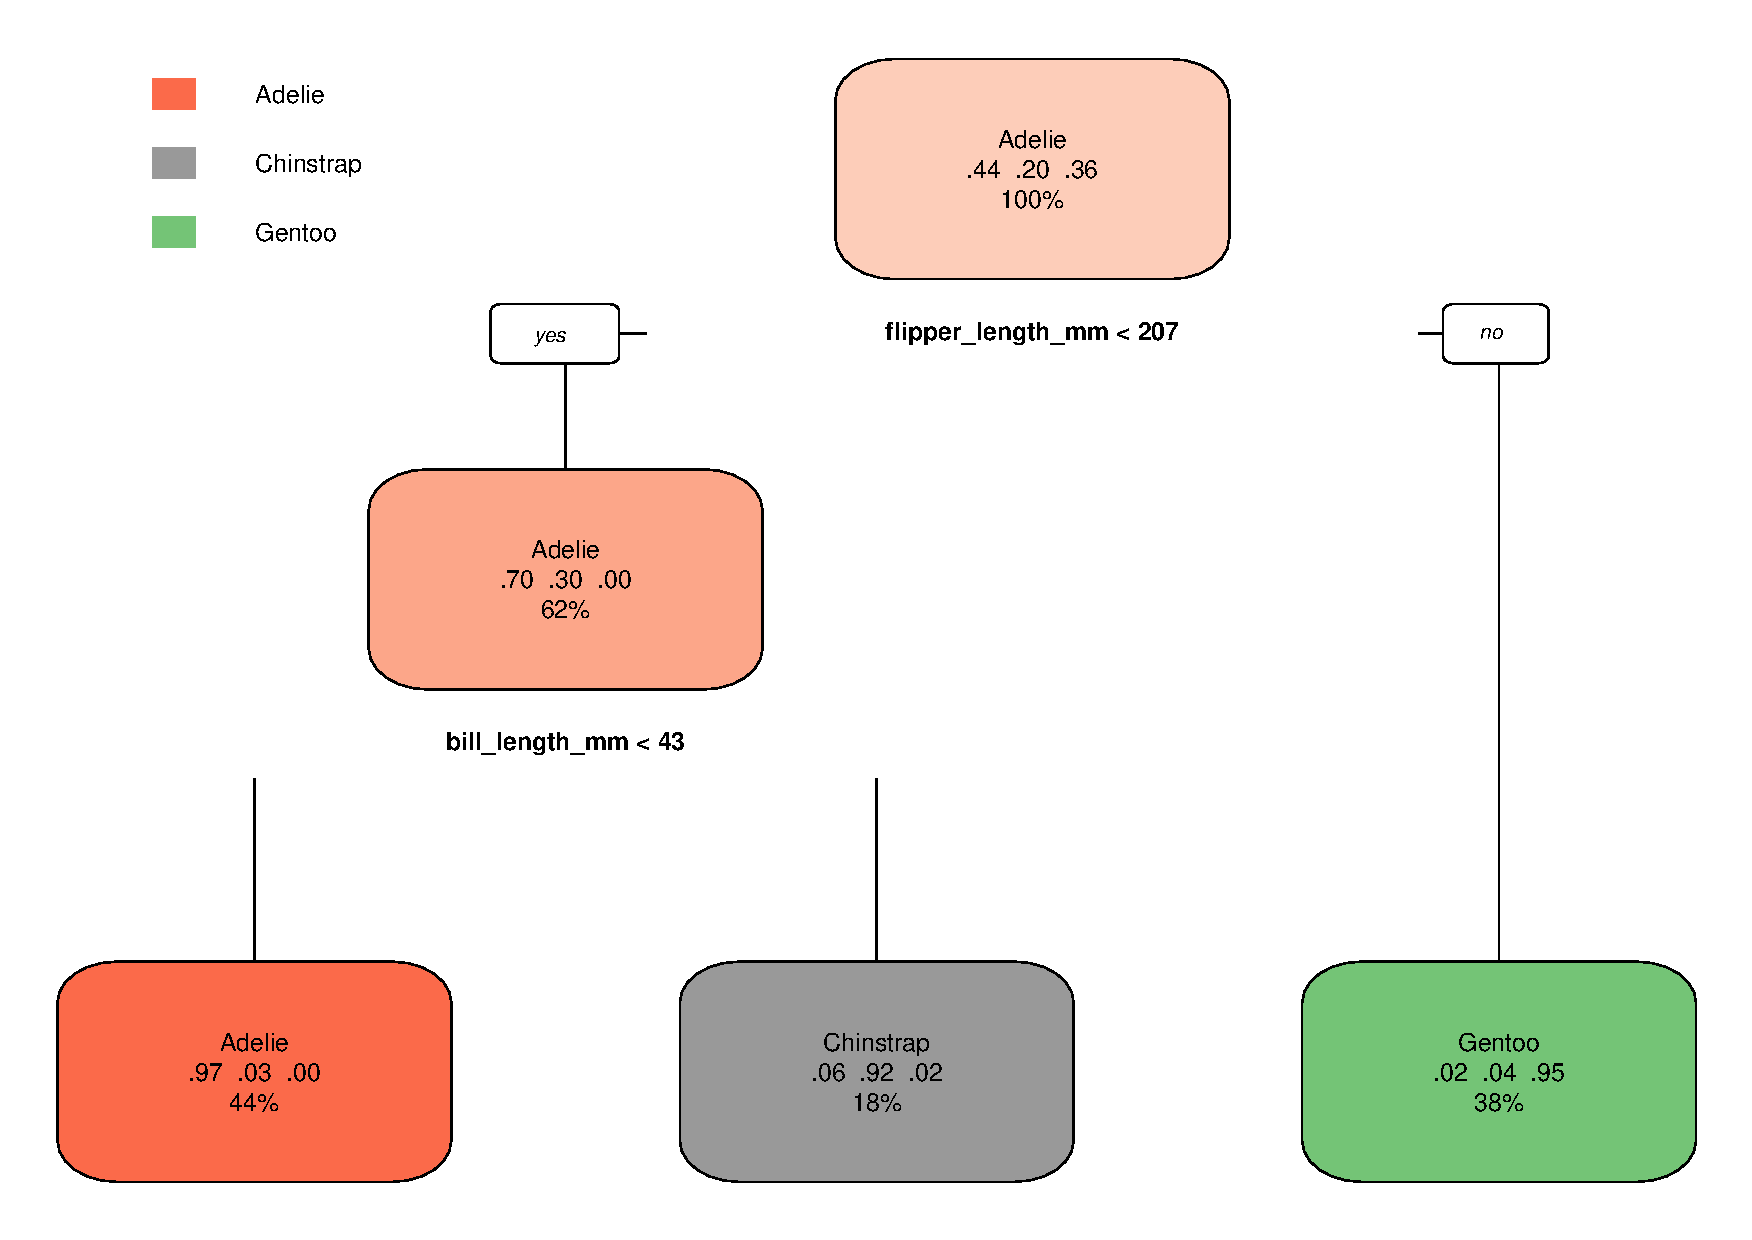
\includegraphics[width=\textwidth]{presentation/Penguintree.pdf}
        \caption{Classification Tree}
        \label{fig:pentree}
    \end{subfigure}
    \begin{subfigure}[b]{0.4\textwidth}
        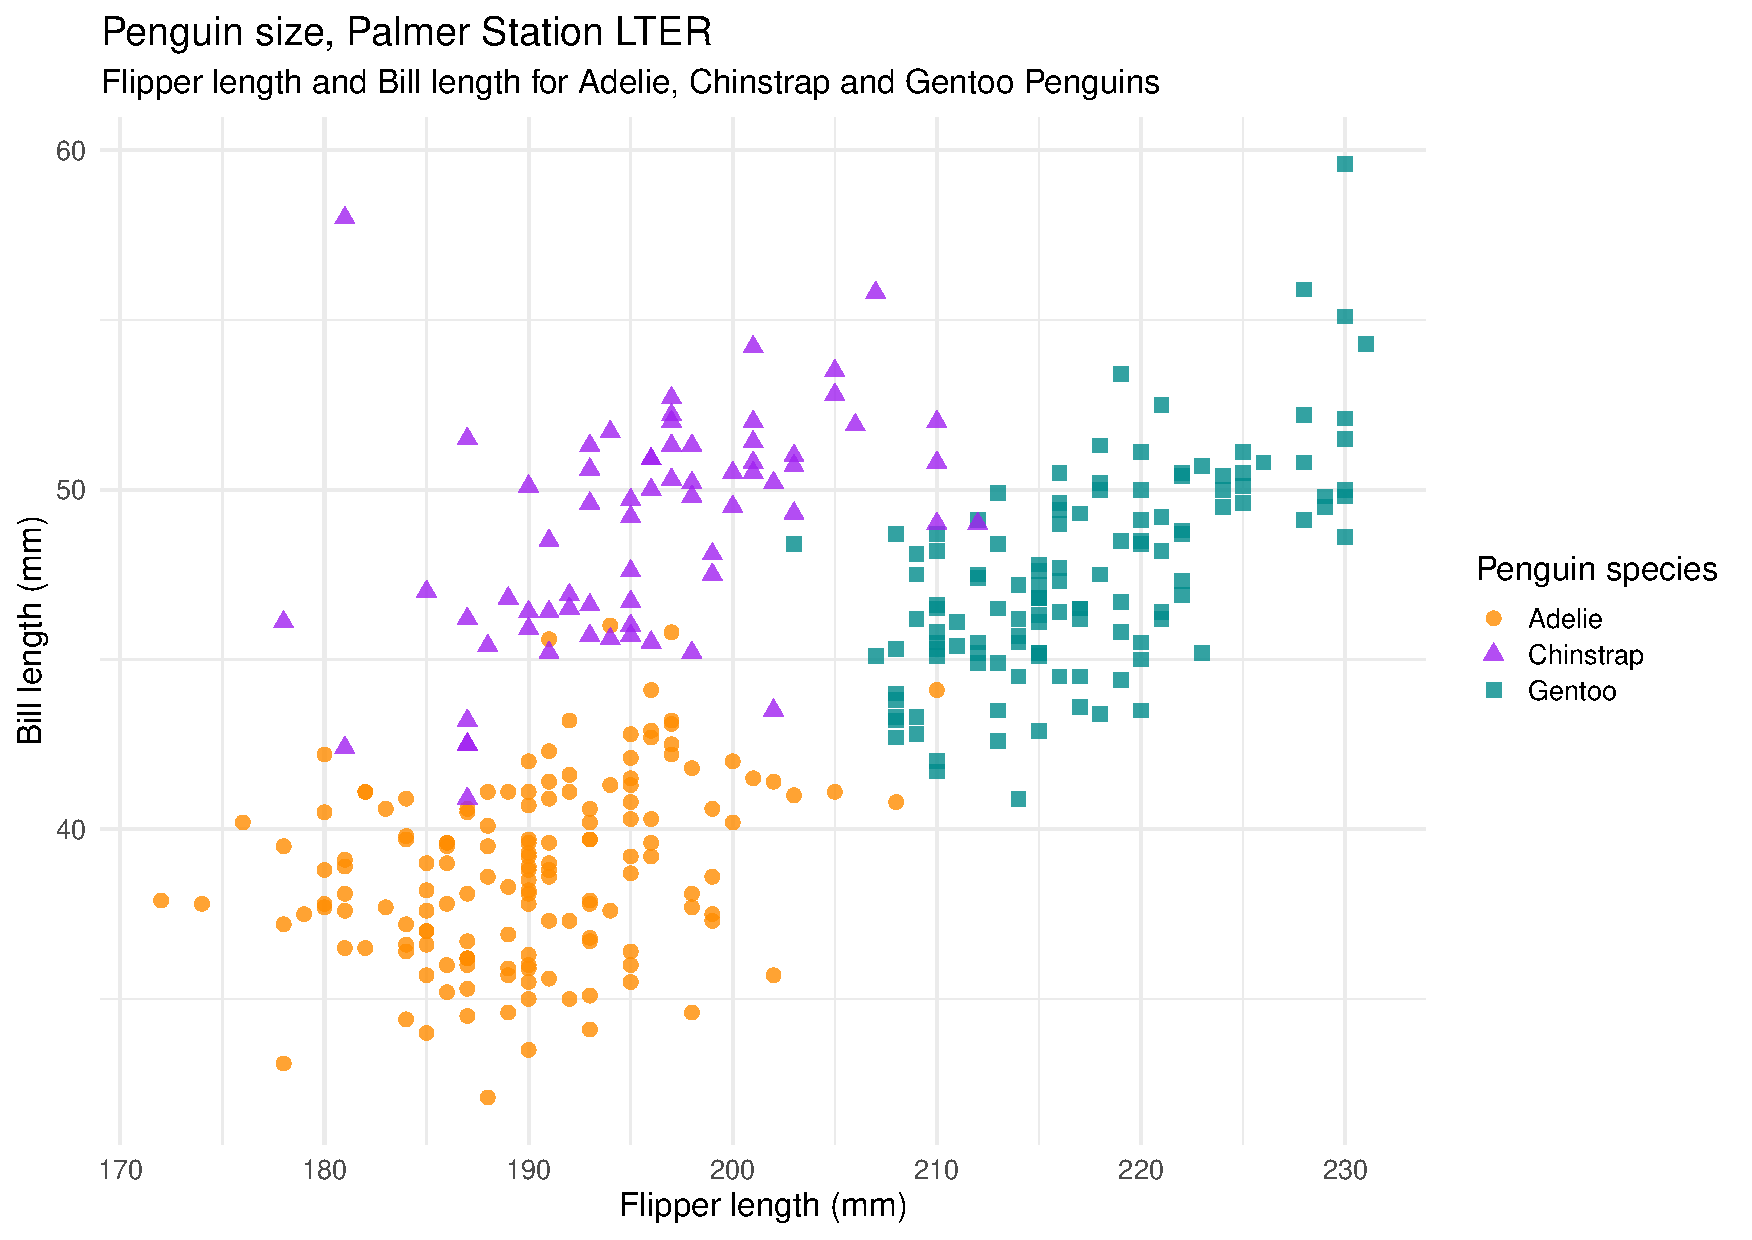
\includegraphics[width=\textwidth]{presentation/plotpen.pdf}
        \caption{Plot of Penguins}
        \label{fig:plotpen}
    \end{subfigure}

    \begin{subfigure}[b]{0.4\textwidth}
        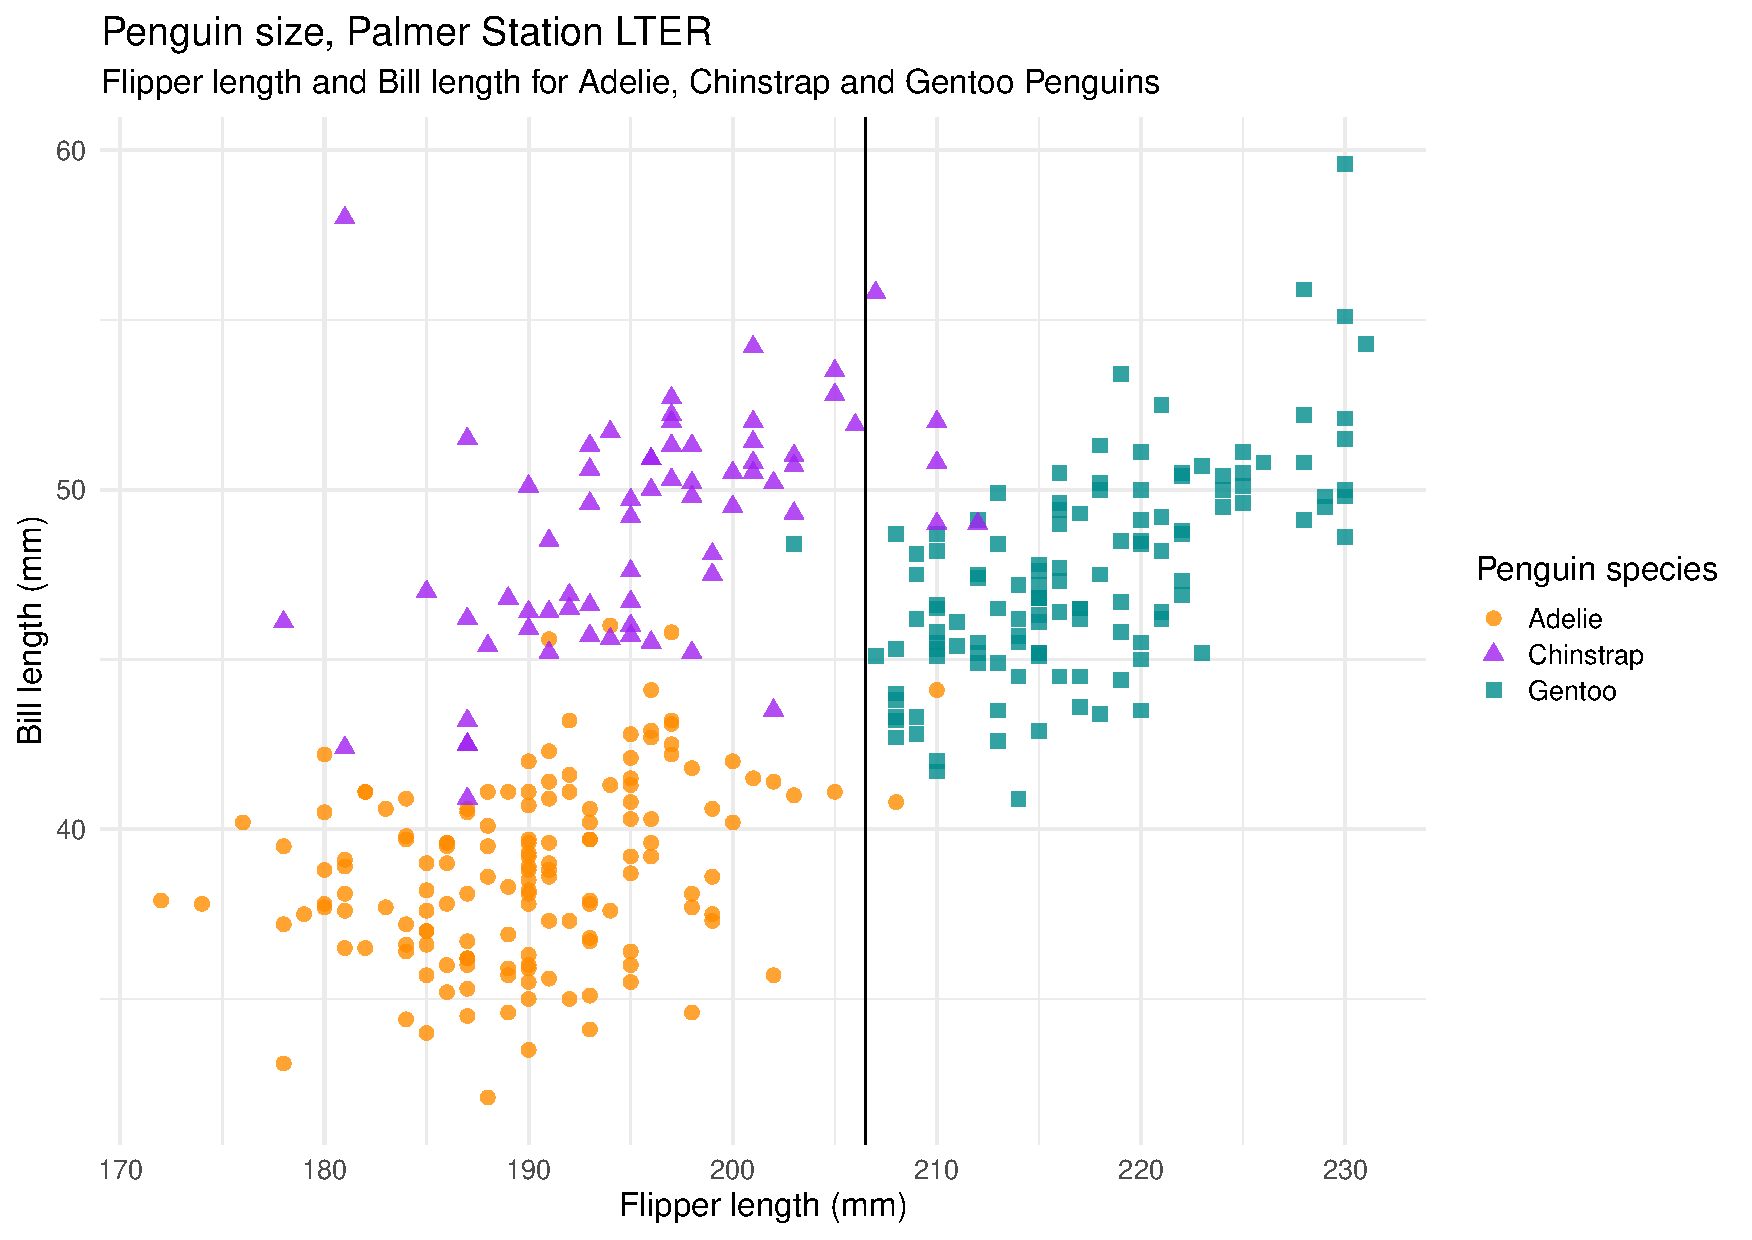
\includegraphics[width=\textwidth]{presentation/plotpen1.pdf}
        \caption{x = 206.5}
        \label{fig:plotsplit1}
    \end{subfigure}
    \begin{subfigure}[b]{0.4\textwidth}
        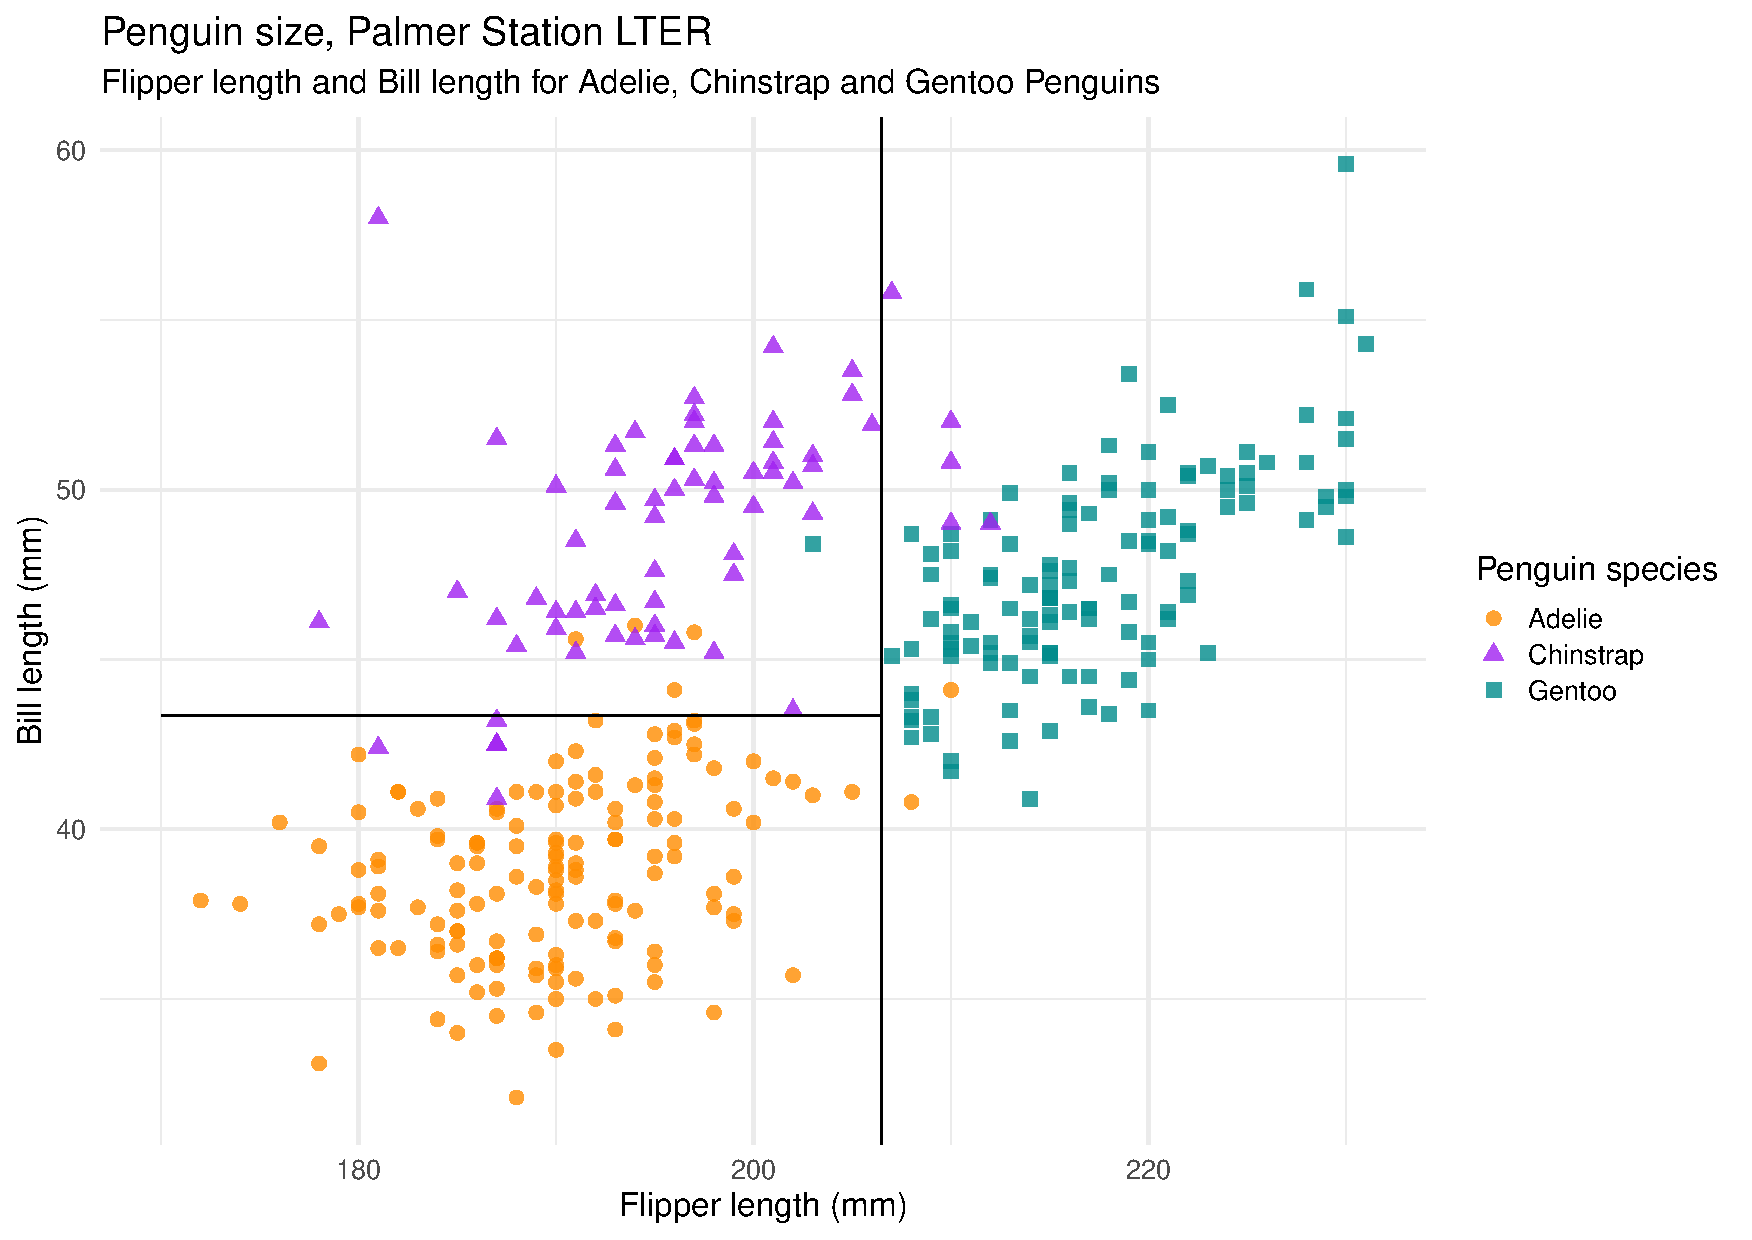
\includegraphics[width=\textwidth]{presentation/plotpen2.pdf}
        \caption{On left split, y = 43.35}
        \label{fig:plotsplit2}
    \end{subfigure}
    \caption{An Example of CART using Penguins}\label{fig:Penguins}
\end{figure}


\section{Programming Language}
For this project, we will be mainly using R as the main programming language although occasionally we might encounter situations where other languages such as Python or Julia turn out to be more convenient/easier to use. This is entirely dependant on the person and their personal preferences.\\
In many cases, it is possible to use at least 2 different languages for the entire process due to the convenience that each bring for the step needed. Often this occurs when we use one
language for data cleansing and another for the analysis and sometimes a third for producing the plots. There is no set order to this and you may use any language you wish.
Note that you will have to install external packages which do not come pre-installed with the programme. In such cases, you will have to install the package before running the code.

\subsubsection{R}
In {\color{blue} \texttt{R}} \cite{R}, this will be through the Comprehensive R Archive Network (CRAN) which maintains all packages that will be required for this project. When you need to install a new package, run the following line \textit{once}, the first time:
\begin{minted}{R}
install.packages("package")
\end{minted}
To work with data sets we will be using the {\color{blue} \texttt{dplyr}} \cite{dplyr} package which is part of the Tidyverse Library and is used for data manipulation. We will also be using {\color{blue} \texttt{ggplot2}} \cite{ggplot} to produce plots as this package produces better plots than the regular plot function.

\section{Dataset}
The Lahman Dataset is the largest publicly available dataset on baseball. It is part of the Baseball Archive set up by Sean Lahman in 1995 and the Baseball Dataset itself first appeared in 1996 and has been updated annually and maintained by a team of support staff \cite{Lahman} \footnote{Sean Lahman, Chris Dalzell, Michael Friendly, Dennis Murphy, Martin Monkman, Vanessa Foot, Justeena Zaki-Azat}. There is a .csv version, an SQL version, and R version (which is available through the CRAN). We will be using the R version to simplify the necessary data preparation.

\subsubsection{Description}
The following is the description of the data which has been sourced from the Lahman reference manual.\cite{Lahman}\\
\say{\textit{This database contains pitching, hitting, and fielding statistics for Major League Baseball from 1871 through 2019. It includes data from the two current leagues (American and National), the four other ``major" leagues (American Association, Union Association, Players League, and Federal League), and the National Association of 1871-1875.
This database was created by Sean Lahman, who pioneered the effort to make baseball statistics freely available to the general public. What started as a one man effort in 1994 has grown tremendously, and now a team of researchers have collected their efforts to make this the largest and most accurate source for baseball statistics available anywhere.}}\footnote{CRAN reference manual: https://cran.r-project.org/web/packages/Lahman/Lahman.pdf}



\section{Train and Test data}
When building models, we have to give prior information to teach the model what it needs to know.
What happens is that we will split the data into a learning class and a prediction class. 
In the learning class, we will further split the data into \textit{training} and \textit{testing} data, normally with around 70\% of the data being for \textit{training}. 
This is usually done automatically, and randomly, by the algorithm for each model.
For each algorithm, the training data will be used to teach the model how each factor affects the output and the testing data will be used to verify the results to make sure that the model is within the bounds of error.
\medskip\\
In this project, we have two data sets to work with for classification and regression respectively, where I showed the code for extracting the data in the Appendix.
Doing this, I am able to avoid having to further split the data into smaller training and testing sets which is better for testing the accuracy of the models.

\subsection{Why Train and Test Datasets}
\subsubsection{Training Data}
Clearly, the Train Data is used as a set of examples to teach the model where to fit the boundaries for the model. 
Without restrictions, this would allow us to draw perfect boundaries around the data set. However, new data would be poorly fit so the model would often draw more generalized boundaries which roughly fit the training data.
\subsubsection{Validation}
Within the training data, some training inputs are held back and used as \textit{validation} data.
This data is used to test the data as it learns and adjusts the \textit{tuning parameters} as well as give an error estimate of the final model once learning is completed.
\medskip\\
To avoid bias from subset selection, we use \textbf{cross-validation} as a technique to reduce bias from selection.
In this case, 10-fold Cross-Validation is the preferred method used in Statistical Machine Learning as it provides a good number of validation trials while not being as computationally taxing as higher folds would result in.
With 10-fold CV, we split the data into 10 ``folds" - $P_i$ - of equal size and then train the model 10 times, leaving out fold $P_i$ in each run and using said fold to test the accuracy of the model at that stage before tuning for the next model.
For each run, each fold has an accuracy $F_i$ and the overall accuracy of the training model is given as follows:
\[ 
\texttt{CV} = \frac{\sum_{i=1}^{10} F_i}{10} 
\]
\subsubsection{Testing Data}
On the other hand, testing data is used as a test once the model has been fitted.
This testing data is a completely new sample and is used to check the performance of the model given new data which the model has not seen previously. 
The measure of model performance is how well the model does when given the testing data. 

\section{Checking for Accuracy}
My aim for this project is to show how we have progressed from the basic CART algorithm and are now able to more accurately predict outcomes using the same information.
Thus it is crucial that we use the same datasets for each model that we build.
In order to test for performance, we have some methods for this:
\subsection{Checking Accuracy for Regression}
For Regression, it is trivial to use the errors in prediction as a variable to check accuracy.
In this case, we use the \textbf{Root-Mean-Square Error} (RMSE) which is defined as follows:
\subsubsection{Root-Mean-Square Error}
\begin{definition}[RMSE]
    The RMSE value is defined as the square root of the expected value of the square of the difference between $\hat{y}_i$ estimator and $y_i$ actual value 
\end{definition}
Thus, the RMSE is as follows:
\begin{equation}
    RMSE = \sqrt{\frac{\sum_{i=1}^{n} (\hat{y}_i - y_i)^2}{n}}
    \label{eq:RSME}
\end{equation}
Fortunately the \texttt{accuracy} command calculates and provides the RMSE value for us so this is easy to extract.

\subsection{Checking Accuracy for Classification}
For Classification, we create an error matrix referred to as the \textbf{Confusion Matrix}, which shows how ``confused" the model is when making predictions. 
This is a visual representation of the accuracy rate of the model which is calculated as such:
\begin{equation}
   \texttt{accuracy} = \frac{\texttt{correct predictions}}{\texttt{total predictions}}
   \label{eq:accuracy}
\end{equation}


\subsubsection{Confusion Matrix}
A Confusion Matrix classifies how well a model did into a table:
\begin{center}
\begin{tabular}{|c|c|c|c|}
    \cline{3-4}
    \multicolumn{2}{c}{} & \multicolumn{2}{|c|}{True Value}\\
    \cline{2-4}
    \multicolumn{1}{c|}{} & Total &  Actual Positive & Actual Negative \\ 
    \hline
    \multirow{2}{*}{Predicted Value} & Predicted Positive & \cellcolor{green} True Positive & \cellcolor{red} False Positive \\ 
    \cline{2-4}
    & Predicted Negative &  \cellcolor{red} False Negative & \cellcolor{green} True Negative\\
    \hline
\end{tabular}
\end{center}
We note that typically, a {\color{red} False Positive} is a \texttt{Type I Error}, and a {\color{red} False Negative} is a \texttt{Type II Error}.

\subsubsection{Receiver Operating Characteristic}
A better method to show how well the model performs is to use the \textbf{Receiver Operating Characteristic Curve} (ROC Curve). 
It is a graphical plot which uses probability predictions to show how accurate our model is.
We plot the True Positive Rate (TPR) on the y-axis against the False Positive Rate (FPR) on the x-axis.
A good model aims to maximise the \textbf{Area Under the ROC Curve} (AUC), which is the \underline{entire} area below the ROC Curve on the graph. 
The aim here is to get as close to \texttt{AUC = 1} as possible.
\bigskip\\
Conversely, a poor model would have \texttt{AUC < 0.5}. 
For reference, we plot the line $y = x$, the ``chance line", and if the curve is below this line, we consider this a bad model and a poor predictor which we would not be able to use.
\bigskip\\
For this we will be using {\color{blue} \texttt{ROCit}} \cite{rocit} which is the new ROC plotting function for R. 
A feature that {\color{blue} \texttt{ROCit}} provides is that it calculates the \textbf{Youden J Index} \cite{youden}:
\[ \texttt{J} = \frac{\texttt{True Positive}}{\texttt{Actual Positive}} + \frac{\texttt{True Negative}}{\texttt{Actual Negative}} - 1 \]
Where the optimal point is shown on the plot.
Each J Index calculates the likelihood that a Positive result is actually a True Positive. 
While this is not as useful for our data, it is very useful for medical data as it estimates the probability of an informed decision.



\section{Notation}
Before we proceed, it is necessary to state the notation that will be used in this paper.
\begin{itemize}
    \item $n$ the number of values at each point
    
    \item $M$ the number of groups we form after splitting/partitioning
    
    \item $\{x_{i},y_{i}\}_{i=1}^{n}$ the full dataset
    
    \item $x_{i}$ the input variables
    
    \item $y_{i}$ the dependent variable
    
    \item $\hat{y}_{i}$ the predicted value $y_{i}$

\end{itemize}
From here, we are able to proceed onwards with Decision Trees.


\chapter{AID, CHAID and The Original Decision Trees}
The idea of decision trees is to split up the data into segments (this is called \textit{segmenting}) and then keep breaking them down until we get suitable groups. This can then be summarized up into a tree which can be displayed to see the paths taken.

\section{Basics on Decision Trees}
Trees are basically graphs to show structure and flow.
A general idea is to think of a continuous variable $Y$ and some inputs $X_i ,  i = 0,...,n$. Lets say for simplicity, we have for two variables $X_1, X_2$ (thus creating a 2-D plane), we are able to create two separate regions from a partition, which we then model $Y$ on. This partition is on either $X_1$ or $X_2$. \\
Then, we are able to repeat the process for either one or both regions and model $Y$ on the new partitions and continue to do so until we get to a stopping point.
\\
The first question we ask is \underline{how do we know where to split each branch the tree?}

\section{AID}
\textbf{Automatic Interaction Detection (AID)} was first developed in 1963 by Morgan and Sonquist as a social science problem \cite{AID} as an optimization problem to sequentially partition data in an observation matrix into a binary regression tree \cite{ORAID}.
However, since then, it has proven so useful that it has become the basic building block for Decision Tree methods.

\subsection{AID algorithm}
The notation for this algorithm was based on source \cite{EarlyTree}:

\subsubsection{ANOVA}
Using Analysis of Variance (ANOVA), we can calculate the following:
\medskip\\
For a value $y_{im}$, $i \in [1,\dots,n]$, $m \in [1,\dots,M]$.
\begin{description}
    \item[Residual Sum Squares (RSS)] - The sum of the squares of residuals for each group (Also known as Within Sum Squares (WSS))
    \begin{equation}
        RSS = \sum_{m=1}^{M} \sum_{i=1}^{n} (y_{im} - \Bar{y}_{m})^{2}
        \label{eq:RSS}
    \end{equation}
    \item[Total Sum Squares (TSS)] - The sum of squares for all values
    \[
        TSS = \sum_{m=1}^{M} \sum_{i=1}^{n} (y_{im} - \Bar{y})^{2}
    \]
    \item[Between Sum Squares (BSS)] - where BSS = TSS $-$ RSS. Which is equivalent to the sum of squares for regression.
    \item[\textbf{$\eta^2$}] - A coefficient we aim to maximise. This is the ratio: $\frac{BSS}{TSS}$
\end{description}

\subsubsection{Steps for AID algorithm}
The AID algorithm is performed stepwise - it starts with a single cluster and calculates the splits one step at a time until a stopping point is reached. 
\begin{algorithm}
\begin{enumerate}
    \item At each step, for each predictor, either of the following occurs \cite{WilkinsonAID}:
    \begin{itemize}
        \item \textbf{Continuous Predictors} - For all $n$ cases, we have $n-1$ ways to split the cluster.
        Calculate the RSS value and select the optimal value.
    
        \item \textbf{Categorical Predictors} - All $2^{k} - 1$ possible splits between $k$ categories are checked.
        Calculate the RSS value and select the optimal value.
    \end{itemize}
    \item After calculating all RSS values we select the point with the smallest RSS value.

    \item We then consider the \textit{interaction} between predictors as we move down the levels as we no longer consider the same predictors for separate branches of the tree for the next stepwise calculation.
    
    \item Repeat the process until stopping point is reached.
\end{enumerate}
\caption{AID Algorithm}
\end{algorithm}

\subsection{Benefits of AID}
AID was a breakthrough in figuring out interactions between variables. It made possible, the idea of interaction between variables which helped solve many social science problems such as average earnings which previously have been difficult to solve if categorical variables have been included.
It is also one of the least taxing computationally but does show its age.
\medskip\\
Most importantly, AID was easy to interpret by non mathematicians and is highly visual, thus making them appealing in presentations.


\section{CHAID}
\textbf{CHAID} was developed by Kass in 1980 \cite{CHAID}.
It is essentially an extension of the AID algorithm suited for classification and stands for Chi-square Automatic Interaction Detection.\\
CHAID uses chi-squared statistical significance to test for significance of variables:
\begin{equation}
    \chi^{2} = \sum_{i = 1}^{n} \frac{\sqrt{(y_{i} - E(y_{i}))^2}}{E(y_{i})}
    \label{eq:chisq}
\end{equation}
Where $E(y_{i})$ is the expected value of $y$.\\
We select the splitting point to be the point with the highest value and continue until no significant $\chi^2$ value can be found.

\subsubsection{CHAID Algorithm}
Here we state Kass's CHAID algorithm \cite[pp. 121]{CHAID}.\\
For a given data table with a contingency table, we perform the following algorithm on the table:
\begin{algorithm}
\begin{enumerate}
    \item For each predictor, perform cross-tabulation of categories and then do the following:
    \begin{enumerate}
        \item Pair up categories of predictors which are the least significantly different. Merge both if they do not reach the critical value of the $\chi^{2}$ significance test above
        
        \item Repeat this step until all similar pairs have been merged
        
        \item For categories formed from \textbf{at least two} merges, find the most significant binary split and perform a $\chi^{2}$ test to see if this split is significant
        
        \item Repeat until splits are no longer significant
    \end{enumerate}
    
    \item Calculate the significance of each merged predictor and select the highest chi-squared value. If that value turns out to be larger than a criterion value, split the data into subcategories
    
    \item Repeat until all partitions have been analysed
\end{enumerate}
\caption{CHAID Algorithm}
\end{algorithm}

\textbf{Note:} Here, we check the criterion value against a contingency table.
An issue arises when we reduce the table size when merging groups as this means we can no longer use the same contingency table as before.
Kass noted this when formulating the algorithm and proposed using Bonferroni corrections on the splitting criterion which he found to have improved the results. 
We will not go into detail of that but the reader may consult \cite[pp. 122-126]{CHAID} if they would like to look into this.

\subsection{Benefits of CHAID}
CHAID brings all the benefits of AID but applies them in a classification setting. While it has been superseded by other models which are much more accurate, CHAID is still one of the fastest and easiest to explain mathematically and interpret.



\section{Downsides of AID/CHAID}
AID and CHAID, while useful, suffers from some issues:
\begin{enumerate}
    \item They are heuristically greedy - The algorithm works in a top-down approach.\\
    Unfortunately, this is a computational constraint and comes up quite often in future methods.
    
    \item Stopping point not defined - The nature of the algorithm means that there is no defined stopping point unless defined by the user when initializing the algorithm. This leads to unnecessarily large trees which require pruning.\\
    This will be solved in CART and will be discussed in the next chapter.
    
    \item Focus not on prediction - The creators of AID/CHAID were more interested in segmenting data than making predictions. Therefore the splits are more associative than a data scientist would prefer.\\
    Nevertheless, we should not ignore AID/CHAID based on this alone and it is still useful, however, not optimal.
\end{enumerate}

\chapter{Modern Decision Trees}
To address flaws in optimizing AID/CHAID, modern methods to form decision trees were invented in the 1980s and are still used today.\\
\textbf{CART} was first introduced by Leo Breiman an others in the 1984 book \textit{Classification and Regression Trees} (CART) \cite{BreimanDT}.
Since then, it has become one of the most cited methods for machine learning since it is easy to interpret while maintaining its accuracy.\\
An alternative method was developed in 1986 by Ross Quinlan \cite{Quinlan} called \textbf{ID3}, which grew to become \textbf{C4.0, C4.5, C5.0 etc}. The method is very similar to Breiman's and really only differs in terms of the metrics used.




\section{Classification}
To find the best split for Classification Trees, we try to find the split which gives the least errors. This can be defined as a metric to simplify calculations.
There are \textbf{two} major metrics, and many more minor ones, that are used in deciding where to split each branch.

\begin{enumerate}
    \item \textbf{\textit{Gini Impurity}}: Used by the CART method \cite{BreimanDT}, 
    
    \item \textbf{\textit{Information Gain}}: Used in methods such as C4.5, ID3 \cite{Quinlan}
\end{enumerate}
A metric is considered a good metric if it performs better than the standard misclassification error.
\subsubsection{Misclassification Error}
\begin{definition}[Misclassification Error]
A measure of node impurity is called Misclassification Error.
\begin{equation}
    I_G (p) = 1 - \max (p_i, 1 - p_i)
    \label{eq:misclassificationerror}
\end{equation}
\end{definition}
The Misclassification Error line is the boundary in deciding whether the metric performs better than random guessing.
In this case, the majority voting group of the region is marked as $p_i$ and everything else is considered as misclassification.
One would think that this method would be the best method but we find that using this criterion, one ends up with relatively useless splits compared to the methods we will be introducing below.
\medskip\\
The thing one has to think about is that we are trying to see whether we improve prediction if one were to split.
When splitting, one tries to find the Loss Function $L$ which improves the model the most. 
Here, we define $L_{misclass}$ for misclassification error as
\[
L_{misclass} = I_G (p) = 1 - \max p_i
\]
and one tries to find the split which minimises $L$ as much as possible before and after splitting.
This is defined as follows,
\[
\min L(Parent) - (L(Child_1) + L(Child_2))
\]
Now, one can see that if you have a group which weighs, lets say $\{900,100\}$ and split it, one can achieve multiple splits which give groups, of equal $L$, which classify the same but of different sizes, i.e. $\{900,100\} \rightarrow \{700,100\} + \{200,0\}$ and $\{900,100\} \rightarrow \{400,100\} + \{500,0\}$ both have the same $L = 100$.
Thus, one needs to find a better metric to split on.

\subsection{Calculating metrics}
Metrics are based on the idea of Entropy, which itself is part of \textbf{Information Theory}, defined by Claude E. Shannon in 1948 in his landmark paper \textit{A Mathematical Theory of Communication}. \footnote{http://cm.bell-labs.com/cm/ms/what/shannonday/shannon1948.pdf} \cite{Shannon}. 
The aim here is to calculate a value, which we can then use to see if splitting at that node would improve the accuracy of our decision tree.

\subsubsection{Entropy}
\begin{definition}[Entropy]\cite{Shannon}
The Entropy of a random variable is defined as the information uncertainty in the variable's possible outcomes.
\end{definition}
In fact, Shannon had formulated this into a theorem for entropy which we will now state:
\begin{theorem}[Entropy] [Based on source \cite[Section 6, p. 10]{Shannon}]\\
For a measure $H(p_1,\dots,p_n)$ where $p_1 + \dots + p_n = 1$ and $p_i$ the probabilities which hold the following conditions:
\begin{enumerate}
    \item $H$ is continuous in $p_i$
    
    \item If all $p_i$'s are equal, then $H$ is monotonic
    
    \item If a choice is broken down into two successive choices, then $H$ becomes the sum of each individual values.\\
    \textbf{For Example}: $H(\frac{1}{2}, \frac{2}{5}, \frac{1}{10}) = H(\frac{1}{2}, \frac{1}{2}) + \frac{1}{2}H(\frac{4}{5}, \frac{1}{5})$
\end{enumerate}
If the above is satisfied, we can define entropy as:
\begin{equation}
    H(T) = I_E (p_1, \dots , p_n) = -\sum_{i=1}^{n} p_i \log_b p_i
    \label{eq:entropy}
\end{equation}
\end{theorem}
We can to derive two forms of entropy from the above:
\begin{enumerate}
    \item Entropy of one attribute (Parent Entropy):
    \begin{equation}
        H(T) = -\sum_{i=1}^{n} p_i \log_2 p_i
        \label{eq:pentro}
    \end{equation}
    This is the full data
    
    \item Entropy of two attributes (Child Entropy):
    \begin{equation}
       H(T \mid a) = -\sum_{i=1}^{n} P(i \mid a) \log_2 P(i \mid a) 
       \label{eq:centro}
    \end{equation}
    We have that $P(i \mid a)$ the proportion of the group that was split into one child node from the parent node.
    This is the filtered data and the sum of each group of Child Entropy's is equal to the Parent Entropy.
\end{enumerate}
We then use the two entropy's to calculate information gain.

\subsubsection{Information Gain}
\begin{definition}[Information Gain]
Information Gain is a measure to see how much information can be added if we were to split the tree node compared to keeping the node as it is:
\begin{equation}
    I_G(T,a) = H(T) - H(T \mid a) = -\sum_{i=1}^{n} p_i \log p_i
    + \sum_{i=1}^{n} P(i \mid a) \log_2 P(i \mid a) 
    \label{eq:ig}
\end{equation}
With probabilities $p_i$, and $P(i \mid a)$ the proportion of the group that was split into one child node $a$ from the parent node.
\end{definition}
Simply, we can subtract \ref{eq:centro} from \ref{eq:pentro} to get the Information Gain Value.
\medskip\\
Information Gain is used to decide on which feature to split on. We want it so that each split provides the most ``information" and is therefore the value with this highest $IG(T,a)$. If $IG(T,a) = 0$, then we have found a leaf node and stop, else repeat the process until we arrive at a leaf node. This metric is used in ID3 and C4.5 \cite{Quinlan}.

\subsubsection{Gini Impurity}
CART uses a method called \textbf{Gini Impurity} which measures how often we would incorrectly sort a random element from the set. 
While not directly formulated from Entropy above, it is similar enough that one should know both.
\begin{definition}[Gini Impurity]
The Gini Impurity (Also called Gini Index) can be defined as the following:
\begin{equation}
    I_G (p) = I_G (p_1, \dots, p_n) = \sum_{i=1}^{n} p_i(1-p_i) 
    \label{eq:gini}
\end{equation}
With $i=1,\dots,n$ classes and probabilites $p_i$ where $\sum_{i=1}^{n} p(i) = 1$
\end{definition} \cite{BreimanDT}
Our aim is to try to make \ref{eq:gini} = 0. 


\subsubsection{Whats the difference?}
While the two methods require different calculations, a paper by Murthy comparing these two methods among others \cite{murthy1995} found that there is no significant difference between Information Gain and Gini Impurity in the results to determine which is more optimal. 
However, when implemented into algorithms, CART, which uses Gini Impurity, while more efficient, can only partition the data into two groups whereas ID3 and C4.5 are able to split into multiple partitions at each point.
On the other hand, CART, by the nature of Gini Impurity, provides an efficient stopping algorithm which does not depend on restrictions put on by the user. This makes it the preferred method compared to Quinlan's method.
\begin{figure}
    \centering
    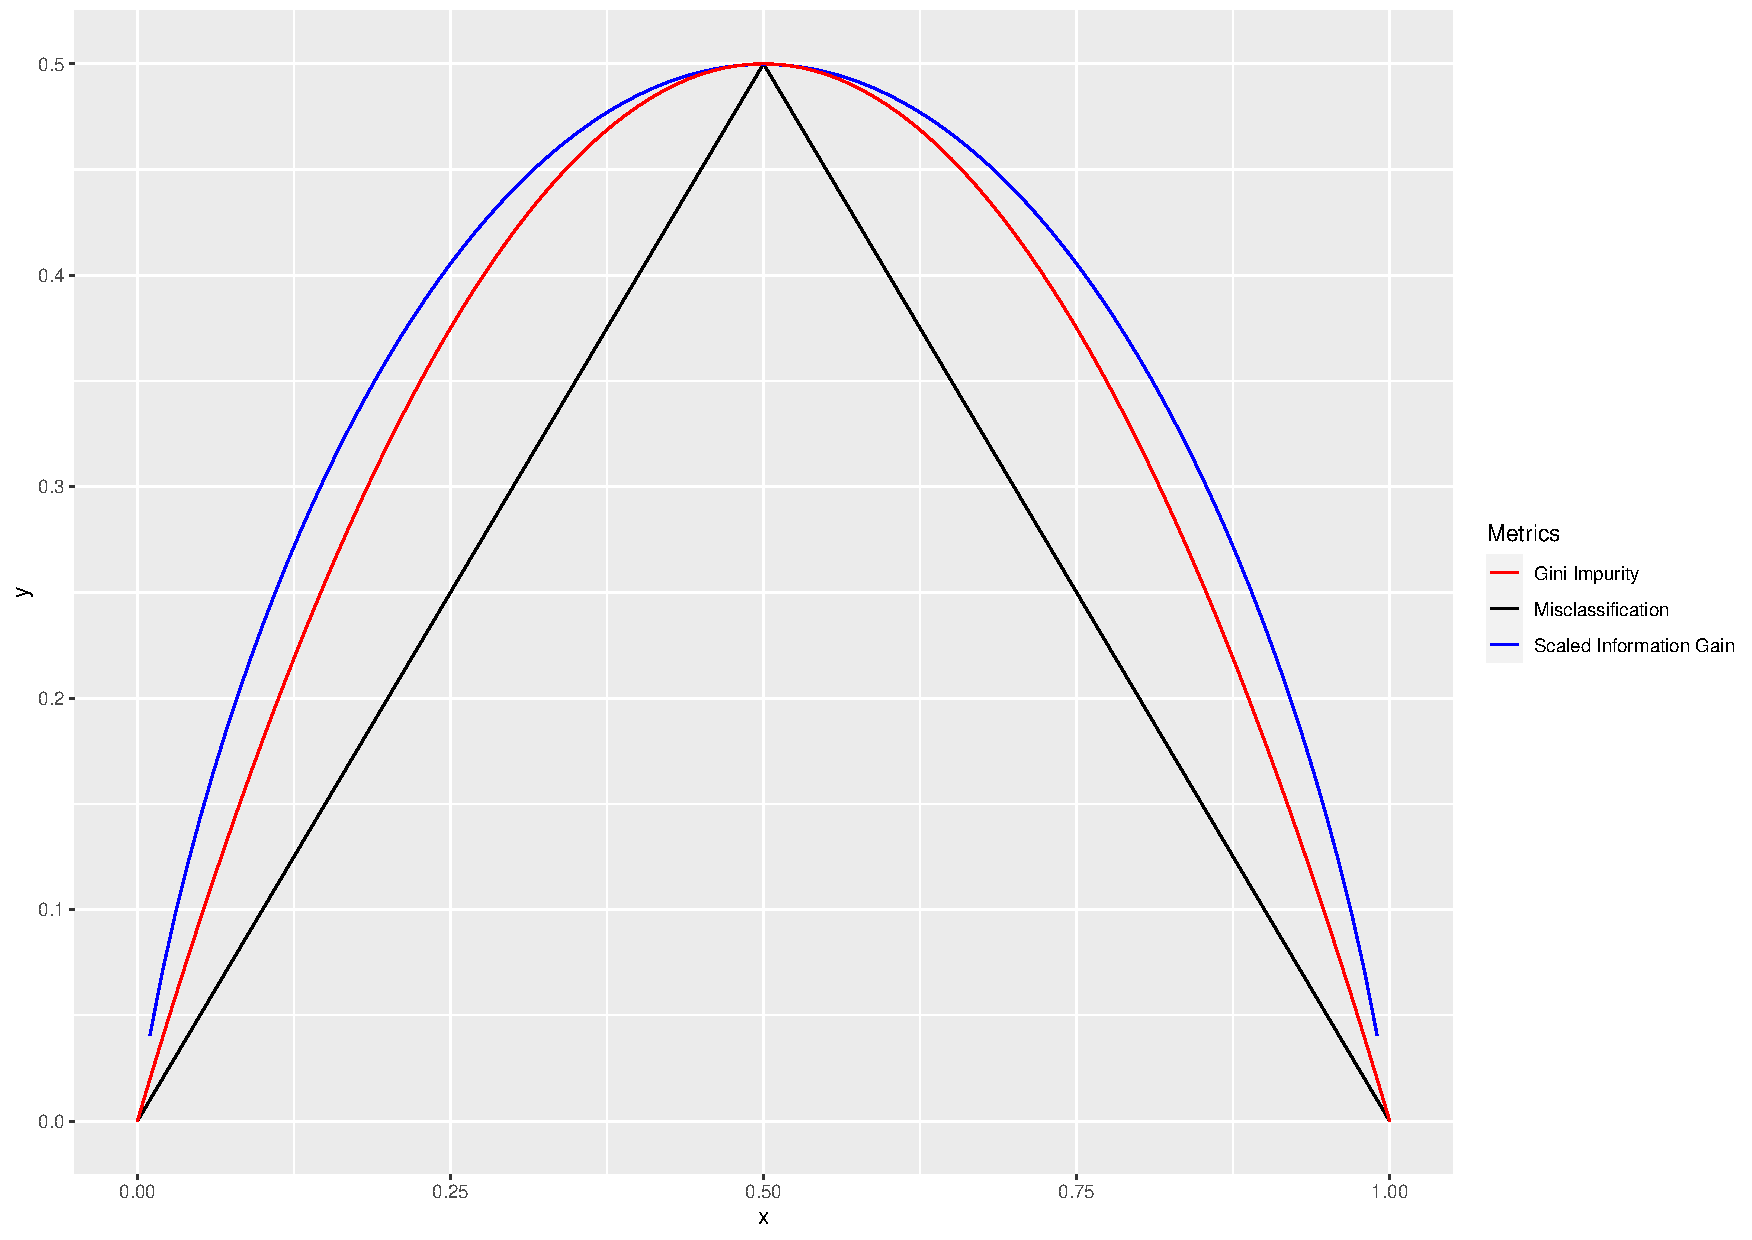
\includegraphics[width=8cm]{reportcharts/Metriccomp.pdf}
    \caption{Comparison of Metrics, Gini vs Information vs Misclassification}
    \label{fig:metrics}
\end{figure}
\medskip\\
Thus deciding on which to use depends on the end user and their preferences from the results of the algorithm. Here we will proceed with CART as it leads on nicely to Bagging and Random Forests.
\medskip\\
Before we proceed onto the algorithm, we note a final metric which is useful to know but not essential towards forming Decision Trees.

\subsubsection{Twoing Criterion}
This final criterion was introduced by Breiman in CART \cite{BreimanDT} along with Gini Impurity.
\begin{definition}[Twoing Criterion]
    Twoing is the grouping of all classes into two superclasses using the following:\\
    Given we send a proportion $P_L$ of the whole learning class to the left, and $P_R = 1 - P_L$ to the right, we find the best twoing split $s$ at node $t$ to be as follows:
    \begin{equation}
        I_G (p) = \frac{P_L P_R}{4} \left[ \sum_{j=1}^{J} \left| p_{j,L} - p_{j,R} \right| \right]^2
        \label{eq:twoing}
    \end{equation}
    Where $p_{j,L}$ and $p_{j,R}$ the probabilities that $p_j$ goes left or right respectively.
\end{definition}
Twoing balances purity and the creation of equal size nodes and is thus the best method since this allows us to consider the problem as a two class problem and lets us build a more balanced - and much better - tree.\\
However, this method is much slower than calculating Gini Impurity and is thus not often used and we are unable to perform this in {\color{blue} \texttt{R}}, only in the original {\color{blue} \texttt{Salford Systems'}} which CART was originally written for.



\subsection{CART Classification Algorithm}
The CART algorithm for classification is very similar to those we have already seen before. \\
For each variable $x_i$, $i \in [i, \dots, n]$ leading to a response $y_i$ where $y$ is a classification, we complete the following:
\begin{algorithm}
\begin{enumerate}
    \item For each variable at every point, split the data into two regions $R_1, R_2$ where:
    \begin{enumerate}
        \item $R_1 = x_i \leq s$
        \item $R_2 = x_i > s$
    \end{enumerate}
    
    \item Calculate the Gini Impurity for said split and test it against all other splits
    
    \item Select the value with the highest Impurity as the choice of split
    
    \item Repeat until stopping criterion is met
\end{enumerate}
\caption{CART for Classification}
\end{algorithm}





\section{Regression Trees}
Unlike classification, regression does not have natural groupings to simply work out calculations for where to split. 
Therefore an alternative method for partitioning needs to be found.
The method is to minimize the Residual Sum of Squares (RSS), similar to AID \ref{eq:RSS} but with some minor differences. \medskip\\
Here, we have that \cite[Section 3, p. 44-46]{ESL}:
\begin{equation}
  RSS = \sum_{i}^{n}(y_i -\hat{y_i})^2  
\end{equation}
From here, we now need to apply this idea to regions $m$.

\subsection{CART Regression Calculations}
\emph{Based off ESL \cite[Section 9, p. 307]{ESL}}\\
Suppose we have a space $R$ and we have $M$ partitions, we first partition the space into $M$ regions $R_1, \dots, R_M$.
Our aim is to predict which region the values $x$ fall into and take the average value of the region to make a predictor.\\
To construct the regions, we try to find regions which minimize RSS, where we have $\hat{y}_{R_m}$ as the mean response for each region:
\begin{equation}
    RSS = \sum_{m=1}^{M} \sum_{i \in R_m} (y_i - \hat{y}_{R_m})^2
\end{equation}
To construct this we use the following methods:
\subsubsection{Splitting points using RSS}
We have for each variable $x_i$, $i \in [1, \dots, n]$, leading to a predicted value $y_i$ 
\begin{algorithm}
\begin{enumerate}
    \item For each variable at every point, split the data into two regions $R_1, R_2$ where:
    \begin{enumerate}
        \item $R_1 = x_i \leq s$
        \item $R_2 = x_i > s$
    \end{enumerate}
    
    \item Calculate the following for each split:
    \begin{equation}
     \sum_{x_i \in R_1} (y_i - \hat{y}_{R_1})^2  +  \sum_{x_i \in R_2} (y_i - \hat{y}_{R_2})^2
    \end{equation}
    
    \item Select the minimal value in (2) for each variable and compare with all variables selecting the minimal value as the splitting variable.
    
    \item Repeat until stopping criterion is met
\end{enumerate}
\caption{CART Regression Algorithm}
\end{algorithm}


We model the response variable to the data with $N$ observations and $n$ inputs, which each have a response, as a constant $c_m$ in each region:
\begin{equation}
    f(x) = \sum_{m=1}^{M} c_m I (x \in R_m)
\end{equation}
Where we can obtain a optimum $\hat{c}_m$ which we find to be the average of $y_i$ for each region $R$.
\begin{equation}
    \hat{c}_m = av(y_i | x_i \in R_m)
\end{equation}

\subsection{Comparisons with AID}
We notice that both Regression CART and AID calculate the RSS values to figure out the residuals if we were to split at a point.
In fact, the algorithm is pretty much the same, although some minor differences can be found. 
The difference is really found in calculating the predicted value of the new child nodes, however, more often than not, this tends to be the same value in both cases.


\section{Pruning}
Often we get trees which are way too big and unnecessarily complicated when simpler trees often do the trick. 
This leads to overfitted trees which provide high bias and low variance and is therefore unsuitable for regular use.\\
Ideally, we would grow a small tree with a minimum split value at certain point.
However, the heuristically greedy nature of the algorithm would hide a very good split behind a seemingly weak split. 
To get around this, the alternative is to grow a very large tree $T_0$ and \textit{prune} them back to obtain a subtree $T$ instead where $T \subset T_0$.
We call this method \textit{Cost-Complexity Pruning} \cite{BreimanDT}.

\subsection{Cost-Complexity Parameter}
A quick explanation on the Cost-Complexity Parameter is useful to have before we proceed onto pruning.
The \textbf{Complexity Parameter} (cp) is another method used to control how big the tree can grow. 
The cp parameter is there so that if adding another split to this node leads to an increase in cp, the tree does not grow that node.
Knowing this, we can now work out the Cost-Complexity Pruning.

\subsection{Cost-Complexity Pruning}
The idea of pruning is to minimise the cost-complexity criterion:
\begin{equation}
    C_{\alpha} (T) = R(T) + \alpha \left|T\right|
    \label{eq:prune}
\end{equation}
Where $R(T)$ is the learning error, $\left|T\right|$ the number of terminal nodes in tree $T$, and $\alpha$ the regularization parameter.\\
$R(T)$ differs depending on the type of tree we are pruning:
\begin{itemize}
    \item For Classification: 
    \[ R(T) = \sum_{i = 1}^{T} (1 - \max (p_i, 1 - p_i)) \times \frac{n(t)}{n} \]
    Where $n(t)$ is the number of $x_i$'s in each $t$ leaf node and $n$ the total number of $x_i$'s
    
    \item For Regression:
    \[ R(T) = \sum_{m=1}^{T} \sum_{i \in R_m} (y_i - \hat{y}_{R_m})^2 \]
\end{itemize}

\subsubsection{Pruning a Subtree}
To prune a subtree, lets look at an individual subtree $T_t$. 
The aim here is to minimise the following:
\[ 
\begin{split}
    C_\alpha(T-T_t) - C_\alpha(T) &= R(T-T_t)+ \alpha|T-T_t| - (R(T)+ \alpha|T|)\\
    &=R(T-T_t)-R(T)+\alpha(|T-T_t|-|T|)\\
    &=R(T)-R(T_t)+R(t)-R(T) + \alpha(|T|-|T_t|+1-|T|)\\
    &=R(t)-R(T_t) + \alpha(1-|T_t|)\\
\end{split} \]
Which results in the following value of $\alpha$
\[ \alpha = \frac{R(t)-R(T_t)}{|T_t| - 1} \]
\textbf{Note:} If $\alpha = 0$, then we return the whole tree unpruned so we aim to look at cases when $\alpha \neq 0$.

\subsubsection{Algorithm}
The Algorithm for pruning is as follows \footnote{mlwiki.org/index.php/Cost-Complexity\_Pruning}:
\begin{algorithm}
\begin{enumerate}
    \item Initialization - Let $T^1$ be the tree obtained with $\alpha^1 = 0$ by minimizing $R(T)$
    
    \item Step 1.1 - Select $t \in T^1$ which minimizes
    \[ g_1 (t) = \frac{R(t)-R(T_t^1)}{|T_t^1| - 1} \]
    
    \item Step 1.2 - Let $t_1$ be this node and let $\alpha^2 = g_1 (t_1)$ which results in $T^2 = T^1 - T_{t_1}^1$
    
    \item Repeat - Repeat the process $i$ times until at cost $k$
\end{enumerate}
\caption{Pruning Algorithm}
\end{algorithm}

This results in the following outputs:
\begin{itemize}
    \item a sequence of trees up to the root node: $T^1 \supseteq T^2 \supseteq \dots \supseteq T^k \supseteq \dots \supseteq T^{root}$
    
    \item a sequence of parameters $\alpha^1 \leq \alpha^2 \leq \dots \leq \alpha^k \leq \dots$
\end{itemize}
We now choose $\alpha^k$ which is our optimal value and then obtain the corresponding tree $T^k$ as our result.
\bigskip\\
\textbf{Note:} If one were to grow a tree and compare that tree to one which had been pruned from that tree, we would fine that \underline{this} pruned tree would perform worse than the normal tree.
One should aim to use pruning as a method to simplify trees while minimizing the accuracy lost.





\section{Implementation of CART}
There have been multiple implementations of CART over the years. The most famous of these is {\color{blue} \texttt{rpart}} \cite{rpart}, which is what we have used for this project. 
Here we will use the two sets of data which were put together in the introduction and I will provide a summary of it below.

\subsection{Using {\color{blue} \texttt{rpart}} for CART and ID3}
One of the great features of {\color{blue} \texttt{rpart}} is that it allows you to create many different styles of Decision Trees based on what restrictions you give the model.
\medskip\\
By default, {\color{blue} \texttt{rpart}} uses Gini Impurity as the main metric for splitting. 
However, one can use ID3 in this scenario by selecting the parameter \texttt{parms=list(split="information")} which makes {\color{blue} \texttt{rpart}} apply Information Gain as the splitting metric.
Here, we end up producing different trees, however, one can see that the difference is relatively negligible as we see from an extract from {\color{blue} \texttt{R}} from our example we will refer to later.
\begin{minted}[frame = single]{R}
          nlwinpred
infonlpred    0    1
         0 1358   22
         1   51   58

[1] "Accuracy for test 0.950973807924782"
\end{minted}

\subsection{Implementing CART in R}
Using {\color{blue} \texttt{rpart}} without applying any control metrics gives us the following Decision Tree:
\begin{minted}[frame = single]{R}
lgwinfit <- rpart(LgWin ~ ., data = alplayoff1)
#Using all available variables as possible predictors

lgwinfit
n= 1265 

node), split, n, loss, yval, (yprob)
      * denotes terminal node

 1) root 1265 118 0 (0.90671937 0.09328063)  
   2) W< 94.5 1108  33 0 (0.97021661 0.02978339)  
     4) L>=65.5 990  12 0 (0.98787879 0.01212121) *
     5) L< 65.5 118  21 0 (0.82203390 0.17796610)  
      10) ERA>=3.295 71   5 0 (0.92957746 0.07042254) *
      11) ERA< 3.295 47  16 0 (0.65957447 0.34042553)  
        22) E>=186.5 34   7 0 (0.79411765 0.20588235) *
        23) E< 186.5 13   4 1 (0.30769231 0.69230769) *
   3) W>=94.5 157  72 1 (0.45859873 0.54140127)  
     6) L>=57.5 106  38 0 (0.64150943 0.35849057)  
      12) X3B< 34.5 62  15 0 (0.75806452 0.24193548) *
      13) X3B>=34.5 44  21 1 (0.47727273 0.52272727)  
        26) SV< 26.5 10   1 0 (0.90000000 0.10000000) *
        27) SV>=26.5 34  12 1 (0.35294118 0.64705882)  
          54) BBA< 488.5 16   7 0 (0.56250000 0.43750000) *
          55) BBA>=488.5 18   3 1 (0.16666667 0.83333333) *
     7) L< 57.5 51   4 1 (0.07843137 0.92156863) *
\end{minted}
Which results in the following Decision Tree \ref{fig:classtreeex}:
\begin{figure}
    \centering
    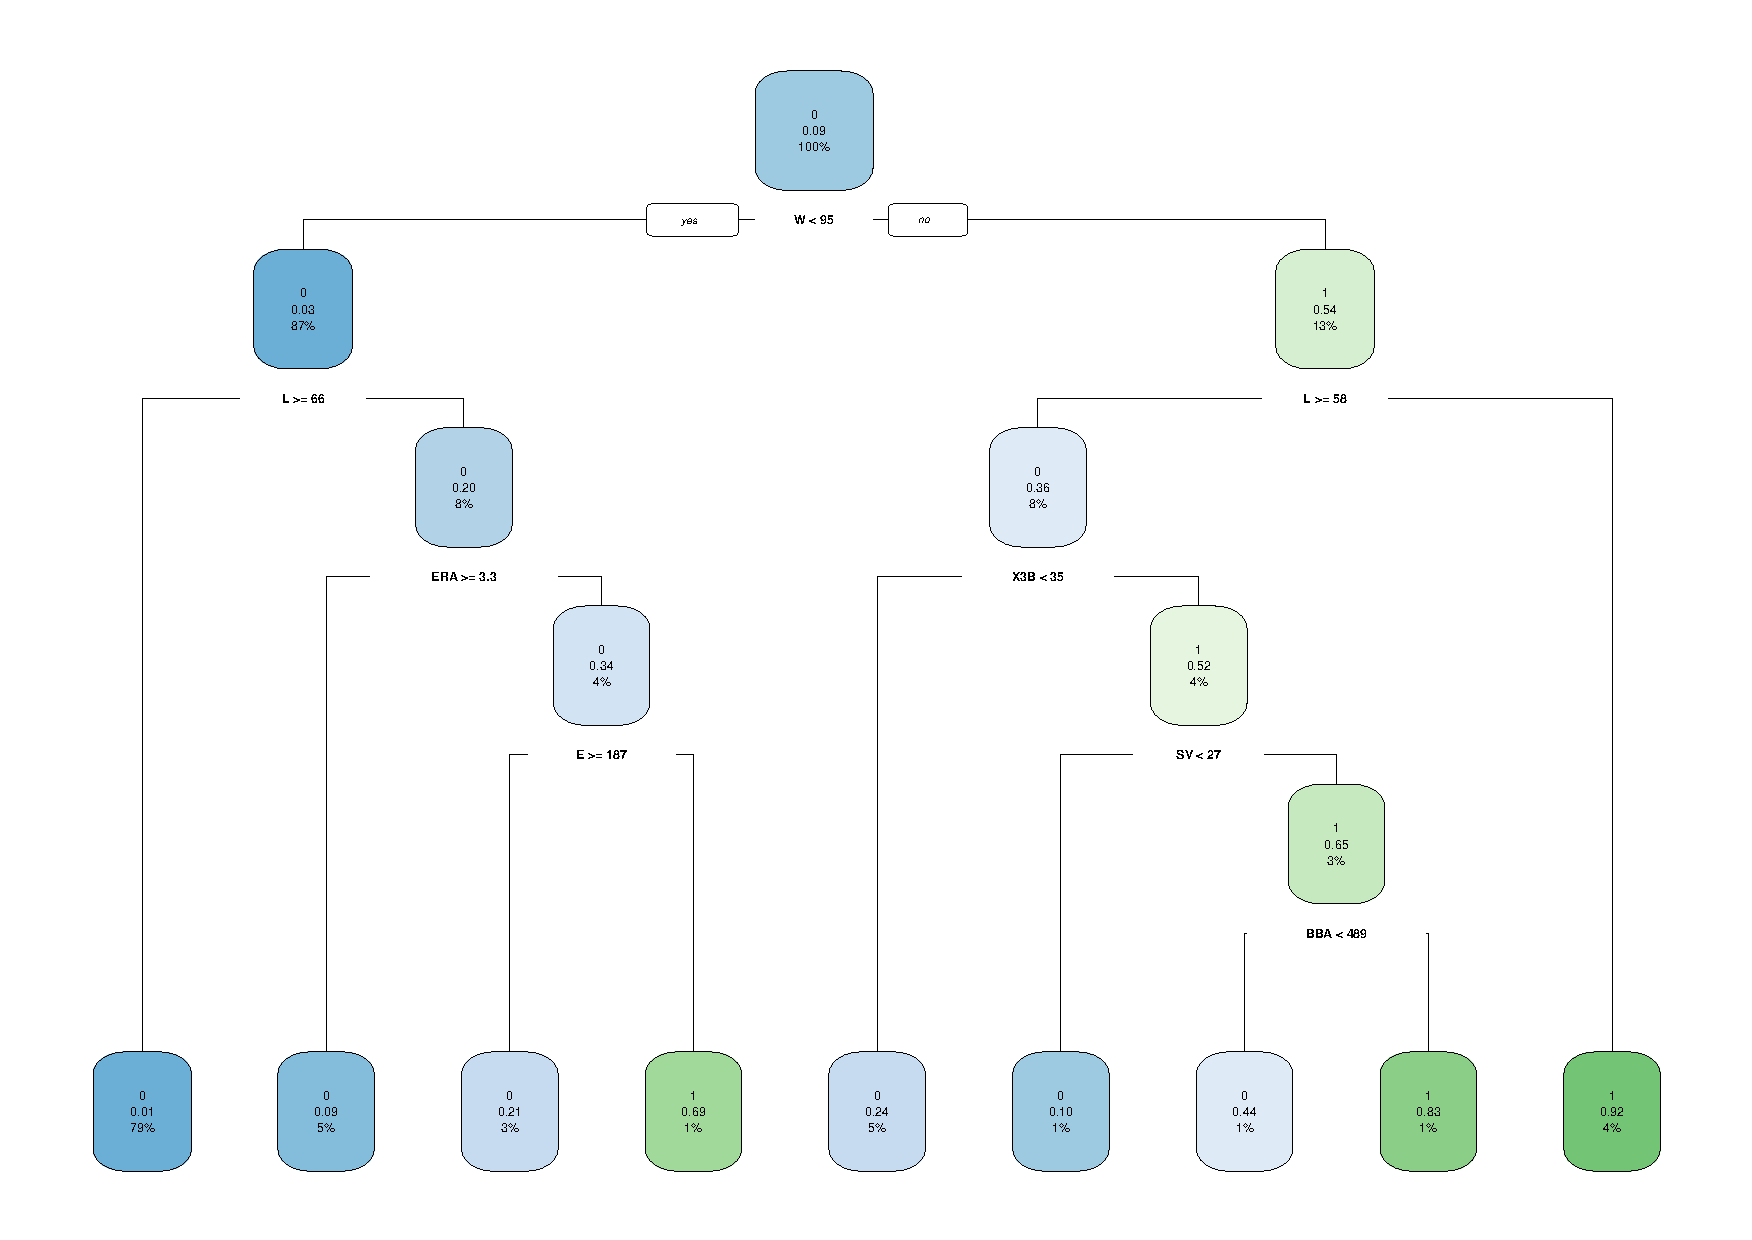
\includegraphics[width=10cm]{finalplots/classtree.pdf}
    \caption{Example of a Decision Tree using CART}
    \label{fig:classtreeex}
\end{figure}


\section{Tree Depth}
The default parameter when growing a tree has a minimum number of variables before splitting at \texttt{minsplit = 20} and a maximum tree depth \texttt{maxdepth = 10} among other variables.
Applying different control parameters lead to different size decision trees and one may prefer to increase the maximum tree depth if the dataset is large enough that our stopping criterion is hiding major splits.
\medskip\\
The change in tree due to changes in tree depth leads to changes in accuracy. 
One finds that a larger tree depth leads to much more accurate trees, but going too far can lead to over-fitting which counter-intuitively leads to a reduction in accuracy with very large trees, which then have to be pruned to achieve interpretability.
Thus, when building trees, one should carefully select the size of the tree which is the best predicting model while maintaining interpretability.


\section{Flaws of CART}
CART, while a major improvement over other methods, does have its flaws like all methods do:
\begin{enumerate}
    \item Heuristically greedy - Similar to AID/CHAID, the top-down approach leads to greedy splits where good splits are hidden behind a split which looks strong, but is actually a terrible split as it masks other more appropriate splits.
    
    \item Binary nature of Split - The Gini Impurity metric only works for binary splits (Each parent node can only split in two and not more than that).\\
    Fortunately, other methods such as ID3 and C4.5 using alternative metrics are able to perform better splits in that regard.
    
    \item Complexity of Trees - This is both taxing in terms of computer memory and in terms of size. \\
    Unfortunately, pruning is the only method to achieve a desirable tree without losing any major splits if we were to grow a very small tree instead.
\end{enumerate}

\chapter{Bagging and Boosting - Ensemble Methods}
While being easy to interpret as well as flexible for many problems, there have been many attempts to improve upon decision trees.
This has led to the development of two different tree based methods which when combined, create a much better predictor:
\begin{enumerate}
    \item \textbf{Bagging/Random Forest} - Based on the idea of bootstrapping techniques to create many trees from randomly selected samples \cite{bootstrap}, with replacement, from the full learning set
    
    \item \textbf{Boosting} - Using weak learning trees to learn from incorrect predictions when forming successive trees
\end{enumerate}
Both use the idea of ``black-box" learning of trees but differ in the way they use decision trees when learning. 
Simplistically, Bagging/Random Forests grow trees co-currently in parallel with each other whereas Boosting grows trees successively, learning from previous mistakes. 

\section{Bagging vs Boosting}
Bagging/Random Forests are used to reduce the variance of Decision Trees by aggregating lots of trees together to create a stronger predictor.
Since each sample is independent of one another, when combined, we have found a method to reduce the overall variance of the model. 
However, we have not introduced any bias to the model by bootstrapping the samples.
\medskip\\
Conversely, Boosting is used to reduce bias in Decision Trees since they aim to ``learn" from the errors of previously grown weak learners.
Boosting also combines results as it grows each tree and thus each new prediction is somewhat related to previous predictions from older weak learners.
\bigskip\\
We note that clearly, both methods lose the interpretability of CART as it is not feasible to show how all trees are grown.
However, this is often offset by the shear superior accuracy that these models produce compared to regular Decision Trees.
Therefore, we find these methods are often used when the prescriptive aspect of the model is not essential and one only cares for the results from this model.
\begin{figure}
    \centering
    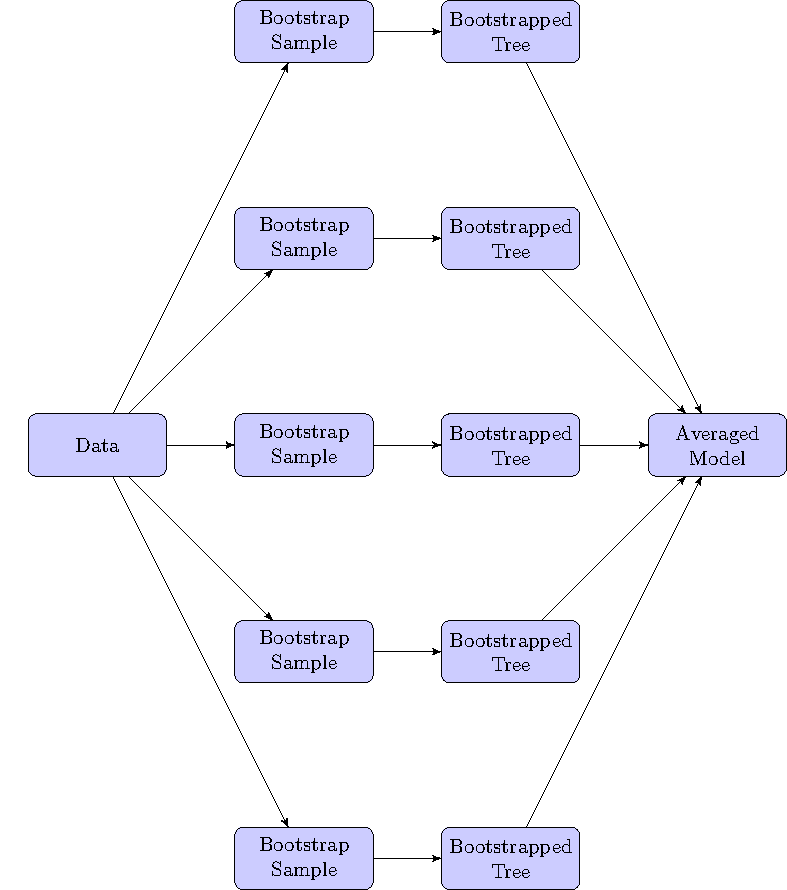
\includegraphics[width=0.5\textwidth]{reportcharts/boostrapflow.pdf}
    \caption{Flow of Bagging/Random Forests}
    \label{fig:boostrapflow}
\end{figure}
\begin{figure}
    \centering
    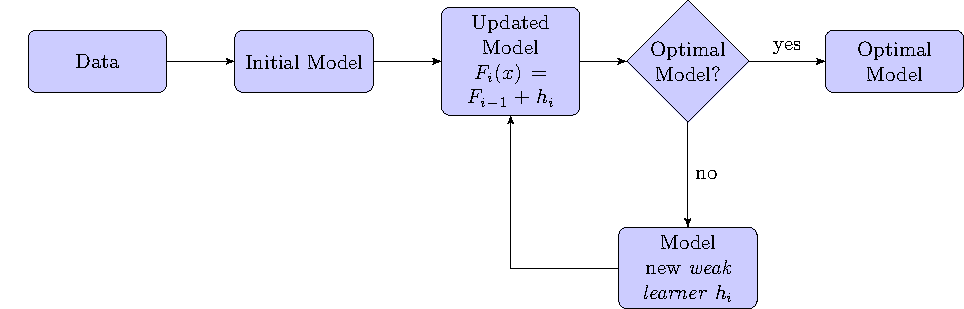
\includegraphics[width=0.5\textwidth]{reportcharts/boostingflow.pdf}
    \caption{Flow of Boosting}
    \label{fig:boostingflow}
\end{figure}


\section{Bagging/Random Forests}
\subsection{Bagging}
\textbf{B}ootstrap \textbf{Agg}regat\textbf{ing} (Bagging) \cite{bagging} uses multiple learning samples from the $\{x_{i}, y_{i}\}_{i=1}^{n}$ dataset, we collectively denoted these as $\mathcal{L}$. 
We denote each bootstrap sample as $\mathcal{L}_k$ where $k \in [1, \dots, B]$.
\medskip\\
{\color{gray} \textbf{Aside:} The paper was written by Leo Breiman who invented CART and edited by Ross Quinlan who invented ID3}
\medskip\\
The aim here is to get an aggregated predictor, made up of individual predictors $\varphi_k$ which is better than the individual predictor, which we will denote the final predictor as $\varphi$, defined as:
\begin{equation}
    \varphi = \frac{1}{B} \sum_{k=1}^{B} \varphi_k
\end{equation}

\subsubsection{Bagging Algorithm}
Here we present the Classification Algorithm (The Regression Algorithm is similar but adjusted accordingly for non-categorical data):
\begin{algorithm}
\begin{enumerate}
    \item A seed is set to allow for replication
    
    \item The full dataset is split \textit{randomly} into a learning set $\mathcal{L}$ and a testing set $\mathcal{T}$
    
    \item A Classification Tree is constructed from the full $\mathcal{L}$ and the test set $\mathcal{T}$ is run to test the misclassification rate
    
    \item 50 bootstrap sample from $\mathcal{L}$ are drawn randomly, and each make a $\phi$ classifier to form $\phi_1, \dots, \phi_{50}$
    
    \item All 50 $\phi$ classifiers are compared with each other and the most common classifier is selected, else, the class with the lowest error relative to the full Classification Tree is selected and this becomes $\varphi_k$
    
    \item Repeat steps 4-5 $k$ times and average the $\varphi_k$ values to obtain $\varphi$
\end{enumerate}
\caption{Classification Bagging}
\end{algorithm}\\
One can implement this algorithm using the {\color{blue} \texttt{ipred}} library in {\color{blue} \texttt{R}}

\subsection{Random Forests}
Random Forests are a natural development from Bagging as they use very similar techniques for growing ensembles. 
In Breiman's paper \textit{Random Forests} \cite{randomforest}, which will be replicated here, he noted that while both Bagging and Random Forests are similar, Bagging is akin to ``\dots darts thrown at random boxes \dots", Random Forests are much more civilized in nature as they are formed by voting ``\dots for the most popular class."
\medskip\\
We begin by using Breiman's definition of what a Random Forest is \cite{randomforest}:
\begin{definition}[Random Forests]
    A tree-based method formed from $k$, $k \in \mathbb{N}$, independent and identically distributed ensemble of classifiers, $h_1, \dots , h_k$.\\
    Each tree casts one vote for the most popular class which is to be selected.
\end{definition}

\subsubsection{Random Forest Algorithm}
Using the above definition, we can adapt the Bagging Algorithm into a Random Forest Algorithm with some minor changes as below
\begin{algorithm}
\SetAlgoLined
\begin{enumerate}
    \item A seed is set to allow for replication
    
    \item Draw $B$ bootstrapped samples from the learning set $\mathcal{L}$
        
    \item Grow a random forest as follows:
    \begin{enumerate}
        \item Select $m$ variables randomly from the sample $\mathcal{L}_b$ where $b \in [1, \dots, B]$
        
        \item Form a regular decision tree using only the selected features and the relevant metric described above
        
        \item Output the classifiers $\phi_1, \dots, \phi_B$
    \end{enumerate}
    
    \item Make a prediction as follows
    \begin{description}
        \item[Regression] $ \frac{1}{B} \sum_{b=1}^{B} \phi_b $
        
        \item[Classification] $majority \{\phi_b\}_{b=1}^{B}$
    \end{description}
\end{enumerate}
\caption{Random Forest Algorithm}
\end{algorithm}
Here, we note the following when choosing the preferred optimal value of $m$ (For which the library used for implementation, {\color{blue} \texttt{randomForest}}, does this automatically if undefined by the user):
\begin{itemize}
    \item \textbf{Classification} - $m = \left \lfloor{\sqrt{p}} \right \rfloor$ with minimum node size one
    
    \item \textbf{Regression} - $m = \left \lfloor{\frac{p}{3}} \right \rfloor$ with minimum node size five
\end{itemize}

\subsection{Out of Bag Samples}
The \textbf{Out of Bag Samples} (OOB) is used to check how good how well a model is fitted. 
A feature of selecting only a certain sample for bootstrapping is that we can use the samples not selected for a certain bootstrap to be a testing variable. 
Thus if variable $\{x_i, y_i\} \notin \mathcal{L}$ we can construct a predictor for this variable from the trees in which this variable is not a training data in.
\medskip\\
We are able to use this value to tell us right away if a model is good as a good model would have a low OOB value. 
This is helpful as {\color{blue} \texttt{R}} calculates the OOB value for us automatically and if a bad model were to be found to have been fitted, we can discover this early on before proceeding onwards towards predicting values.

\subsection{A Note on Implementation}
One can see from these algorithms that Bagging and Random Forests are very similar. 
In fact, one can see from the algorithm for Random Forests that if one sets $m = p$, which means all variables are selected in this Random Forest, one is practically performing Bagging.
Thus we have that \textbf{Bagging} $\subset$ \textbf{Random Forest}.
\medskip\\
When implementing this in {\color{blue} \texttt{R}}, one can use this fact to reduce the number of libraries loaded into {\color{blue} \texttt{R}}.
Here, instead of using {\color{blue} \texttt{ipred}}, one can instead use {\color{blue} \texttt{randomForest}} setting \texttt{mtry = p}, where $p$ is the number of variables one has in the training dataset.
One finds that there is no substantial difference between these two methods, besides sampling bias which one always expects to occur when bootstrapping.



\section{Boosting}
While the previously seen methods of Bagging and Random Forests work on Bootstrapping samples and running many trees at the same time before aggregating/voting for results, Boosting involves using many ``weak learners" which learn from incorrect predictions. 
Here, incorrect learners are sampled more often and given more weight when learning to improve on these mistakes and try to minimize the errors that these weak learners produce.
The final model is formed from combining all the weak learners into a much stronger single model.

\subsection{AdaBoost}
The first popular boosting algorithm is \textbf{Ada}ptive \textbf{Boost}ing \cite{adaboost} (AdaBoost). 
AdaBoost uses $t = [1,\dots,T]$ \textit{weak learners}, made up of small one-step decision trees which individually are not accurate, but which combined makes a much better model.
\medskip\\
AdaBoost gives a weight $w_t (i)$ to each predictor $x_i$ to help decide which variable to focus on after each iteration.
A predictor which has been {\color{red} \underline{incorrectly classified}} previously is given more weighting in subsequent weak learners compared to previous weak learners.

\subsubsection{Weak Learners}
We have a weak hypothesis $h_t : X \rightarrow \{-1,+1\}$ for $x_i \in X$.
How good the hypothesis is can be tested by its error $\varepsilon_t$.
\begin{equation}
   \varepsilon_t = \sum_{h_t (x_i) \neq y_i} w_t (i) 
   \label{eq:weaklearn}
\end{equation}
In computations there exists a function called \textbf{WeakLearn} which achieves this by using \textit{decision stumps}.

\subsubsection{AdaBoost Algorithm for Classification}
Combining the above, we can now generate the AdaBoost Algorithm as follows:
\begin{algorithm}
\SetAlgoLined
\begin{enumerate}
    \item Set $\textbf{w}_1 = \frac{1}{n}$ $\forall$ $n$ training sets
    
    \item \For{$t = 1,\dots,T$}{
    Pick $h_t$ which minimizes $\varepsilon_t = \sum_{h_t (x_i) \neq y_i} w_t (i) $ \\
    Compute weight of chosen classifier 
    \[\alpha_t = \frac{1}{2} \log \frac{1 - \varepsilon_t}{\varepsilon_t} \] \\
    Update weights
    \[ w_{t+1} (i) = \frac{w_t (i) \exp{-\alpha y_i h_t (x_i)}}{Z_t} \]
    Where $Z_t$ is the normalization factor \\
    Break if $\varepsilon_t = 0$ or $\varepsilon_t \geq \frac{1}{2}$
    }
    
    \item Output final hypothesis
    \[ h_f (x) = \text{sign} \left(\sum_{t=1}^T \alpha_t h_t (x) \right) \]
\end{enumerate}
\caption{AdaBoost}
\end{algorithm}

\subsubsection{AdaBoost for Regression}
The algorithm and mathematics behind AdaBoost for regression work similarly to above. Refer to \cite{adaboost} to see the AdaBoost Algorithm for Regression.

\subsubsection{AdaBoost is a Random Forests}
A conjecture noted by Breiman in \textit{Random Forests} \cite{randomforest} was that both AdaBoost and Random Forests are so similar that they are essentially equivalent.

\subsection{Gradient Boosting}
A more generalized version of AdaBoost came along in 1999 by Jerome Friedman (The second author in CART) in \textit{Greedy Function Approximation: A Gradient Boosting Machine} \cite{gbm}.
Here, we maintain the idea of using \textbf{Weak Learner} from AdaBoost while introducing two further components:
\begin{description}
    \item[Loss Function] - A function to estimate how good a model performs
    
    \item[Additive Model] - The method of adding Weak Learners to each other one at a time
\end{description}
This can be summarised into three simple steps:
\begin{enumerate}
    \item An initial model $F_0$
    
    \item A new model $h_1$ is fitted based on the errors of the previous model - this is the weak learner
    
    \item The previous model and the weak learner are combined to get an updated model $F_1 (x) = F_0 (x) + h_1 (x)$
\end{enumerate}
These three steps are repeated for $m$ until the errors have been minimized as much as possible which gives us the following iterative steps:
\[
\begin{array}{ccc}
    F_1 (x) & = & F_0 (x) + h_1 (x) \\
    F_2 (x) & = & F_1 (x) + h_2 (x) \\
    \vdots & \vdots & \vdots \\
    F_m (x) & = & F_{m-1} (x) + h_m (x)
\end{array}
\]
The final goal here is to find an approximate $\hat{F} \approx F_m (x)$ which minimize the the expected loss function which would minimize the bias of the final model.
\[
\hat{F} = \argminB \EX [L(y,F(x)]
\]
We will introduce this in a more general sense before showing how Tree-Based Methods can be fitted and used.

\subsubsection{Loss Function}
To start, we need to establish $F_0 (x)$.
Here, we establish a function which minimizes the cost function as such:
\begin{equation}
    F_0 (x) = \argminB_\gamma \sum_{i=1}^{n} L(y_i, \gamma)
\end{equation}
We will use a method called \textbf{gradient descent} to estimate the loss function.

\subsubsection{Gradient Descent}
Gradient Descent, also referred to as \textit{steepest-descent}, is a method to find a local minimum of a function. 
It is one of the simplest minimization methods used and is great for boosting as we will be applying this method each time you grow a tree.
One defines the gradient descent for boosting as follows:
\begin{equation}
    g_m (x) = \left[ \frac{\partial L(y,F(x))}{\partial F(x)} \right]_{F(x) = F_{m-1} (x)}
\end{equation}
Friedman found that the best loss function is $-g_m (x)$, which can be referred to as the ``pseudo-responses" $\Tilde{y}_m$ \cite{gbm}.
One uses the responses from $\Tilde{y}$ to fit a weak learner $h_m$ onto it.

\subsubsection{Scaling Multiplier}
The last value one needs to find $\gamma_m$ when updating the model is a multiplying scaling factor $\rho_m$ which gives us the optimal steepest-descent value when updating the model:
\[ \gamma_m = \rho_m h_m (x) \]
where $\rho_m$ is the following:
\begin{equation}
    \rho_m = \argminB_\gamma \sum_{i=1}^{n} L (y_i, F_{m-1} (x) + \gamma h_m (x))
\end{equation}
Intuitively, this scales each weak learner so that it leads to \underline{minimal} changes to the model while correcting previous errors, which is the intent of a weak learner.
One can finally solve for $F_m (x)$ using the iterative model
\begin{equation}
F_m (x) = F_{m-1} (x) + \rho_m (x)
\label{eq:learner}
\end{equation}

\subsubsection{Adjustment for Trees}
An issue with the current method of construction is that we end up losing the disjoint regions that Decision Trees give when combining two separate models. 
Having written both CART \cite{tree} and \cite{gbm}, Friedman knew of this and suggested the following, noting that the additive form of Decision Trees, following Friedman, are as follows:
\[
h(x;\{b_j,R_j\}_{1}^{J}) = \sum_{j=1}^{J} b_j \mathds{1} (x \in R_j )
\]
For disjoint regions $\{R_j\}_{1}^{J}$ and base learner parameters $\{b_j\}_{1}^{J}$ with an indicator function $\mathds{1} (x \in R_j)$ to indicate whether predictor $y_i$ is in the region or not.
Since each region in each tree is disjoint, if $x \in R_j$ then $h(x) = b_j$.\\
Thus one can update \ref{eq:learner} to become:
\begin{equation}
\begin{split}
    F_m (x) &= F_{m-1} (x) + \rho_m \sum_{j=1}^{J} b_{jm} \mathds{1}(x \in R_{jm}) \\
    &= F_{m-1} (x) + \sum_{j=1}^{J} \gamma_{jm} \mathds{1}(x \in R_{jm})
\end{split}
\end{equation}
From here, one can establish the Gradient Boosting Algorithm adapted for Tree-Based learners.

\subsubsection{Gradient Boosting Algorithm}
Combining all the processes above together, we achieve the following algorithm for Tree-Based Boosting. 
We will show the case for the Regression Algorithm although one can easily manipulate this for Classification if one encodes categorical variables numerically.
\begin{algorithm}
\SetAlgoLined
\begin{enumerate}
    \item Set $F_0 (x) = \argminB_\gamma \sum_{i=1}^{n} L(y_i, \gamma)$
    
    \item \For{$m = 1,\dots,M$}{
    Compute 
    \[g_m (x) = - \left[ \frac{\partial L(y_i,F(x_i))}{\partial F(x_i)} \right]_{F(x) = F_{m-1} (x)} \] \\
    Fit $h_m$ to $g_m$ to obtain nodes $\{R_{jm}\}_{1}^{J} $ \\
    Compute multiplier $\gamma_{jm}$ \\
    Set 
    \[ F_m (x) = F_{m-1} (x) + \sum_{j=1}^{J} \gamma_{jm} \mathds{1}(x \in R_{jm})
    \]
    }
    
    \item Output $F_m$ as our $\hat{F}$ model
\end{enumerate}
\caption{Gradient Boosting}
\end{algorithm}\\
We need to find an initial loss function which is easy to calculate. 
In the regression setting, one finds that setting $F_0 = median \{y_i\}_{1}^{n}$ is the easiest and most effective starting point, although others do exist.
\medskip\\
\textbf{Note}: One can see that this algorithm does not implement well in a classification setting and especially using Classification Trees.
In \cite{gbm}, the method recommended is to use Logistic Regression and log-likelihood functions. 
This is able to simulate regression, by nature of Logistic Regression, but allow us to carry classification.
One can also just run the classification as a Regression Tree and then round the final estimator to achieve a classification prediction although this really only works up to a certain extent and is not as accurate as just using Logistic Regression for classification here.
  
\subsection{xgBoost}
\textbf{Extreme Gradient Boosting}, referred to as xgBoost, \cite{xgboost} is a modern implementation of Gradient Boosting which applies Gradient Boosting as a ``scalable machine learning system for tree boosting" \cite{xgboost}.
\medskip\\
The biggest difference between both methods is that xgBoost uses the \underline{Second-Order} derivative of the Loss Function, i.e. differentiate twice instead of once.
The idea here is to find more information about the loss more quickly than previous implementations.
\medskip\\
Another difference between regular boosting introduced in \textit{Greedy Function Approximation} \cite{gbm} and xgBoost was the idea of \textbf{Stochastic Boosting} introduced in Friedman's follow up \textit{Stochastic Gradient Boosting} \cite{stochasticgb}.
Here, one sub-samples rows and columns before creating each tree. 
According to Chen ``Using column sub-sampling prevents over-fitting more so than traditional row sub-sampling". 
\medskip\\
A final aspect is the use of L1 or L2 regularization on the leaf weights to further avoid over-fitting.

\subsubsection{Second-Order Approximation}
One can define the Second-Order approximation of the loss function to be, following \cite{xgboost}, we start with the loss function we want to minimize:
\begin{equation}
    L = \sum_{i=1}^{n} L(y_i,F_{m-1} (x_i) + f_t (x_i)) + \Omega (f_t)
\end{equation}
Then, expanding by Taylor and simplifying, one can find an approximate to the Second-Order differential to be:
\begin{equation}
    L \approx \sum_{i=1}^{n} \left[g_i f_t (x_i) + \frac{1}{2}h_i f_t^2 (x_i) \right] + \Omega (f_t)
\end{equation}
where $g_i = \partial_{\hat{y}^{(t-1)}} l(y_i,\hat{y}^{(t-1)})$ and $h_i = \partial_{\hat{y}^{(t-1)}}^2 l(y_i,\hat{y}^{(t-1)})$.
\medskip\\
Set $\Omega (f_t) = \gamma T + \frac{1}{2} \lambda \sum_{j=1}^{T} w_j^2$, where $w_j$ is the weight of the leaf $w_j = -\frac{\sum g_i}{\sum h_i + \lambda}$ and one can calculate the loss function we want as,
\begin{equation}
    \Tilde{L} = -\frac{1}{2} \sum_{j=1}^{T} \frac{\left(\sum g_i\right)^2}{\sum h_i + \lambda} + \gamma T
\end{equation}
One can now approximate the loss reduction of the split by setting \texttt{Gain = Loss Before - Loss After} which is,
\[
L_{split} = \frac{1}{2} \left[ \frac{\left(\sum_{i \in {I_L}} g_i\right)^2}{\sum_{i \in {I_L}} h_i + \lambda} + \frac{\left(\sum_{i \in {I_R}} g_i\right)^2}{\sum_{i \in {I_R}} h_i + \lambda} -\frac{\left(\sum_{i \in I} g_i\right)^2}{\sum_{i \in I} h_i + \lambda} \right] - \gamma
\label{eq:secndorderl}
\]
One can now use \ref{eq:secndorderl} and implement it with the Gradient Boosting Algorithm above and achieve xgBoost.


\chapter{Optimizing Trees}
While both Random Forests and Boosting are very accurate predictors, they achieve this by sacrificing interpret-ability. 
This makes it harder to show how each decision is made and is the trade-off necessary in order to achieve higher accuracy. We now return to Decision Trees but under a more modern light using ideas from operations research as a basis for the algorithm.



\section{Trees as an Optimization Problem}
Improvements in technology have now allowed us to look at decision trees under a different perspective.
Previously, the most efficient way to improve accuracy without inducing bias is to look at improving the metrics used for splitting and then when the limits have been pushed, use ensemble techniques to aggregate and minimizing the errors.\\
Dimitris Bertsimas and his PhD student, Jack Dunn proposed reforming decision trees as an optimization problem \cite{oct}. 
This is actually a realisation of Leo Breiman's dream to solve the entire decision tree in one go.
In fact, in CART, Breiman noted the following \cite[p.42]{BreimanDT} in his book:
\bigskip\\
\say{\textit{Finally, another problem frequently mentioned (by others, not by us) is that the tree procedure is only one-step optimal and not overall optimal. ...If one could search all possible partitions ...the two results might be quite different.
This issue is analogous to the familiar question in linear regression of how well the stepwise procedures do as compared with ‘best subsets’ procedures. We do not address this problem. At this stage of computer technology, an overall optimal tree growing procedure does not appear feasible for any reasonably sized dataset.}}
\bigskip\\
Thus, really we should now look at the problem as a Mixed-Integer Optimization Problem (MIO).
Revisiting CART, we can now look at this as a programming problem called the \textbf{Optimal Tree Problem}.

\subsection{What is Mixed-Integer Optimization}
\textbf{Mixed-Integer Programming} is a subset of Integer Programming where only some of the variables have integer constraints whereas others are more free and can be non-integers within the constraints.
While the idea had been conceived by Kantorovich and, independently, Dantzig, it was not until 1981 \cite{arthanaridodge} that more attempts to tackle statistical problems took flight.
Even then, it took until 2004 \cite{bixby} when optimizing the Mixed-Integer Programming problem became possible. 
Fortunately, in the past decade, a modern MIO solver in  {\color{blue} \texttt{Gurobi}} \footnote{https://www.gurobi.com/resource/mip-basics/} had been introduced which allow us to solve many Mixed-Integer problems more efficiently.
\medskip\\
The method to solve these Mixed-Integer problems is call \textbf{Branch and Bound} first introduced in the \textit{Travelling Salesman Problem} \cite{travellingsalesman}. 
In simple terms, one starts by ``relaxing" the problem with no integer restrictions, and solving it using normal linear programming methods to see if the constraints we have relaxed end up being integer solutions anyways.
Normally, this is not the case and so we pick one constraint and split the problem into two sub-problems with tighter constraints where, for example, if the value for variable $x$ in linear programming ``relaxation" is 4.6, then we impose constraints $x \leq 4$ and $x \geq 5$ the next time we run linear programming.
The full algorithm can be found in \cite{travellingsalesman} and has been skipped on purpose here for conciseness.
\medskip\\
{\color{brown} In this instance, the software we use {\color{blue} \texttt{Interpretable AI}} has its own implementation of {\color{blue} \texttt{Gurobi}} already built in}

\subsection{CART as a Linear Problem}
Given a complexity parameter $\alpha$ which controls the tradeoff between accuracy and complexity, a minimum number in each node $N_{min}$ and a dataset $\{x_i, y_i\}_{i=1}^{n}$ we aim to solve the problem $\forall \ l$ leaf nodes $ \in T$ tree:
\[ \begin{array}{cc}
        \min  & R(T) + \alpha \left|T\right|\\
        \text{s.t.}  & N(l) \geq N_{min}
    \end{array} \]
Where $N(l)$ is the number of points in leaf node $l$ and $R(T)$ is the misclassification error from before.

\section{The Optimal Classification Tree}
We now proceed on to the Optimal Classification Tree \cite{oct}.
Here, we attempt to solve the tree as a MIO problem which allows us to avoid having to choose whether to branch and what variable we would branch on.
In this way, we are able to create the model in one go and avoid the decision making process which leads to the heuristically greedy nature of CART.\\
\textbf{Note}: We now follow the method presented by Jack Dunn in his thesis which, in turn, was published in \cite{oct} which you may refer to for further details.

\subsection{Growing the Tree}
To formulate this tree, we note that the maximal tree we can grow at depth $D$ contains $T = 2^{(D + 1)} - 1$ nodes, which we will denote as $t = 1,\dots,T$. Now, we need the following notations.
We denote for node $t$, $p(t)$ as the parent node and $A(t)$ any ancestor node of $t$. We then group all nodes into two sets as follows:
\begin{enumerate}
    \item \textbf{Branch Nodes} - The nodes $t \in T_B = \{1,\dots,\left \lfloor{\frac{T}{2}} \right \rfloor \}$ which apply the split in the form of a matrix $\mathbf{a}^\intercal \mathbf{x} < b$
    
    \item \textbf{Leaf Nodes} - The nodes $t \in T_L = \{\left \lfloor{\frac{T}{2}} \right \rfloor + 1, \dots, T$ which make predictions
\end{enumerate}
The split at node $t \in T_B$ corresponds to the variables $\mathbf{a}_t \in \mathbb{R}^n$ and $b_t \in \mathbb{R}$ and set both $\textbf{a}_t = b_t = 0$ when we no longer want to split (Forcing all nodes down one branch) for computational reasons.
To track which nodes were split on, an indicator variable $d_t = \mathds{1}$ which gives an output of $1$ when a node is split.
The following constraints can be applied:
\begin{align}
     a_{jt} \in \{0,1\}, & j=1,\dots,p, & \forall \ t \in T_B \label{eq:octconditions1}\\
    0 \leq b_t \leq d_t, & & \forall \ t \in T_B & \label{eq:octconditions2}\\
    \sum_{j=1}^{p} a_{jt} = d_t, & & \forall \ t \in T_B & \label{eq:octconditions3} 
\end{align}
A final constraint $d_t \leq d_{p(t)}$, $\forall \ t \in T_B P \backslash \{1\}$ is added so that a branch node does not split if the parent node does not also split.

\subsection{The Mixed-Integer Optimization Problem}
Using the constraints listed above, we can now model the tree using Mixed-Integer Optimization.
At each step we will keep track of what is being assigned to each leaf node.
We have an indicator variable $z_{it} = \mathds{1}\{\textbf{x}_i \text{ in node } t\}$ with $\sum_{t} z_{it} = 1$ tracking what is assigned to each node and $l_t = \mathds{1}\{\text{leaf } t \text{ contains any points}\}$ to enforce $N_{min}$ so that:
\begin{align}
       z_it \leq l_t, & \ t \in T_B \label{eq:octrestrictions1}\\
    \sum_{i=1}^{n} z_it \geq N_{min} l_t, & \ t \in T_B \label{eq:octrestrictions2} 
\end{align}
Which now allows us to formulate the tree splits, where $i = 1,\dots,n$, $\forall \ t \in T_B$ as thus:
  \begin{align}
    \mathbf{a}_m^\intercal \mathbf{x}_i < b_t + M_1 (1 - z_{it}),  & \ \forall \ m \in A_L (t), \label{eq:octlt}\\
    \mathbf{a}_m^\intercal \mathbf{x}_i \geq b_t - M_2 (1 - z_{it}), & \ \forall \ m \in A_R (t), \label{eq:octgeq}  
  \end{align}
\textbf{Note:} In practice, the strong inequality \ref{eq:octlt} is not computationally feasible and so often a small, but computationally significant, error term $\epsilon$ is used to combat this.
\medskip\\
From the constraints, we can also solve the constants $M_1$ and $M_2$ which lead to the following inequalities which can be used by MIO when formulating the tree splits $\forall \ t \in T_L$:
  \begin{align}
    \mathbf{a}_m^\intercal (\mathbf{x}_i + \epsilon) \leq b_t + (1 + \epsilon) (1 - z_{it}),  & \  \forall \ m \in A_L (t), \label{eq:finoctleq}\\
    \mathbf{a}_m^\intercal \mathbf{x}_i \geq b_t - (1 - z_{it}), & \ \forall \ m \in A_R (t), \label{eq:finoctgeq}  
  \end{align}

\subsubsection{Labelling Incorrect Predictions}
To keep track of what each predictor gives out as a prediction, we need to find a way to keep track of what we have misclassified.
Lets say we have a matrix $Y$, we note the following cost of an incorrect label prediction to the algorithm for $i = 1,\dots,n$ and $k = 1,\dots,K$:
\[
Y_{ik} = 
\begin{cases}
1, & \text{if } y_i = k\\
-1, & \text{otherwise}
\end{cases}
\]
Setting $N_t$ to be the total number of points in node $t$ and $N_{kt}$ the number of those labelled $k$ in node $t$, we also get,
\begin{equation}
    N_t = \sum_{i=1}^{n} z_{it}, \ \forall\ t \in T_L
    \label{eq:octnt}
\end{equation}
\begin{equation}
    N_{kt} = \frac{1}{2}\sum_{i=1}^{n} (1 + Y_{ik}) z_{it}, \ \forall\ t \in T_L
    \label{eq:octnkt}
\end{equation}
Thus, the optimal label $c_t$ can be defined as:
\[
c_t = \argmaxB_{k=1,\dots,K} N_{kt}
\label{eq:optimallabel}
\]
where we find that the predictor will contain these points at each leaf node,
\begin{equation}
\sum_{k=1}^{K} c_{kt} = l_t, \ \forall \ t \in T_L
\label{eq:octcontainpoints}
\end{equation}


\subsubsection{Optimal Loss}
Knowing the above, we can now find the optimal loss at each node $L_t$ as,
\[
L_t = N_t - \max_{k=1,\dots,K} N_{kt}
\]
Which can be linearized $\forall \ t \in T_L$ as,
\begin{align}
    L_t &\geq N_t - N_{kt} - M(1 - c_{kt}), & k=1,\dots,K \label{eq:octmiscl1}\\
    L_t &\leq N_t - N_{kt} + M c_{kt}, & k=1,\dots,K \label{eq:octmiscl2}\\
    L_t &\geq 0, &  \label{eq:octmiscl3}
\end{align}
For any sufficiently large $M$.

\subsection{The OCT Model}
One can note from above that what we aim to do is to minimize the total misclassification cost as well as the complexity of the tree. 
We have a baseline model with accuracy $\hat{L}$ to normalize against and thus, for an independent $\alpha$ one has,
\begin{equation}
    \min \frac{1}{\hat{L}} \sum_{t \in T_L} L_t + \alpha \sum_{t \in T_B} d_t
    \label{eq:OCTmodel}
\end{equation}
Which is the OCT Model which has the restraining conditions, \ref{eq:octconditions1}, \ref{eq:octconditions2}, \ref{eq:octconditions3}, \ref{eq:octrestrictions1}, \ref{eq:octrestrictions2}, \ref{eq:finoctgeq}, \ref{eq:finoctleq}, \ref{eq:octnt}, \ref{eq:octnkt}, \ref{eq:octcontainpoints}, \ref{eq:octmiscl1}, \ref{eq:octmiscl2}, \ref{eq:octmiscl3}.

\subsubsection{Warm Starts}
Dunn noted in Optimal Classification Trees \cite{oct} that a ``Warm Start" provides a benefit in the way of reducing run time of the algorithm. Please refer to section 2.3 of \cite{oct} for further details.

\subsection{Optimal Classification Tree Algorithm}
We can now implement the MIO problem as an algorithm:
\begin{algorithm}
\SetAlgoLined
\begin{enumerate}
    \item Set a maximal depth $D_{max}$ and a minimum leaf size $N_{min}$
    
    \item For $D = 1,\dots,D_{max}$, for $C = 1,\dots,2^D - 1$:
    \begin{enumerate}
        \item Run CART with $N_{min}$ and $\alpha = 0$ to get an initial solution
        
        \item Choose the warm start with the lowest error
        
        \item Use selected warm start to solve the MIO problem
        
        \item Add solution to warm start pool
    \end{enumerate}
    \item For any value of $\alpha$, remove all non-optimal solutions
    
    \item Select the best performing solution and the $\alpha$ for which this solution is optimal
\end{enumerate}
\caption{Optimal Classification Tree}
\end{algorithm}



\section{An Extension to Hyper-planes}
The nature of CART makes it very difficult to try to introduce hyper-planes when splitting data sets. 
Previous attempts have been made by Wei-Yin Loh at the University of Wisconsin-Madison \cite{fact}, however, these have not been commonly used.
\medskip\\
An interesting nature of using Mixed-Integer Programming is that you are no longer restricted to linear splits within categories. 
By adjusting a few of the constraints, such as redefining the cost-complexity parameter to work across splits, we have put on the OCT Model, one can apply the same method but on hyper-planes between variables. 
More can be found in \cite{oct}.
\medskip\\
An example of a Optimized Tree with Hyper-planes is seen in fig \ref{fig:octhyp}.
\begin{figure}
    \centering
    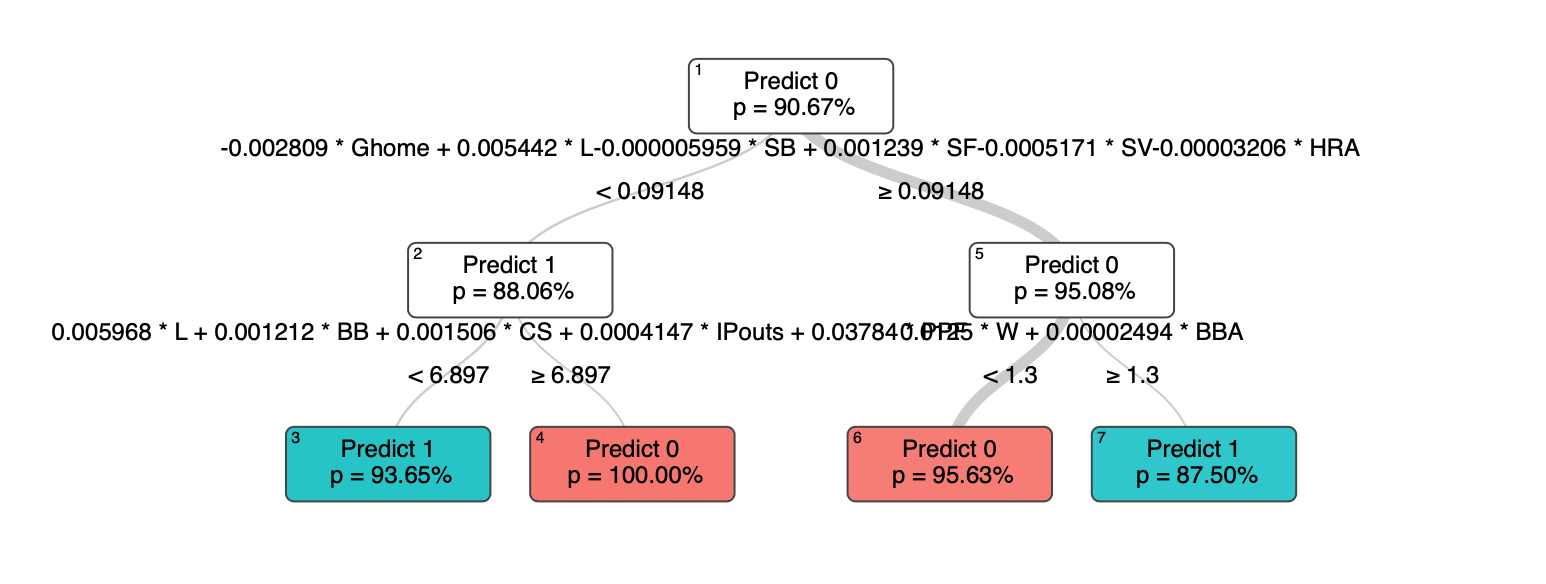
\includegraphics[width = 10cm]{reportcharts/octhyp.png}
    \caption{OCT with Hyper-Plane}
    \label{fig:octhyp}
\end{figure}\\
One can see that we essentially form a linear regression model and splitting upon the results.
While useful for very large data sets, this will be as far as we go for this dataset.


\section{Comparing OCT with Bagging}
While OCT solves many issues regarding accuracy while maintaining interpretability, it is a good idea to check and see if we can, in turn, bootstrap OCT and produce a much more accurate model than previously possible.
In this case, we will be comparing it with the regular OCT model to see how well bagging improves the accuracy score of the test.

\subsection{Bagging OCT}
To perform this bagging, we create a \texttt{for} loop to generate 100 new samples which are then fitted and a prediction is based on the same data is made for each run.
We store the score of each run and average them all to create a final predictor similar to how {\color{blue} \texttt{ipred}} achieves this.
The following results were achieved and shown in tables \ref{tab:octbag} and \ref{tab:octauc}:
\subsubsection{Table of results for comparison}
Tables \ref{tab:octbag} and \ref{tab:octauc} show us how well our bagged model does in comparison with the base model.
\begin{table}
    \centering
    \begin{tabular}{|c|c|}
        \hline
        \textbf{Model Type} & \textbf{Accuracy Score} \\
        \hline
        Optimal Classification Tree & 0.9140363\\
        \hline
        Bagged OCT & 0.9120215\\
        \hline
        Cross Model Score & 0.967092\\
        \hline
    \end{tabular}
    \caption{OCT vs Bagged OCT}
    \label{tab:octbag}
\end{table}

\subsubsection{ROC Curves and AUC Scores}
\begin{table}
    \centering
    \begin{tabular}{|c|c|}
        \hline
        \textbf{Model Type} & \textbf{AUC Scores} \\
        \hline
        Optimal Classification Tree & 0.701825663192676 \\
        \hline
        Bagged OCT & 0.923786095034238 \\
        \hline
    \end{tabular}
    \caption{AUC Scores for OCT models}
    \label{tab:octauc}
\end{table}
One notices that the models are very similar to each other and only once one looks at the AUC score (Figure \ref{fig:octroc}) can one see that an improvement occurs when we bag a model.
\medskip\\
\textbf{Note:} The original OCT contains only 4 leaf nodes.
With the nature of how OCT is calculated using MIO's, when predicting probabilities, this will result in ``Return the probabilities of class membership predicted by a model for each point in the features" according to the IAI reference manual. 
Thus, one would only find 4 points on the leaf node, resulting in the interesting ROC curve that we observe.
However, since Bagging averages our probabilities, we are able to find many more probabilities and thus the ROC curve there will seem more natural

\begin{figure}
    \centering
    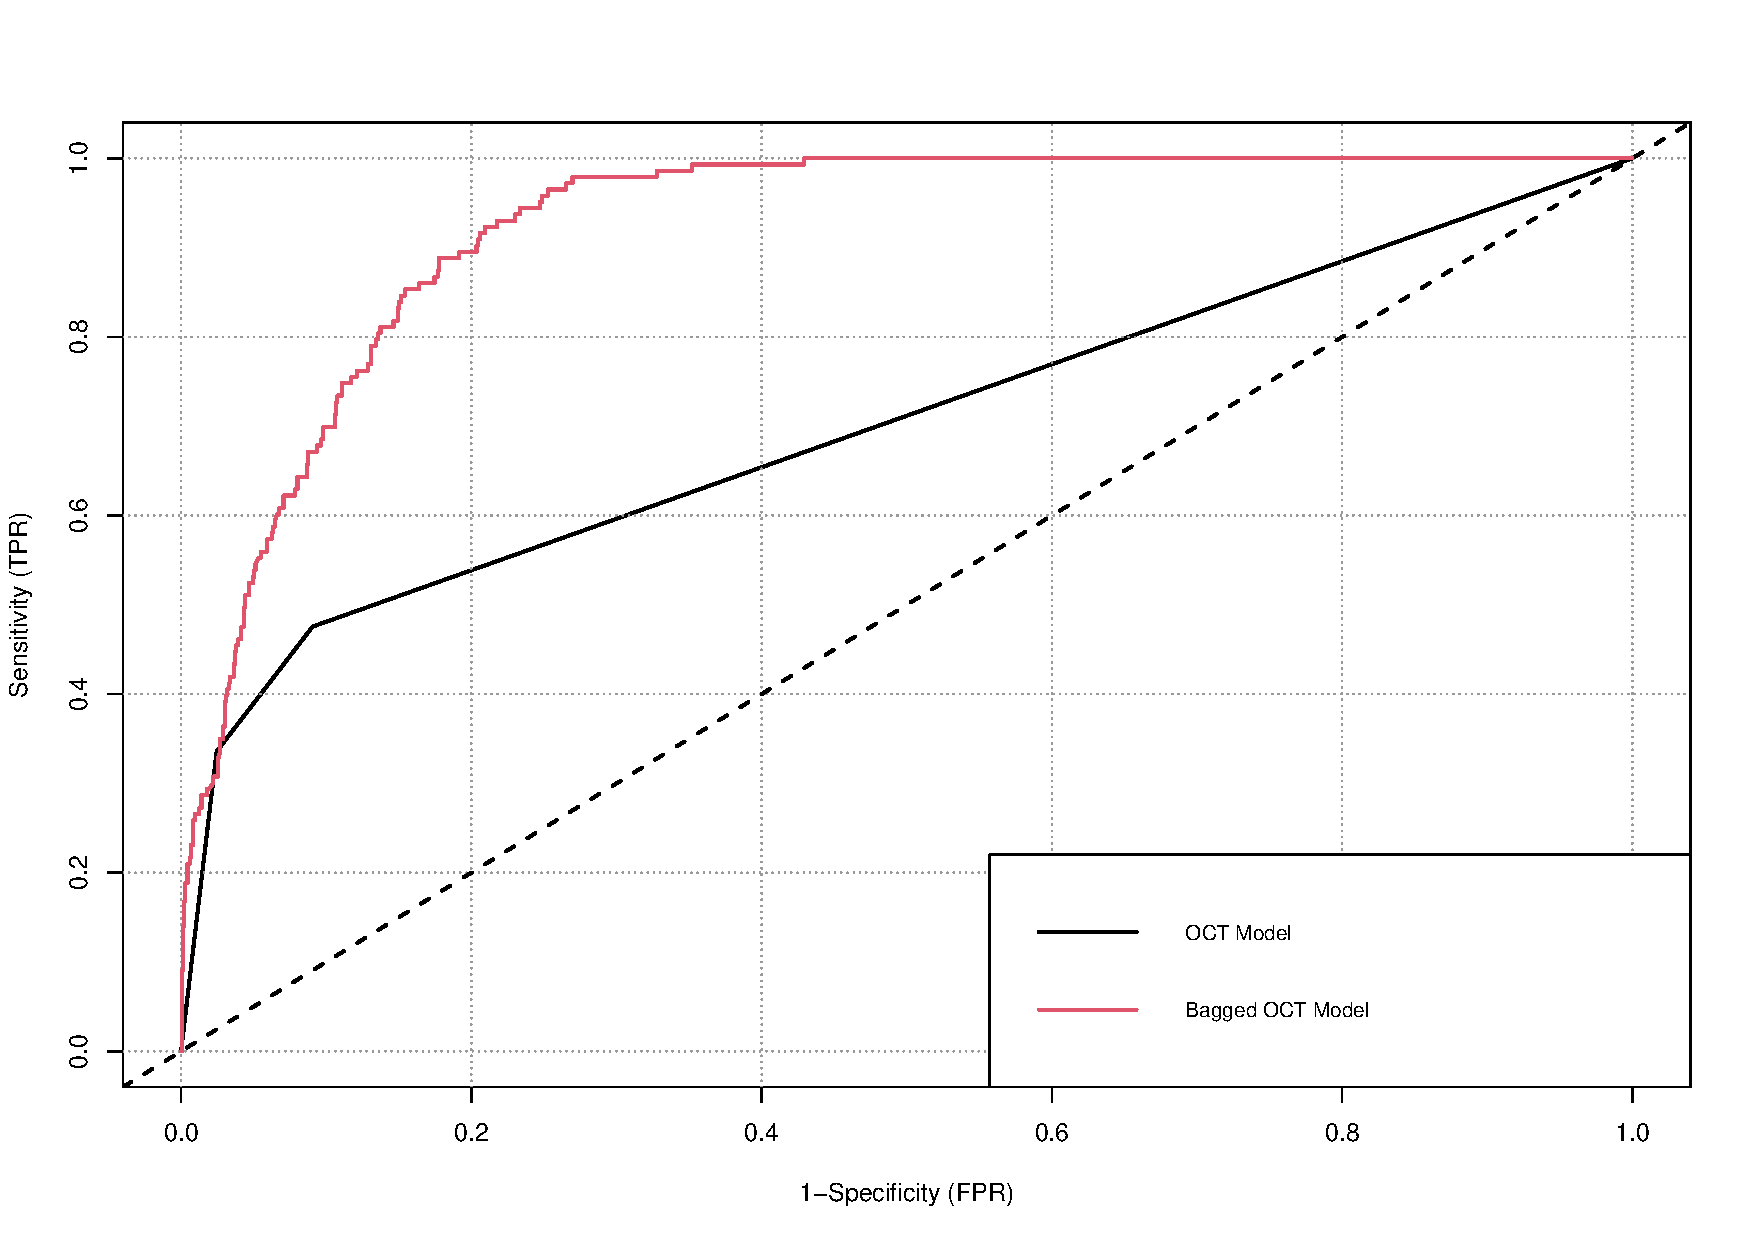
\includegraphics[width = 10cm]{reportcharts/octvbagged.pdf}
    \caption{ROC Curves comparing OCT with Bagged OCT}
    \label{fig:octroc}
\end{figure}

\section{Optimal Regression Trees}
Using similar techniques to Optimal Classification Trees, one can easily extend this to the Regression Trees using a few tweaks to the model.
In fact, most of the model remains the same as in the case for classification and it is only the labelling of incorrect predictions (not possible in regression) and loss function that needs changing.
Here, one follows \cite{octbook}, although an open source version would be Dunn's PhD thesis \cite{jackdunn}.

\subsection{The Optimal Regression Tree Problem}
One can reuse most of what we have previously seen here.
However, we must also look at how Regression Trees predict values to give us new restrictions.
From CART, we have that at each node, one prediction is made.
This can be modelled by a continuous variable $\beta_{0t}$.
Thus one can predict the variables $f_i$ using,
\[
f_i = \sum_{t \in T_L} \beta_{0t} z_{it}, \ \forall \ i \in n
\]
Which can be expressed as the following, $\forall \ i \in n$ and $t \in T_L$:
\begin{align}
    f_i &\geq \beta_{0t} - M_f (1 - z_{ik}) \label{eq:ortlin1} \\ 
    f_i &\leq \beta_{0t} + M_f (1 - z_{ik}) \label{eq:ortlin2}
\end{align}
\subsubsection{Regression Loss Function}
In the regression setting, our loss function is now the difference between the predicted value and the actual value.
In our case, \underline{either} the \textit{Absolute Loss} or the \textit{Squared Loss} can do just fine. 
Let us take the quadratic loss which linearly can be written as,
\begin{equation}
    L_i \geq (f_i - y_i)^2, \ \forall \ i \in n \label{eq:ortloss1}
\end{equation}

\subsection{ORT Model}
Now, one wants to minimize the loss that we achieve when building the model, so our new model is now:
\begin{equation}
    \min \frac{1}{\hat{L}} \sum_{i=1}^{n} L_i + \alpha \sum_{t \in T_B} d_t
    \label{eq:ortmodel}
\end{equation}
With restraining conditions \ref{eq:octconditions1}, \ref{eq:octconditions2}, \ref{eq:octconditions3}, \ref{eq:octrestrictions1}, \ref{eq:octrestrictions2}, \ref{eq:finoctgeq}, \ref{eq:finoctleq}, \ref{eq:octnt}, \ref{eq:octnkt}, \ref{eq:ortlin1}, \ref{eq:ortlin2}, \ref{eq:ortloss1}.

\subsection{Hyper-planes}
Similar to the case with classification, using MIO's one can now introduce hyper-planes to create decision boundarys.
Details can be found in \cite{octbook} and \cite{jackdunn} as per the case for ORT's.



\chapter{Application using Lahman Dataset}
Using data that we have put together (see Appendix), we are able to apply this to a real world scenario.
In this case, for Classification, we are trying to predict the likelihood that a baseball team would win their half of the league (Referred to as a Pennant and noted as \texttt{LgWin} in Lahman) at the end of the season given the statistics that they had achieved over the season. In this case, I am not considering how playoffs affect a teams chance of winning the league due to the randomness of playoffs and that we often find that the best team wins more often than not.
\medskip\\
By structure of Major League Baseball (MLB) we can efficiently create a training group based on the American League (AL) and test that with the National League (NL).
As both leagues essentially are independent of each other (baring inter-league play which only became prominent in the last couple of years) one can assume a relatively clean separation between training and testing data.
\medskip\\ 
Furthermore, we are able to collect data on players over an individual season as well as over an entire career. 
Each season's statistics is considered essentially independent of each other, however, it is possible for one to predict future performance based on past data.
\medskip\\
Often, some data exploration would have been performed to help decide what model one should be using.
This has been mostly skipped to save time although one can use the code provided in the appendix to perform their own exploration.
\medskip\\
\textbf{Note:} The data selected are not supposed to ``play nice" and thus we expect to have either a high bias or high variance. 
The Bias-Variance trade-off should come into play and we can see how each model performs when given more realistic data.

\subsection{How Decision Trees are used}
In modern baseball analytics, Decision Trees are one of the many methods used in evaluating performance for team construction. 
Many uses of Decision Trees are possible but we will be using only two usages in baseball.
This is a small glimpse into what is now referred to as \textbf{Sabermetrics}, although more casually, this is called \textbf{Moneyball} as a reference to Michael Lewis' book which looked into this very thing.

\subsubsection{Classification}
The Classification we are using would be predicting the likelihood of a team winning ``their" league.
In this case, we are using team season data to project how well a team has to perform to be considered a team which likely wins.
Individually, this usage seems arbitrary but it is in fact the first method a team uses when constructing teams as knowing how well a team has to do is invaluable to informing which players to target based on other models.
Our model here is a simplistic version used for a generic season, which unlike a realistic season, does not consider what other teams do as well. 
Further refinement of the model would be essential in this case, however, as a demonstration of application, it is not necessary for us to get into too much detail there.

\subsubsection{Regression}
An obvious example for a use of Regression Trees is predicting future salaries based on the previous seasons performance. 
In real life, salary raises and free agent contracts are often determined by last season's performance which are often used as a good predictor for next season's player output and value to the team.
\medskip\\
\textbf{Note:} Often for regression scenarios, one would first use \textit{linear regression} to see if the model can be easily fit as that is the simplest model we have.
Only after doing that would one try other methods such as the tree-based methods we present here.

\section{Playoff Prediction}
As previously noted, we can split data into two (\textbf{AL} and \textbf{NL}) without worrying about confounding data (there are no instances where we have split the data such that we have that two teams can win in the same year in our data).
Our first approach is to build a regular Classification Tree using CART, and comparing this model's performance with that of Trees which have different control parameters. 
From here, we can see the natural progression of trying the alternative techniques shown in Chapters 4 and 5 to compare improvements in the model compared with the base learner.

\subsection{Classification Decision Tree}
\subsubsection{Basic Tree}
The basic Classification Tree for our model is the same one as in figure \ref{fig:classtreeex} and is built from:
\begin{figure}
    \centering
    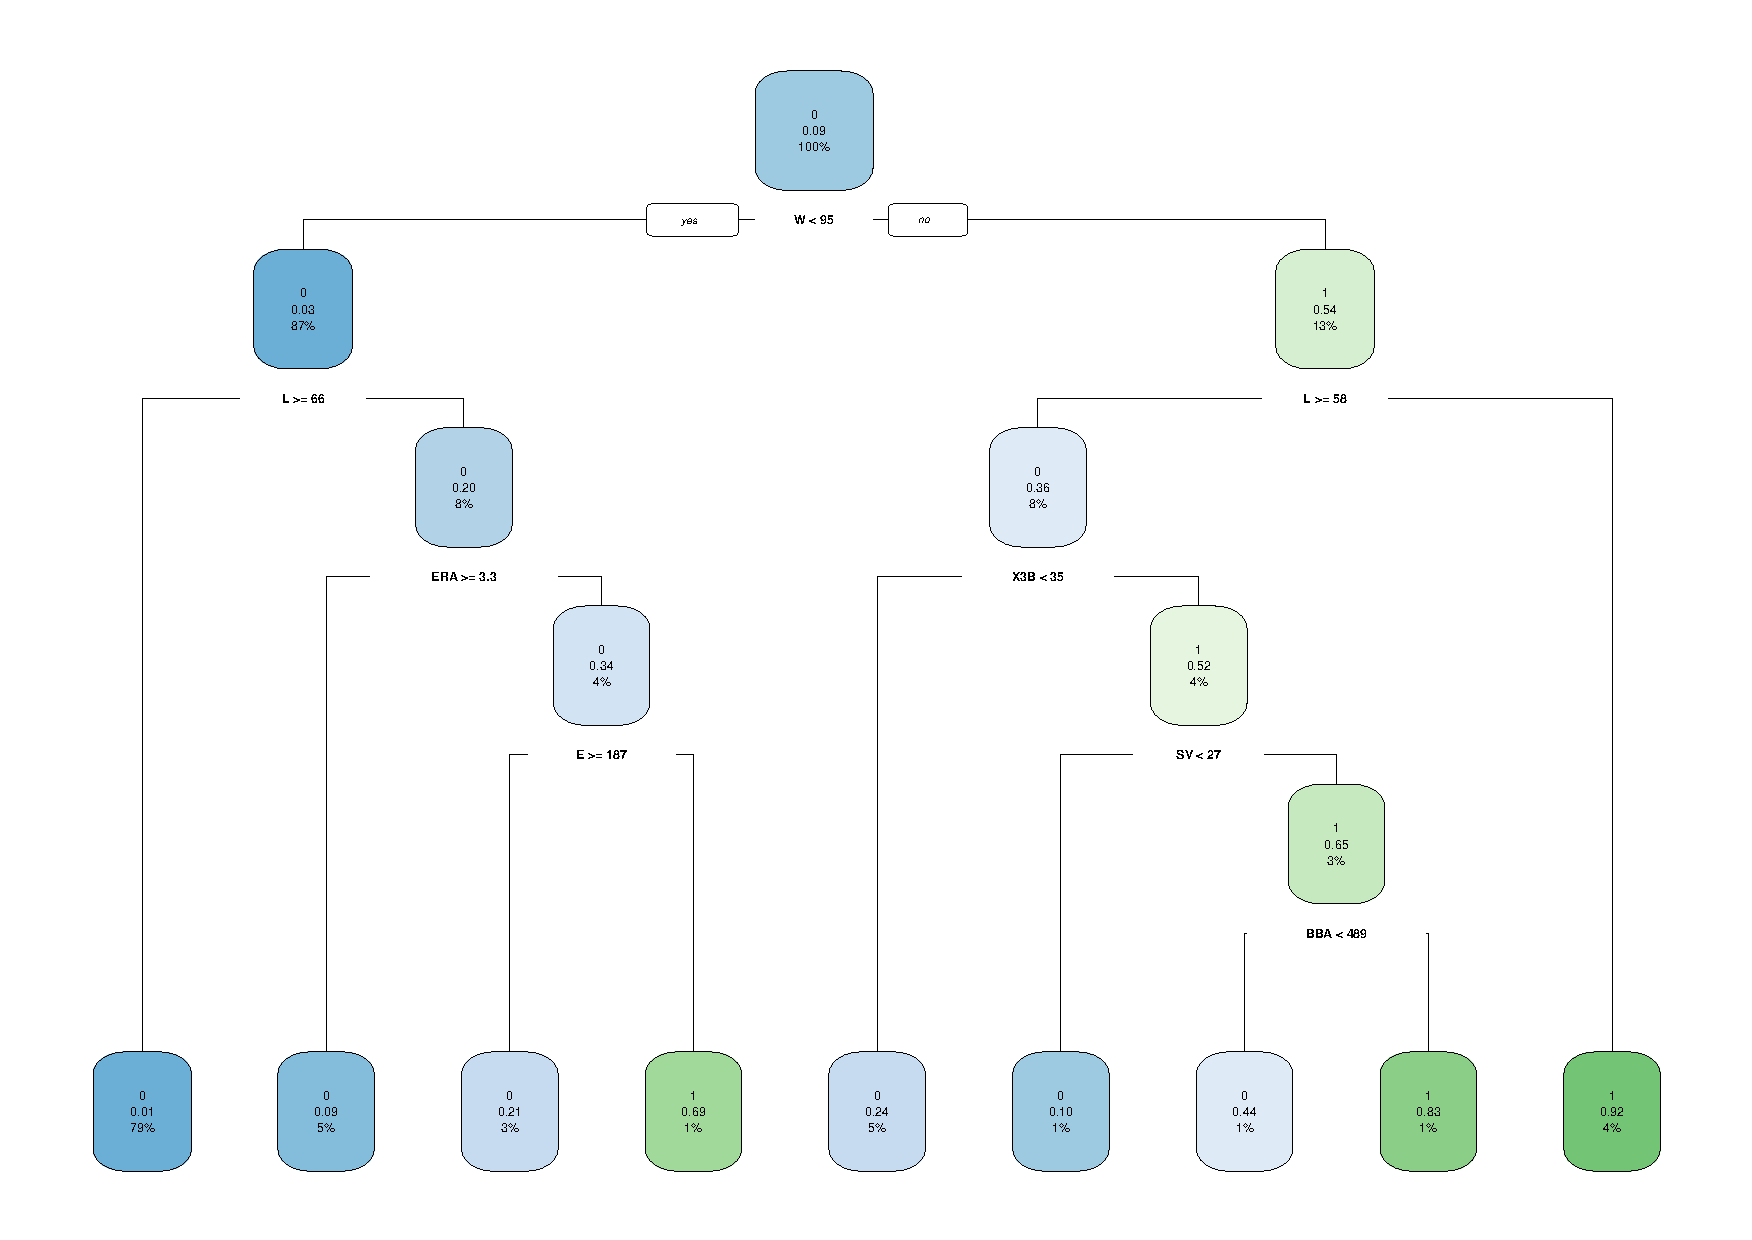
\includegraphics[width=10cm]{finalplots/classtree.pdf}
    \caption{CART Decision Tree for Playoff Prediction}
    \label{fig:classdt}
\end{figure}
We can now make a prediction using NL data resulting in the following accuracy tables and ROC curve:
\begin{minted}[frame=single]{R}
nlwinpred
       0    1
  0 1312   34
  1   97   46

[1] "Accuracy for test 0.912021490933512"
\end{minted}

\subsubsection{Comparing Gini to Information Gain}
By \cite{murthy1995}, one should expect both to perform equally.
We now test out this theory

\subsubsection{Changing Tree Size}
The first thing one can do to try and improve the Decision Tree is to adjust the parameters growing the tree which can change the size of the tree.
We obtain the following ROC Curves (Fig \ref{fig:rocall}) which have been compiled into one chart for comparison purposes.
\begin{figure}
    \centering
    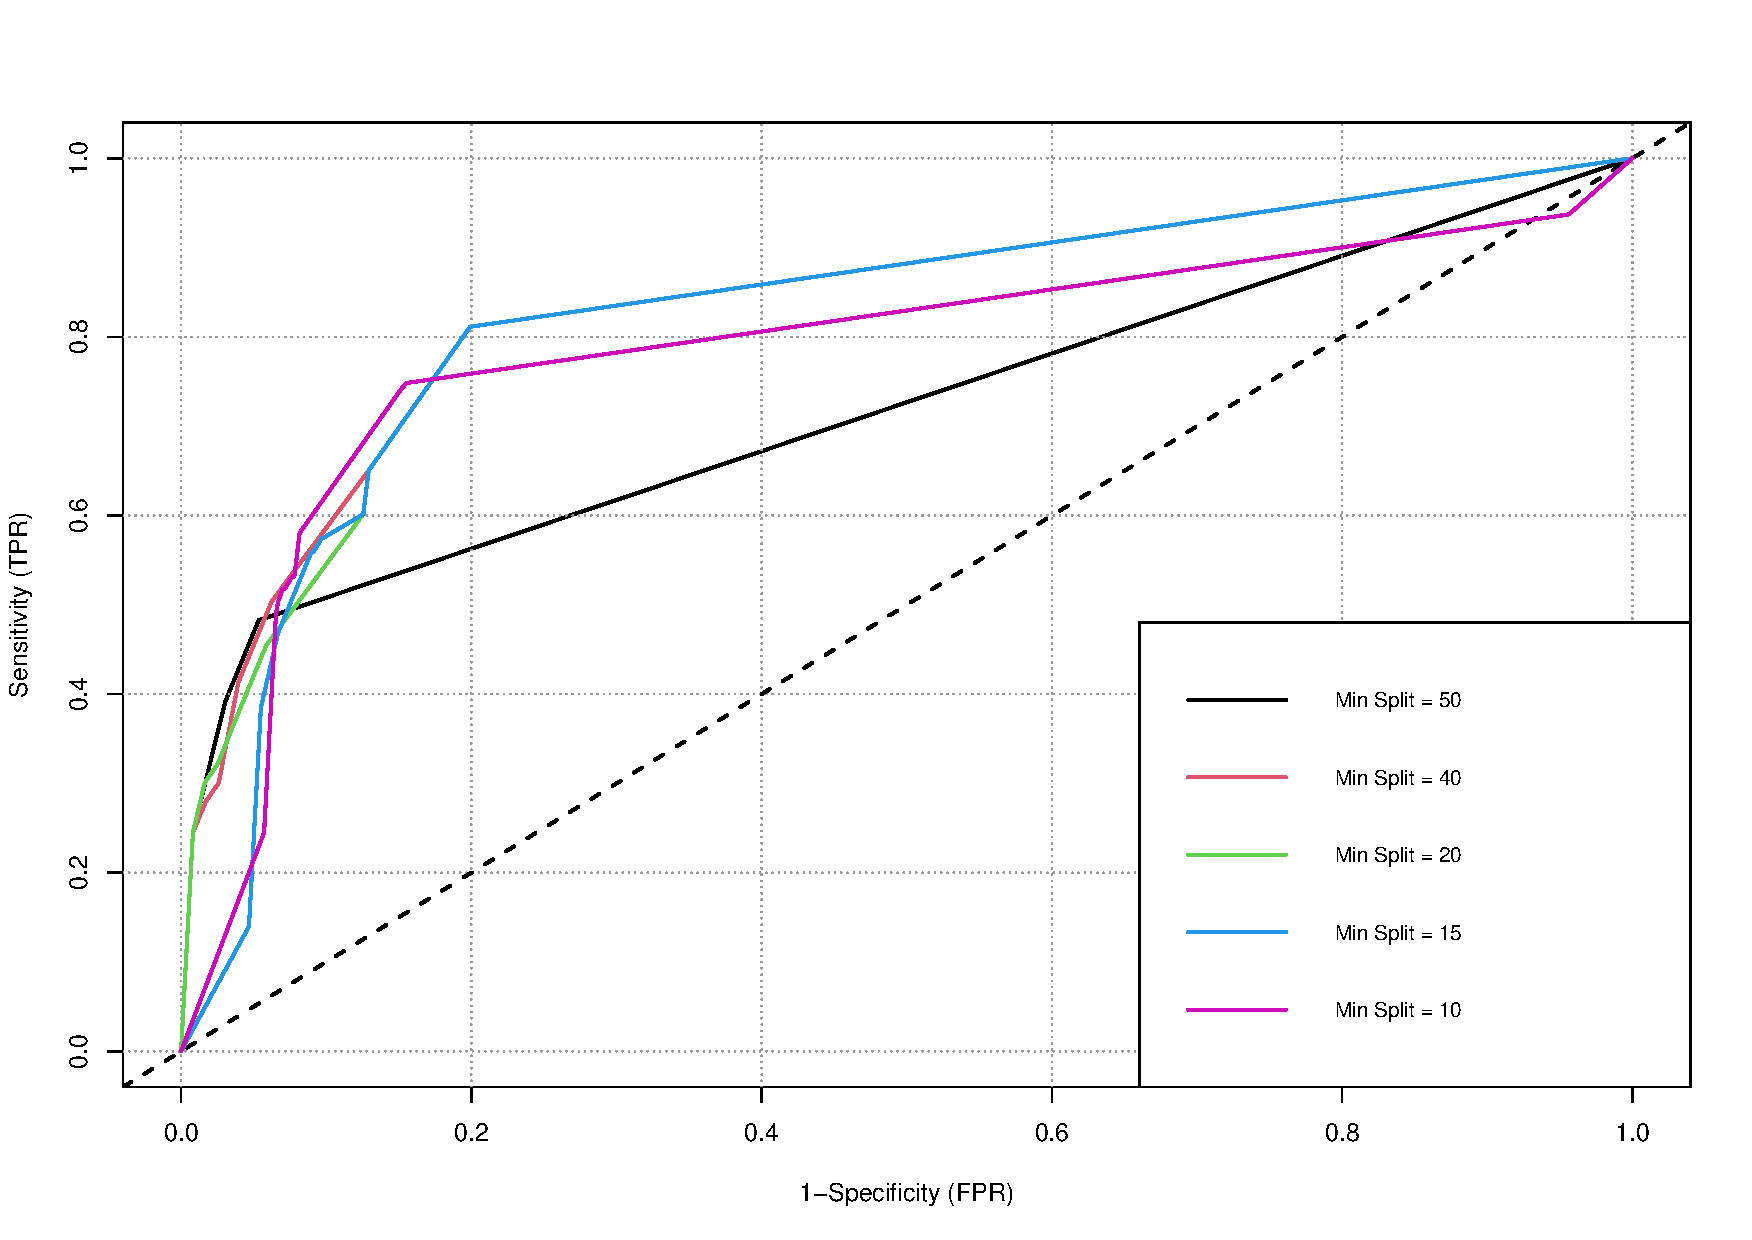
\includegraphics[width = 10cm]{reportcharts/roccurveall.pdf}
    \caption{ROC Curves for different sized Decision Trees}
    \label{fig:rocall}
\end{figure}\\
One can see (Table \ref{tab:allaucresults}) how over-fitting a model (as seen when \texttt{minsplit = 10}), that actually, you can make the tree perform worse as one can see with the following AUC results.
\begin{table}
    \centering
    \begin{tabular}{|c|c|c|}
        \hline
        \textbf{Minimum Split} & \textbf{Accuracy} & \textbf{AUC} \\
        \hline
        50 & 0.914036265950302 & 0.719765375783206 \\
        \hline
        40 & 0.909335124244459 & 0.836137116969212 \\
        \hline
        20 & 0.912021490933512 & 0.832934153513648 \\
        \hline
        15 & 0.888515782404298 & 0.821764045761074 \\
        \hline
        10 & 0.890530557421088 & 0.784855931586987 \\
        \hline
    \end{tabular}
    \caption{Table Showing Performance of Different Sized Tree Models}
    \label{tab:allaucresults}
\end{table}\\
This is because the tree is very biased in this scenario and therefore one would select a smaller tree which is more flexible in this scenario.
One notices that the accuracy of these models are very similar at around $\approx 90\%$, (likely due to the nature of the model being predicted) and thus in this case, the AUC is a much better predictor of model accuracy.

\subsubsection{Pruning}
Pruning simplifies complicated trees. 
Here we will show a small example of how it works. 
In reality, we would only start using pruning with much larger data sets and Decision Trees (Tree depth 20+ would often be needed to achieve a better result with pruning than growing a small tree and using Minimum Split as the stopping criterion).
\begin{table}
    \centering
    \begin{tabular}{|c|c|}
        \hline
        \textbf{Accuracy} & \textbf{AUC} \\
        \hline
        0.920080591000672 & 0.71908737621962 \\
        \hline
    \end{tabular}
    \caption{Results from Pruned Tree}
    \label{tab:prunescore}
\end{table}
\medskip\\
One notices that while the accuracy score remains similar (or in our case improves) the AUC score decreased as fewer nodes leads to fewer probabilities for ROC curves to be mapped onto.
In this scenario, while pruning simplifies the tree down a lot, as the AUC score is low and we really want to get accurate predictions of 1's, one would rather just use the full model in prediction.


\subsection{Additive Models - Bagging/Boosting}
We now try to see if the ``black box" methods in Chapter 4 provide improvements in accuracy of predictions to the model.
By nature of these models, we lost the interpretability of the model, but hope to gain accuracy compared to a regular Decision Tree.
We will be using Bagging, Random Forests, AdaBoost and xgBoost and comparing it with CART as we have seen previously.

\subsubsection{Comparison of Models}
\begin{table}
    \centering
    \begin{tabular}{|c|c|c|c|}
        \hline
        \textbf{Method} & \textbf{Implementation} & \textbf{Accuracy} & \textbf{AUC} \\
        \hline
        CART & {\color{blue} \texttt{rpart}} & 0.9120214909335 & 0.8329341535136 \\
        \hline
        Bagging & {\color{blue} \texttt{ipred}} & 0.9106783075890 & 0.9225080268914 \\
        \hline
        RF Bagging & {\color{blue} \texttt{randomForest(mtry=38)}} & 0.9106783075890 & 0.923666600858 \\
        \hline
        Random Forest & {\color{blue} \texttt{randomForest}} & 0.9153794492948 & 0.9199363044088 \\
        \hline
        AdaBoost & {\color{blue} \texttt{adabag}} & 0.9066487575554 & 0.9155955485822 \\
        \hline
        xgBoost & {\color{blue} \texttt{xgbTree}} & 0.9180658159839 & 0.9265682311745 \\
        \hline
        xgBoost & {\color{blue} \texttt{xgboost}} & 0.9126930826058 & 0.9272540238364 \\
        \hline
    \end{tabular}
    \caption{Table Showing how well Different Models Perform Relative to Decision Trees}
    \label{tab:allmodel}
\end{table}
Here, our data is quite bias so one obviously expects additive models to perform better than regular models. 
However, an interesting aspect is how Bagging and Random Forests perform comparatively well to the Boosting methods which is surprising since this suggests that the data has an equally high variance to go with the high bias.

\subsection{Using Optimizing Methods}
Using the above scores from Tables \ref{tab:octbag} and \ref{tab:octauc}, one can see the following scores,
\begin{table}
    \centering
    \begin{tabular}{|c|c|c|}
        \hline
        \textbf{Model} & \textbf{Accuracy} & \textbf{AUC}  \\
        \hline
        CART & 0.9120215 & 0.8329341535136 \\
        \hline
        Pruning & 0.9200806 & 0.719087376220 \\
        \hline
        OCT & 0.9140363 & 0.7018256631927 \\
        \hline
        Gini OCT & 0.8932169 & 0.8238525961409 \\
        \hline
        Bagged OCT & 0.9120215 & 0.9237860950342 \\
        \hline
    \end{tabular}
    \caption{Comparing CART to OCT}
    \label{tab:cartoctclass}
\end{table}
\begin{figure}
    \centering
    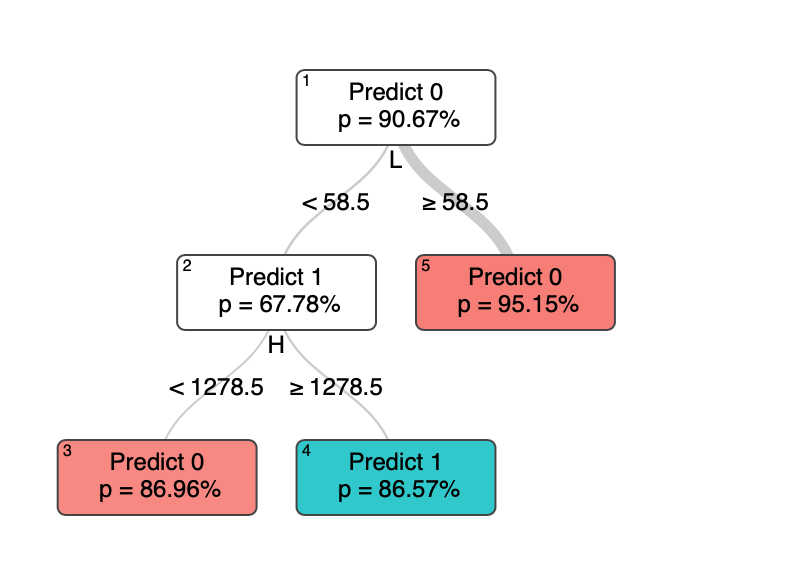
\includegraphics[width = 10cm]{reportcharts/oct1.png}
    \caption{OCT}
    \label{fig:octplayoff}
\end{figure}
One can see that OCT (Figure \ref{fig:octplayoff}) actually performs more similarly to the Pruned Tree than the regular tree in terms of AUC score, which is to be expected with such small trees we had.
This is a bit unexpected as one would expect a new method to perform better than the status quo but it is likely that the nature of the data and the small tree size has led to this poor output as Dunn had noted in \cite{oct}.
One expects playing around with the parameters would lead to some improvements to the model.
\medskip\\
One also notices that using Gini (see \cite{oct} and figure \ref{fig:ginioct}) as the criterion for labelling our incorrect predictions instead of just regular misclassification labelling improves our model.
This supports what we said earlier about how Gini is a much better metric for tree-based models than misclassification error.
\begin{figure}
    \centering
    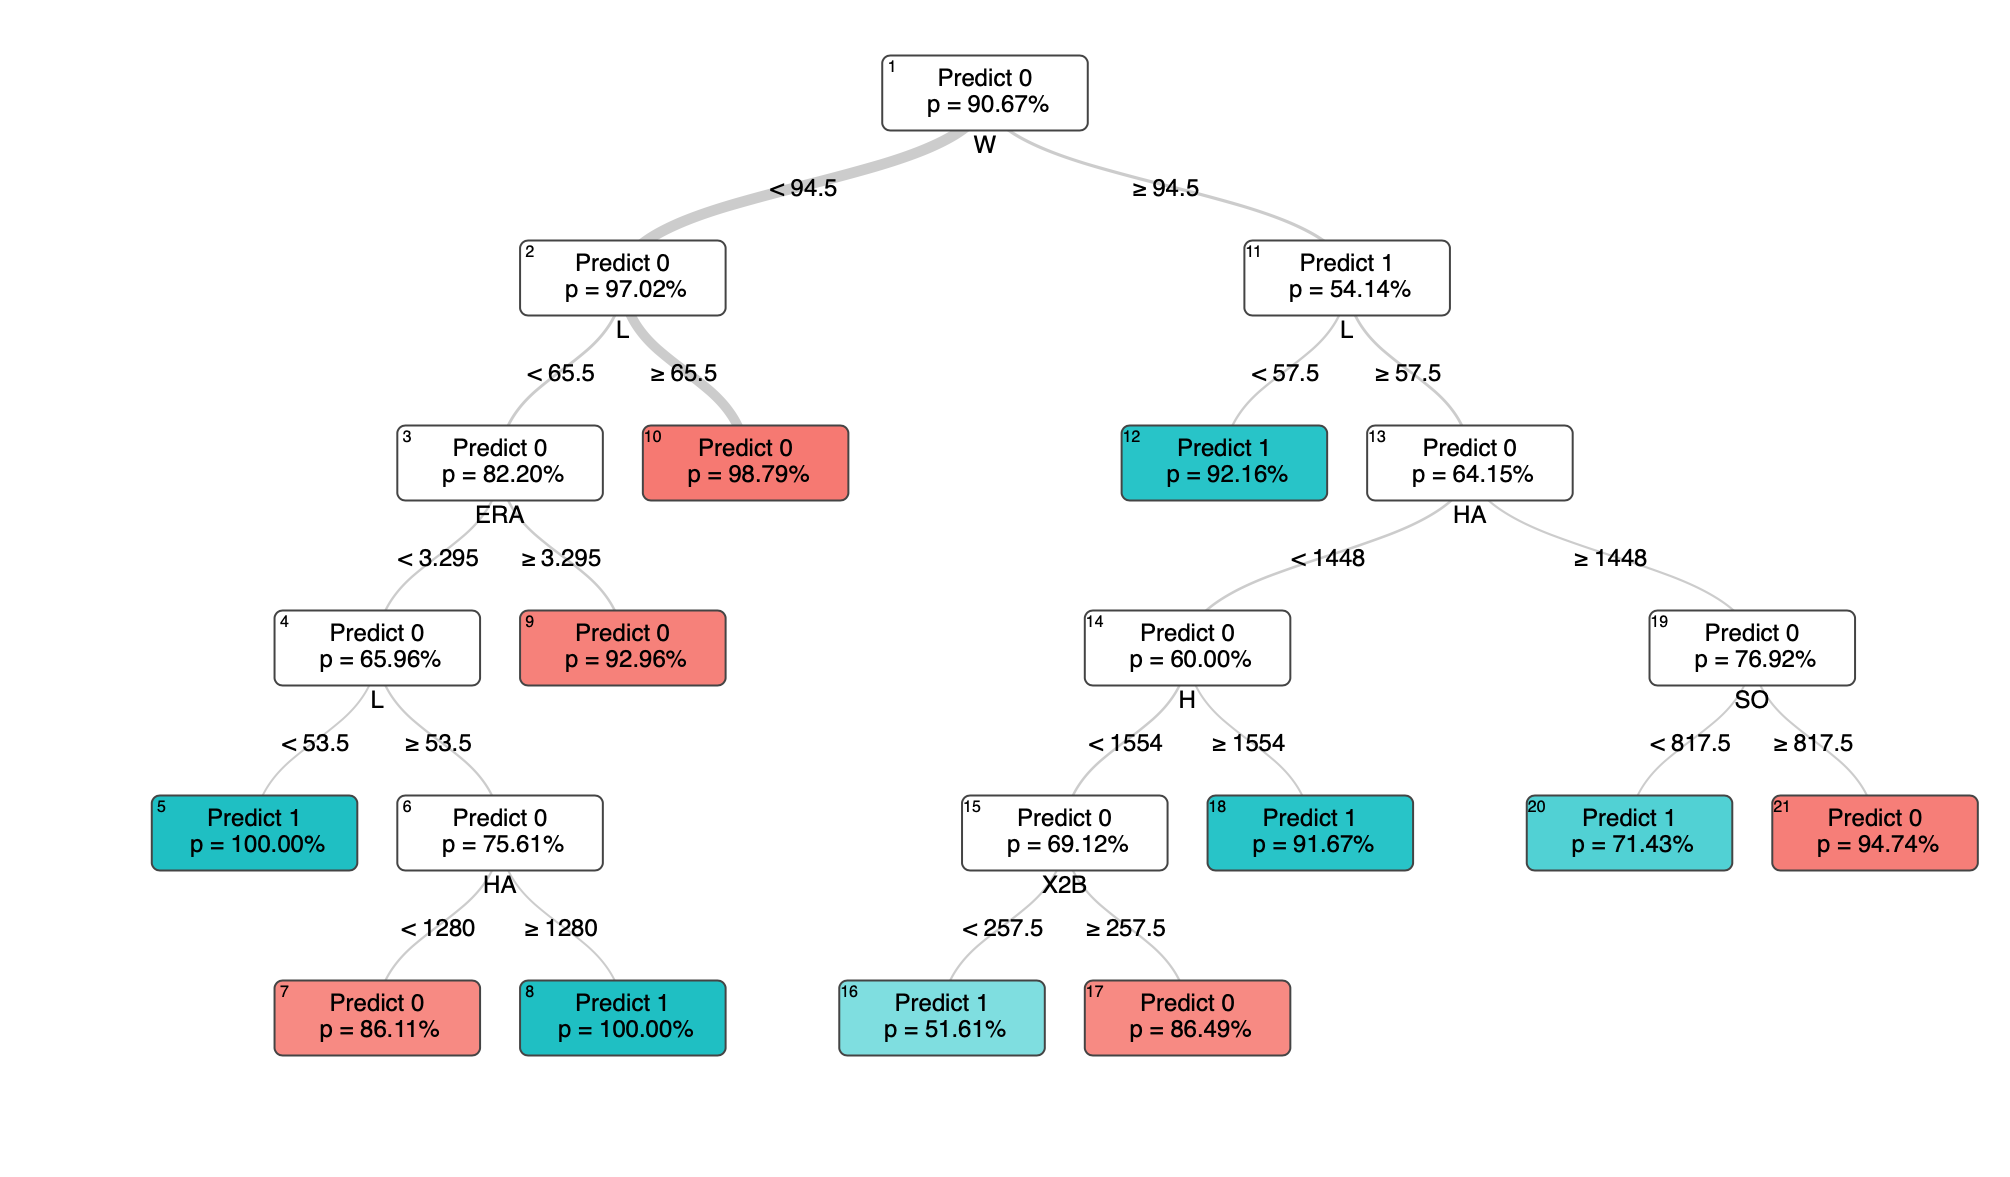
\includegraphics[width = 10cm]{reportcharts/ginioct.png}
    \caption{Gini OCT}
    \label{fig:ginioct}
\end{figure}
\begin{figure}
    \centering
    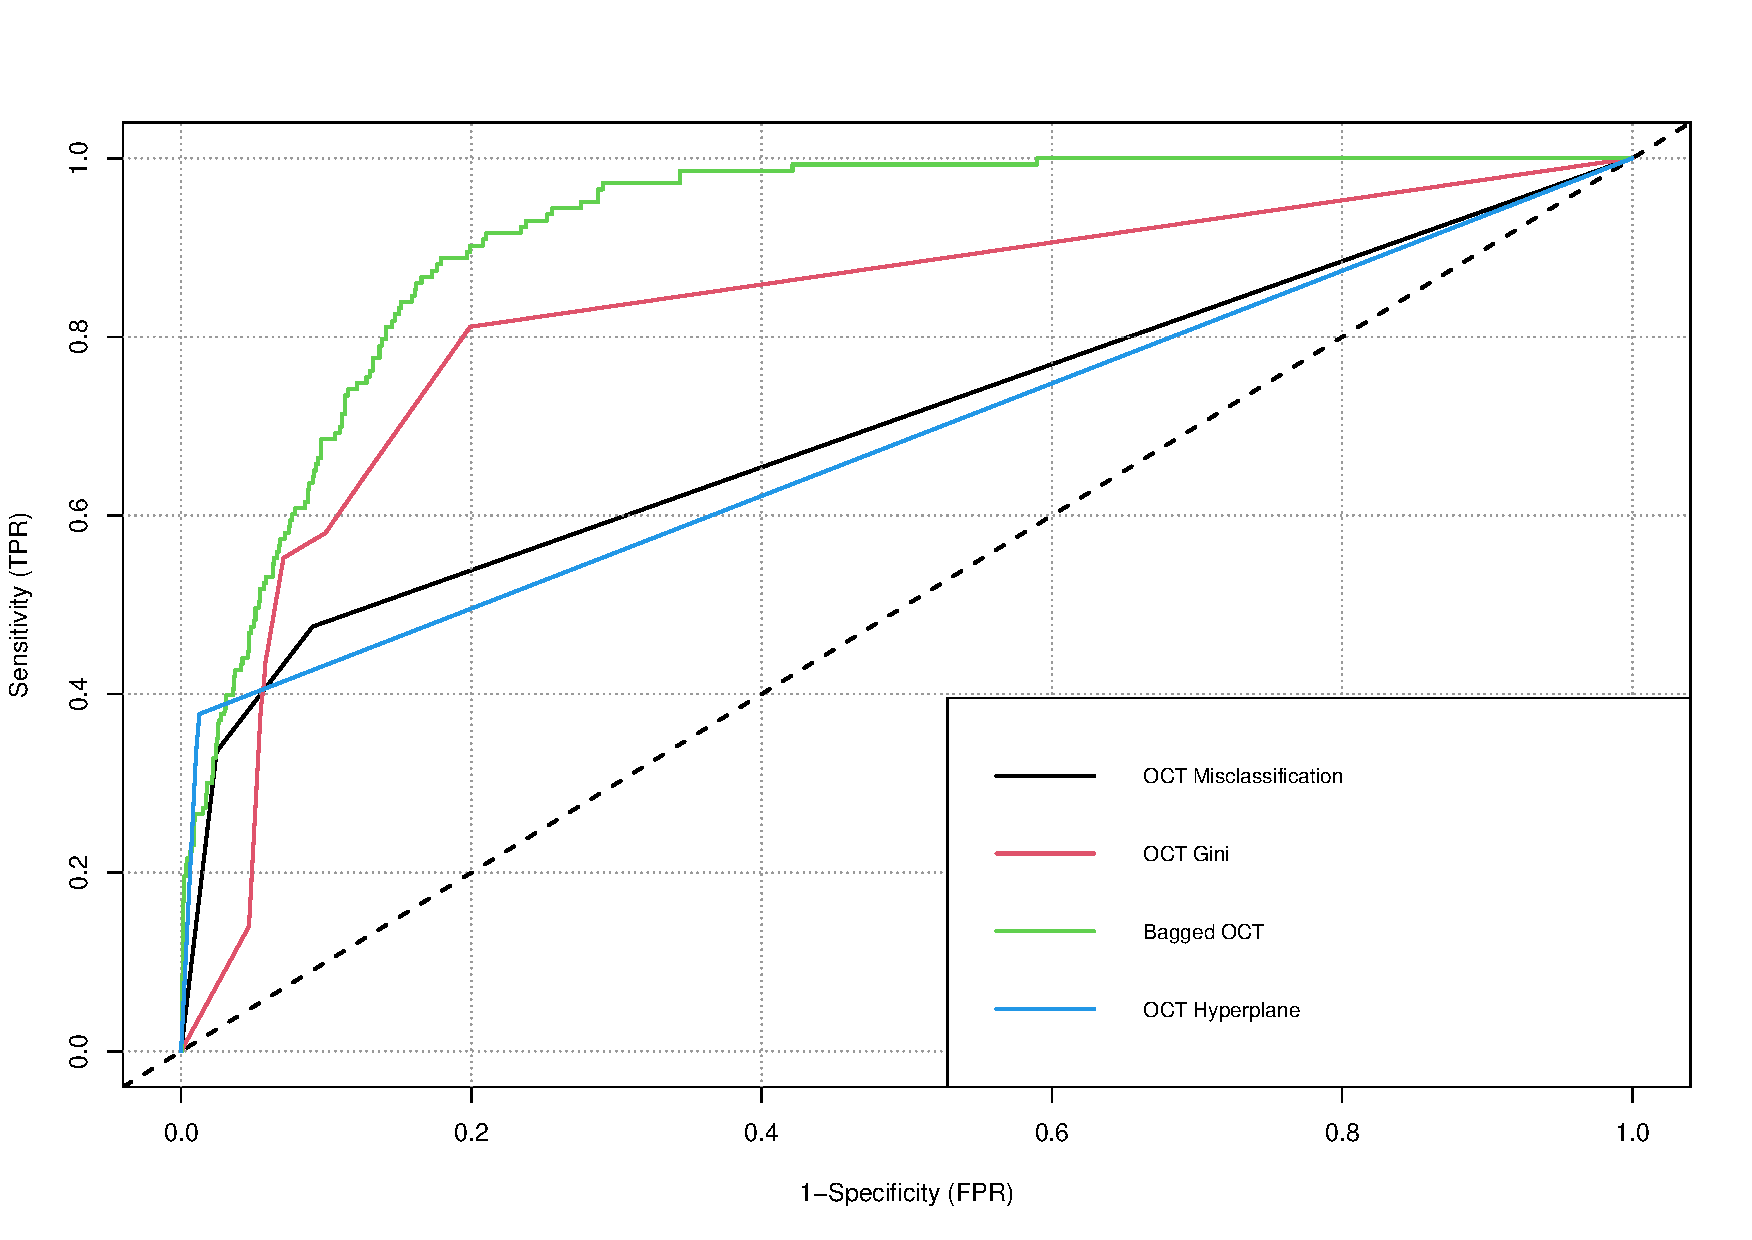
\includegraphics[width = 8cm]{reportcharts/alloctroc.pdf}
    \caption{ROC curves for all OCT models}
    \label{fig:allrococt}
\end{figure}




\section{Salary Prediction}
Similarly to above, one can also see the natural progression of Regression Trees from the base tree to something much more complex.
In this case, we will not go into as much detail as we did for classification, however, the code will be left in the Appendix for the reader to adjust if one were curious about how changing parameters would affect the model.
\medskip\\
In this case, we will be looking at player salaries for a given year and predicting how much value a player gave the team given their outputs.
This is useful for teams as a player's statistics do not vary as much each year and so a can predict salaries easily which is helpful for team construction. 

\subsection{Linear Regression}
Before we proceed, one should always check to see if linear regression is already a suitable model.
We find the following result provides the best linear fit.
\subsubsection{Linear Model}
After using step-wise methods to reduce the model from full size, one finds that our model can be fitted using,
\begin{minted}{R}
reglmstep <- lm(formula = salary/1e+06 ~ stint + G + H + X3B + HR + RBI  
                + BB + SO + IBB + SH, data = salarybatting)
\end{minted}
Which results in an RMSE score of $\$4,302,863$.
When plotting to check how well the model predicted against the actual salary however, we find that our model here performs very poorly as seen in Figure \ref{fig:lmmodel}.
\begin{figure}
    \centering
    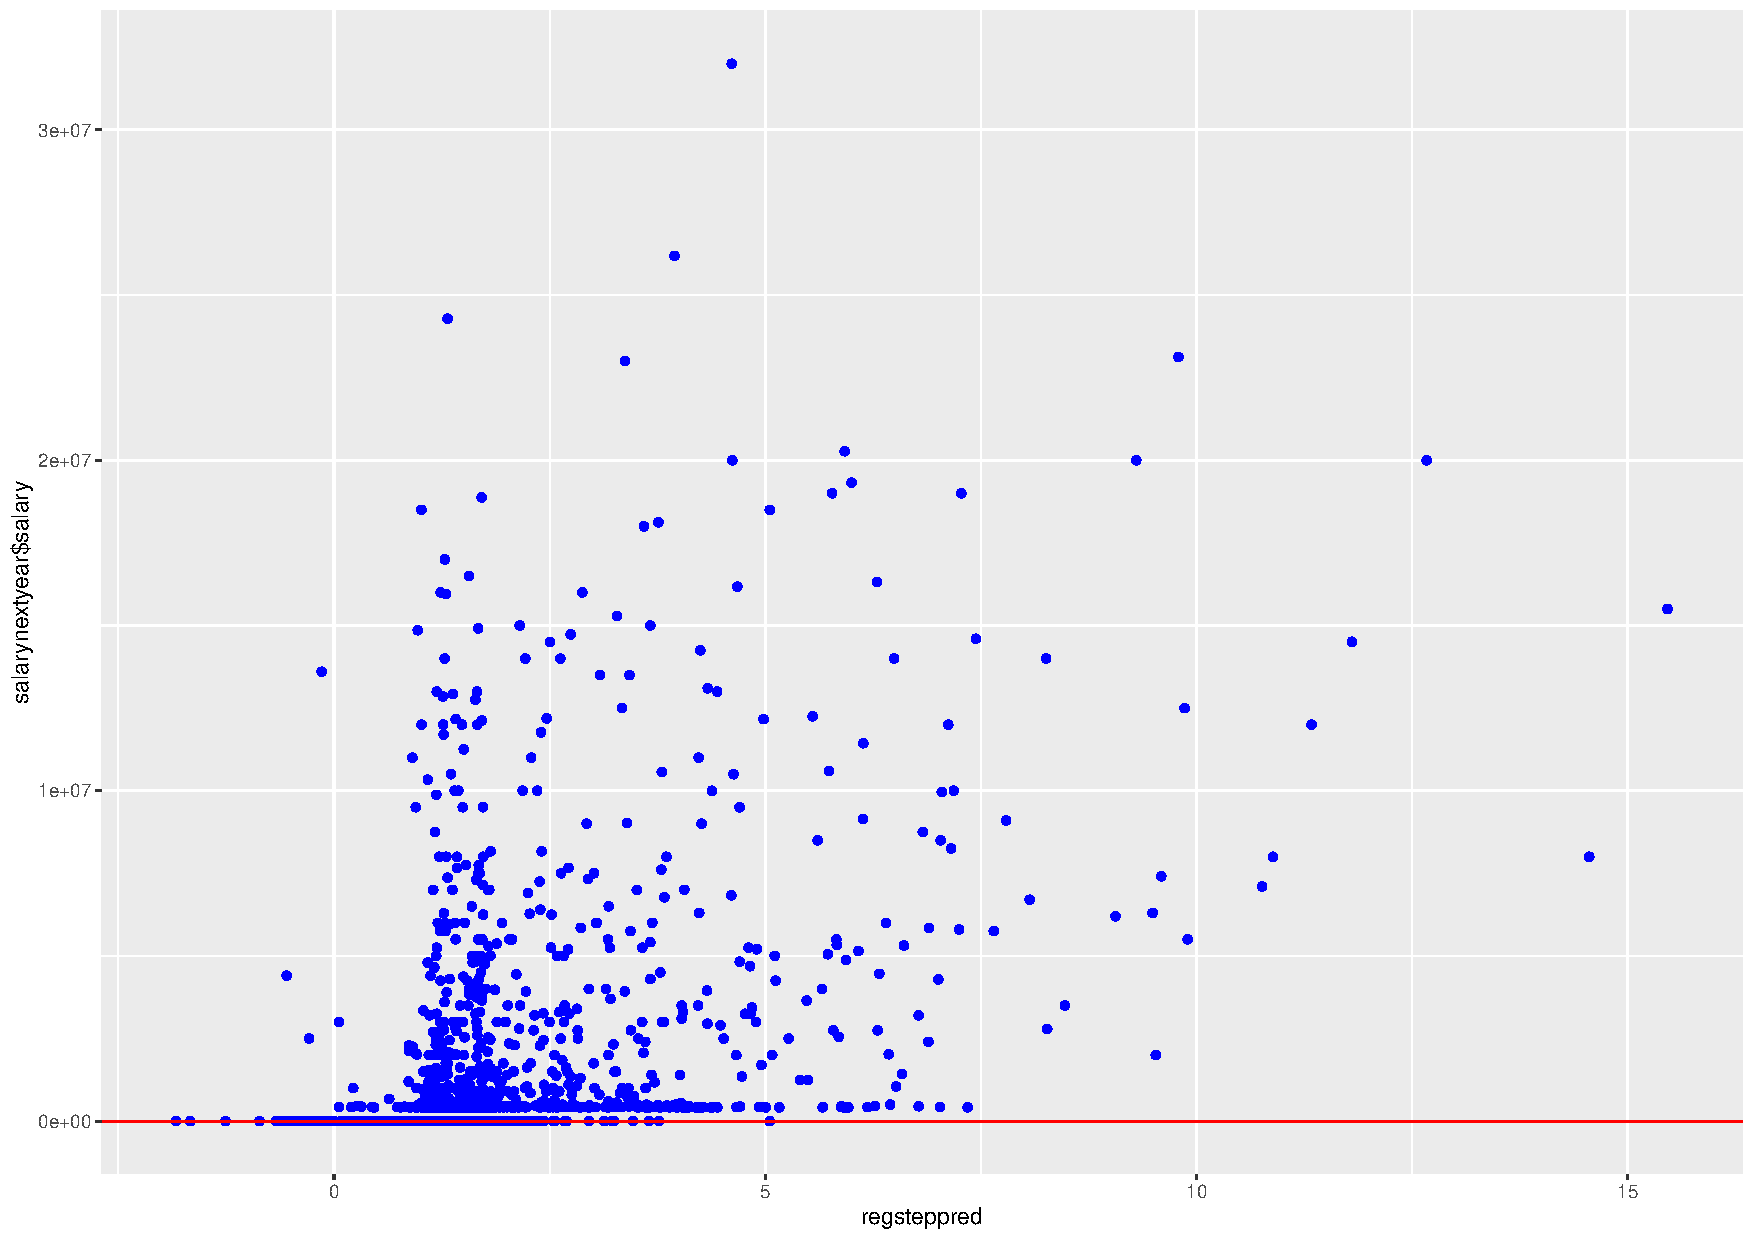
\includegraphics[width = 10cm]{reportcharts/salarylmcomp.pdf}
    \caption{Plot of Predicted vs Actual Salaries}
    \label{fig:lmmodel}
\end{figure}
This is in fact a very poor predictor and thus one can safely proceed onto Tree-Based methods in hopes of finding a better model.

\subsection{All ROC Curves}
Summing up all of the above, we can compare all these ROC together to see how each model compares with each other.
One can see that with our dataset, it may be better for us to sacrifice interpretability for accuracy if one wants the best predictive model.
However, using Gini as a criterion, one can create an interpretable model which sacrifices a bit on accuracy but is still good enough for us to use as a flexible basis. \begin{figure}[h]
    \centering
    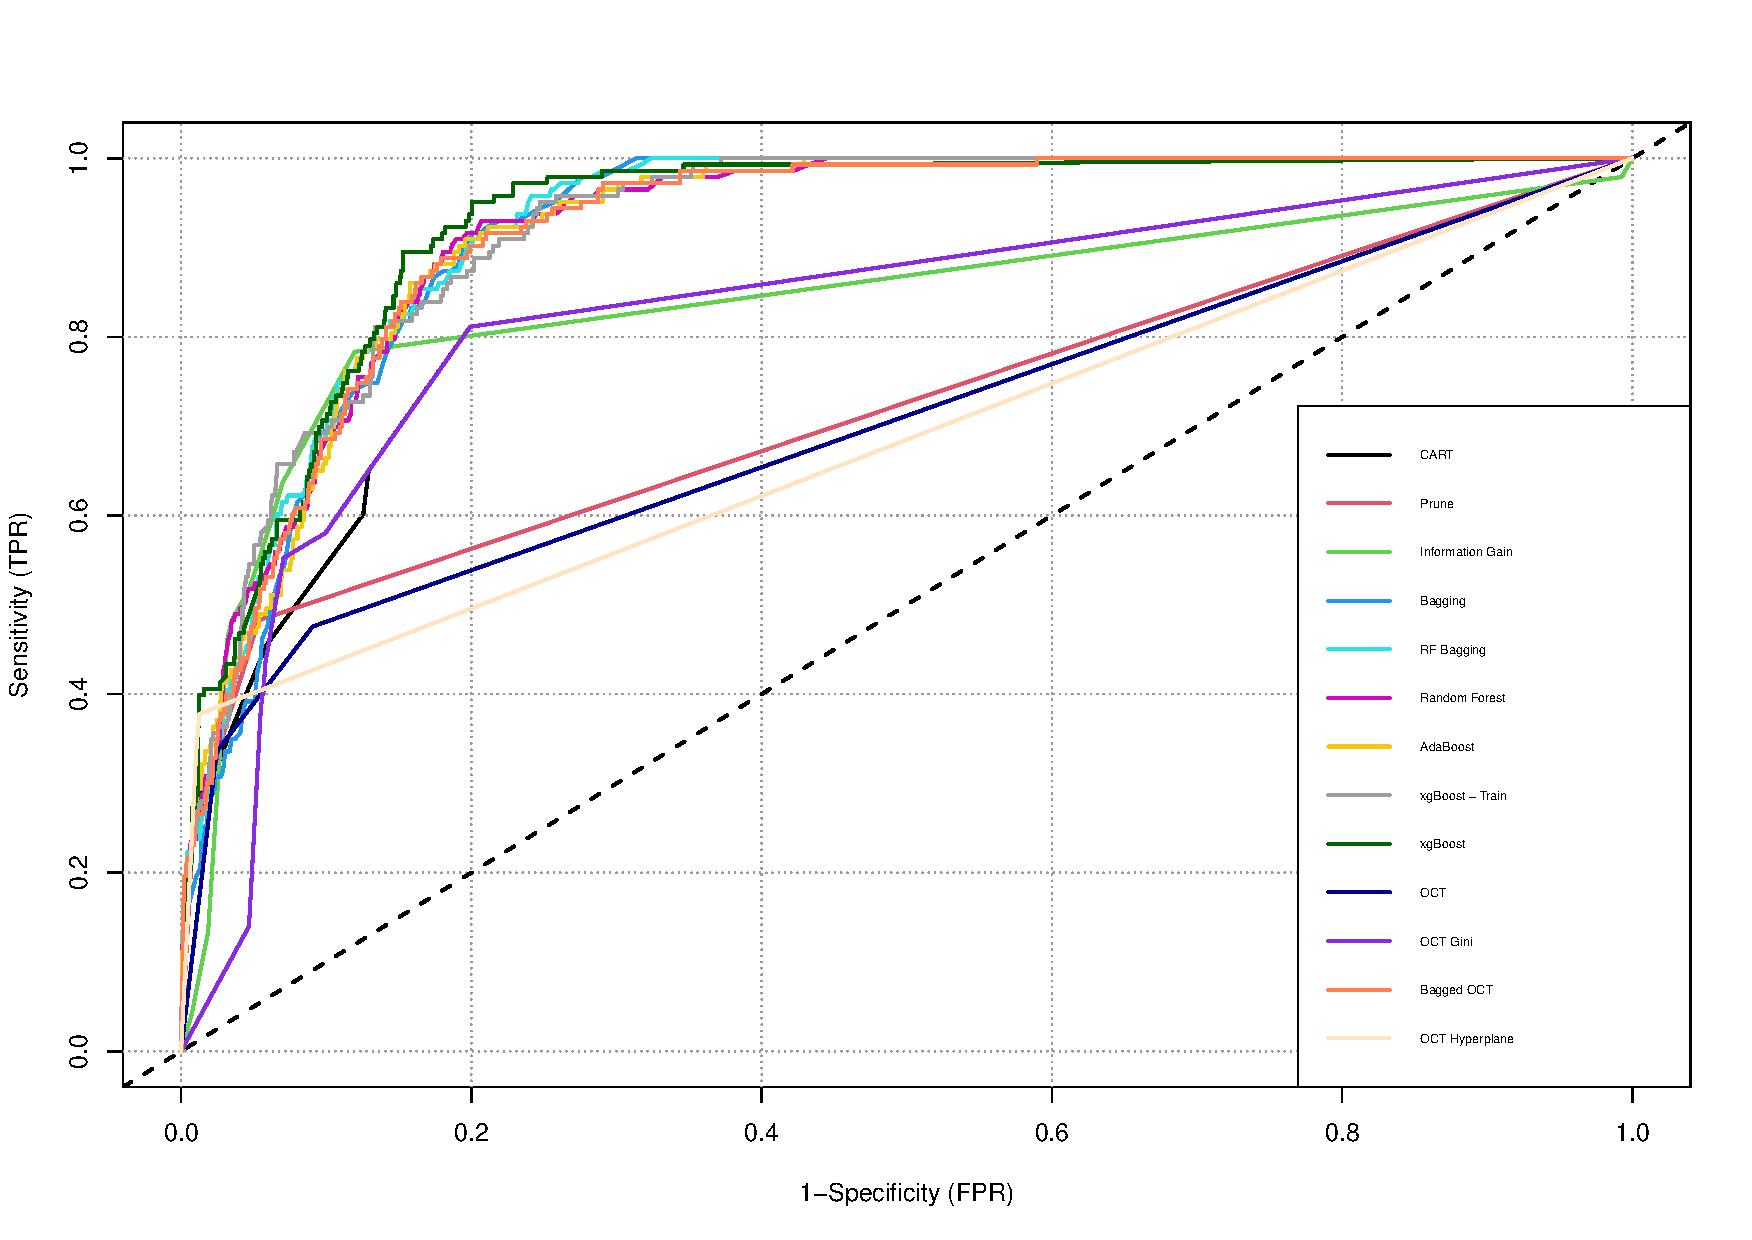
\includegraphics[width = 10cm]{reportcharts/ROC.pdf}
    \caption{Summary of all ROC curves}
    \label{fig:allroccurves}
\end{figure}

\subsection{Regression Tree}
\begin{center}
    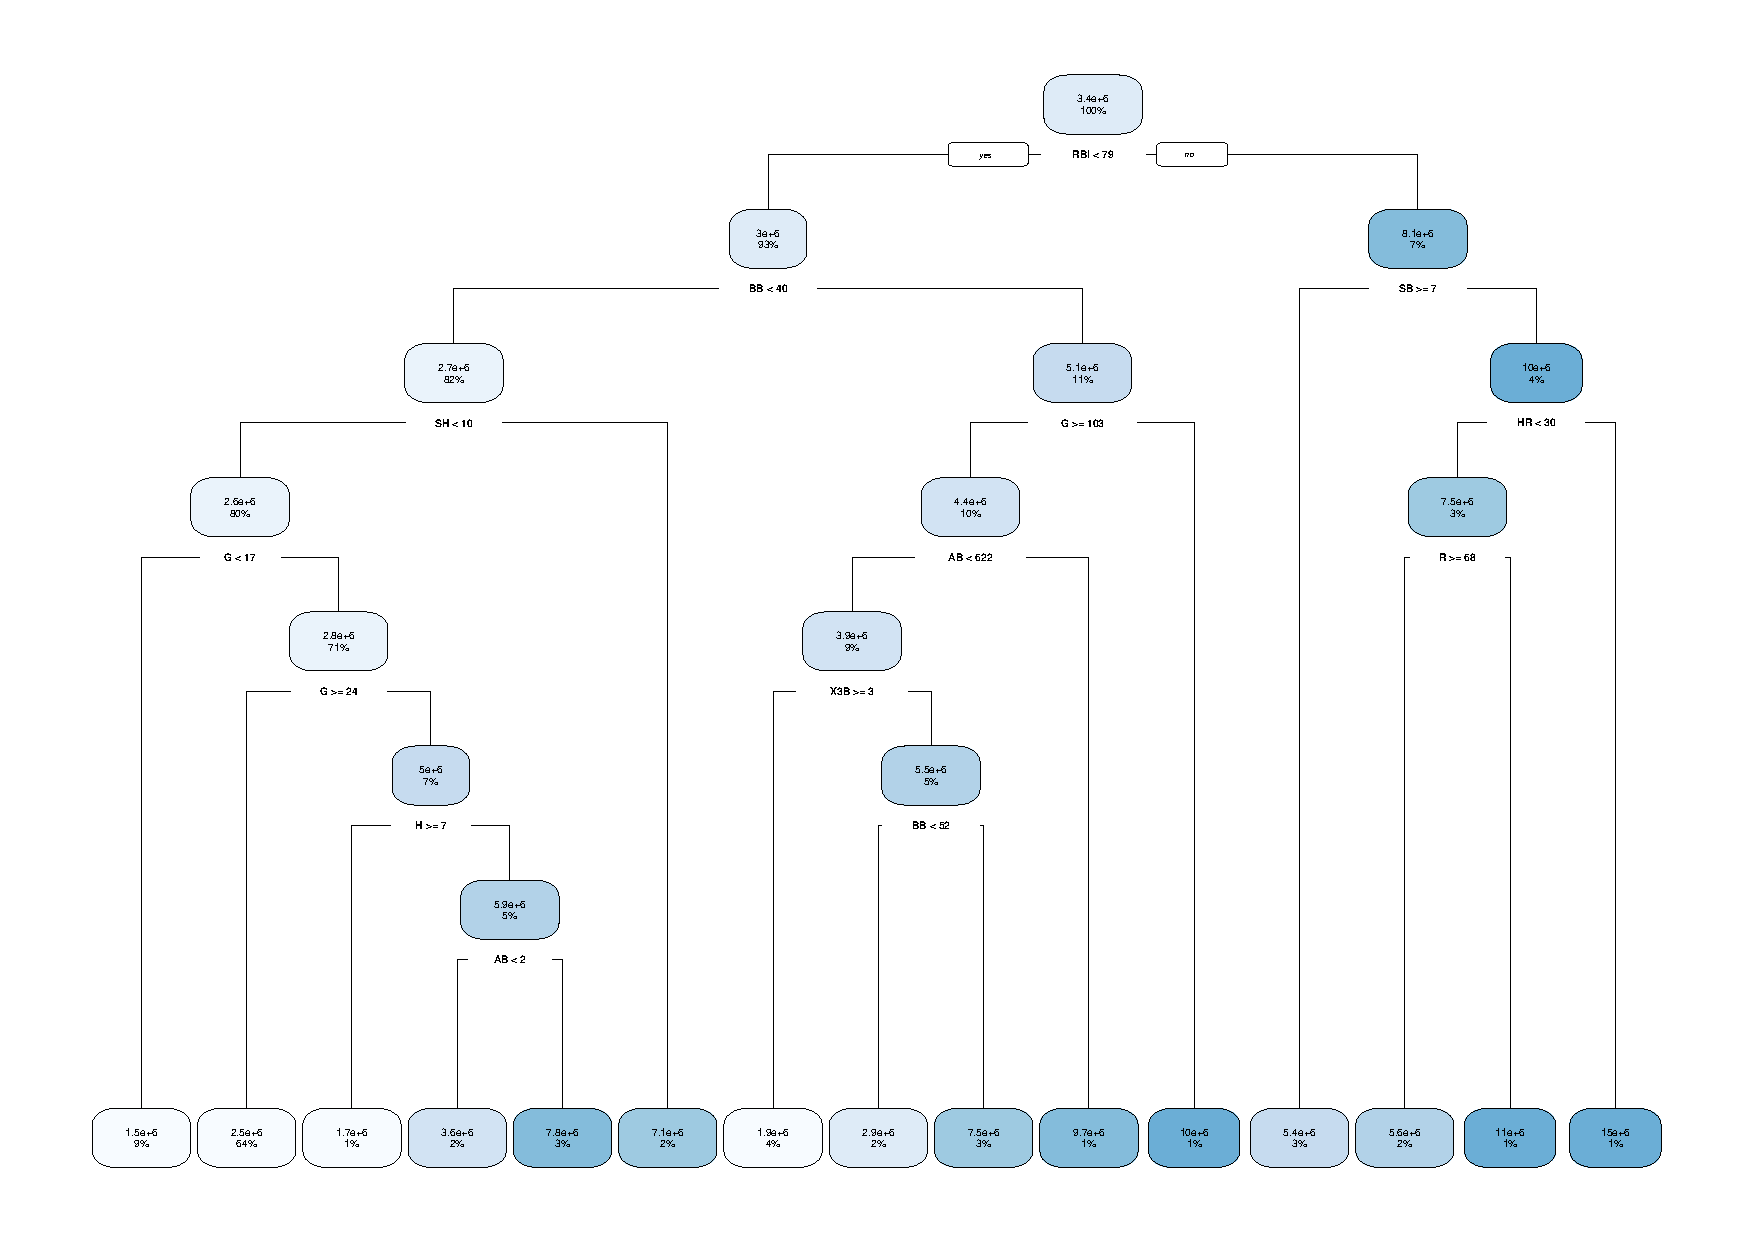
\includegraphics[width=0.7\linewidth]{finalplots/regtree.pdf}
    \label{fig:regtree}
\end{center}
Here we have a decision tree for baseball players salaries using data from the \texttt{Lahman} Dataset (Lahman) for the year 2010.
We note that the accuracy of this predictor can be found by calculating the Residual Mean Square Error (RMSE) value.
In this case we used data from the next year (2011) as a test dataset and achieved the following RSME scores (Table \ref{tab:regrsme})
\begin{table}
    \centering
    \begin{tabular}{|c|c|}
        \hline
        RMSE & \$3,479,857 \\
        \hline
    \end{tabular}
    \caption{RMSE score of Regression Tree}
    \label{tab:regrsme}
\end{table}

\subsection{Other Methods}
As we have done for classification, we are able to build multiple models using different techniques based off the same salary dataset.
We are able to use the exact same libraries as before and thus it seems trivial to extend our application to other tree based methods.
Table \ref{tab:allreg} provides us with a summary of all the Root Mean-Squared Error (RMSE) scores for all models for comparison.
\begin{table}
    \centering
    \begin{tabular}{|c|c|}
        \hline
        \textbf{Model} & \textbf{RMSE} \\
        \hline
        Linear Regression & \$4,302,863 \\
        \hline
        CART & \$3,479,857 \\
        \hline
        Pruned CART & \$3,492,685 \\
        \hline
        Bagging & \$3,298,992 \\
        \hline
        Random Forest & \$3,299,106 \\
        \hline
        xgBoost & \$3,386,000 \\ 
        \hline
        Optimal Regression Tree & \$3,561,030 \\
        \hline
        ORT Hyperplane & \$3,561,030 \\
        \hline
    \end{tabular}
    \caption{Table showing RMSE scores of all models in our regression example for salary}
    \label{tab:allreg}
\end{table}
\medskip\\
The first thing one notices is how well CART already performs by itself without adding anything on top of it.
We also see that the variance reducing methods of Bagging and Random Forests provide the best improvement to the model.
As salaries are highly variable, this is to be expected, although its key to note that the improvement is not that great when compared with the improvement one gets from just moving from linear regression to tree methods.
\medskip\\
An interesting factor is that the modern Optimal Regression Tree Methods (Figure \ref{fig:ort} and \ref{fig:orth}) did not perform better than even the Pruned CART approach which is not expected as the method of construction of this method should be leading to both having much more similar RMSE scores. One supposes that using the quadratic loss for each predictor may have been a factor as that would penalize the variance in the data set more than you would using CART as the error there is more localized in the regions one gets.
\begin{figure}
    \centering
    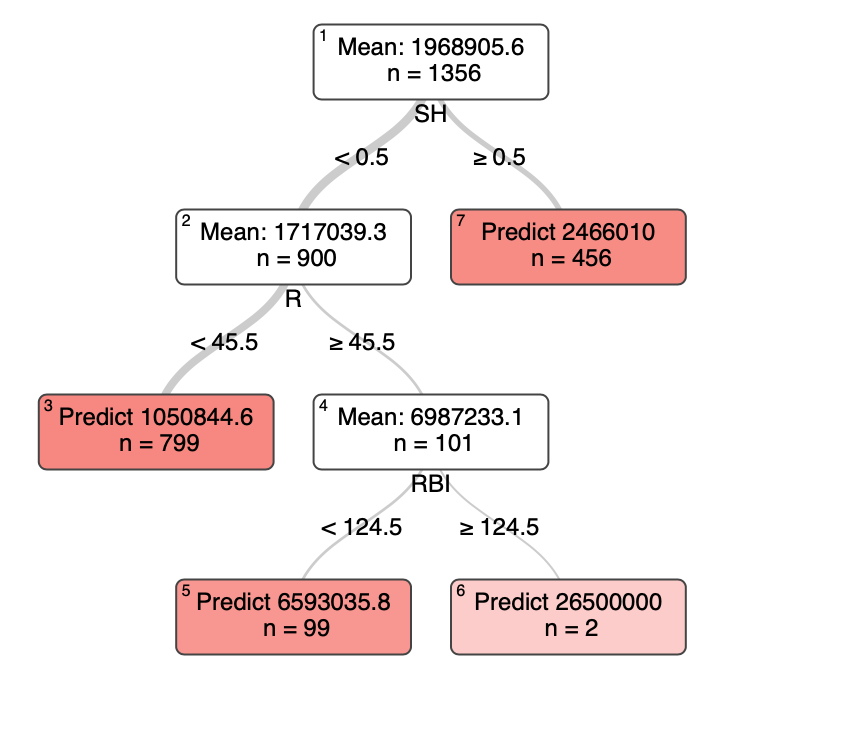
\includegraphics[width = 8cm]{reportcharts/ort.png}
    \caption{Optimal Regression Tree}
    \label{fig:ort}
\end{figure}
\begin{figure}
    \centering
    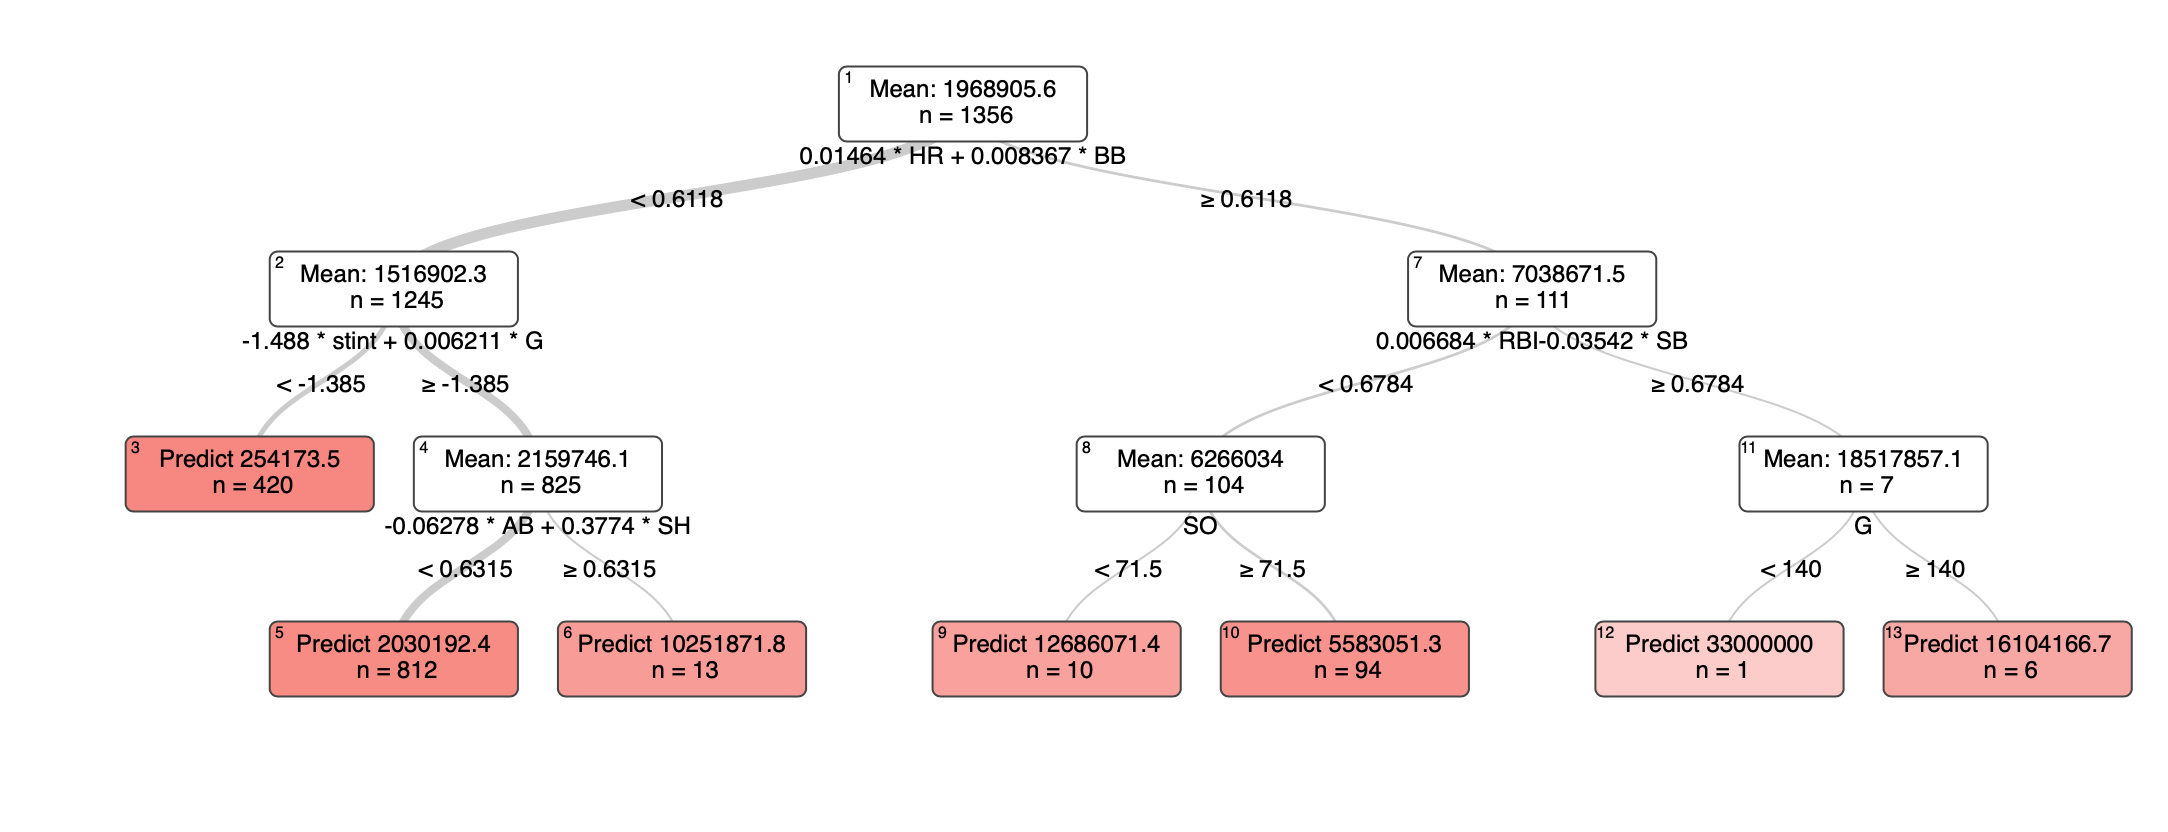
\includegraphics[width = 12cm]{reportcharts/orth.png}
    \caption{Optimal Regression Tree with Hyperplane}
    \label{fig:orth}
\end{figure}


\chapter{Conclusion}
One can see that Tree-Based Methods are a very strong Supervised Statistical Machine Learning Method. 
They are very robust and predict reasonably well.
They are also one of the best base learning methods as we can use trees as a base for all the methods we have seen today.
\medskip\\
We have also observed that the interpretability of models, while useful in many cases, often lend to loss of accuracy as they tend to not be as flexible on the overall predictor. 
While they still maintain their place in modern Machine Learning, it may be better for one to avoid using it unless you have a specific visual reason to use it.
Another note is that the modern Optimal Tree method which was built as an attempt to optimize trees using Mixed-Integer Programming methods still do not outperform the more traditional ``blackbox" methods that we have today, however, the potential is there and some minor changes to flexibility with regards to high bias and high variance models may be needed before more typical use.
\medskip\\
On that note, the use of a high-bias and a high-variance sample was useful to show how these models behave in more real world scenarios where the data is ``not nice" and thus it is very hard to predict using basic methods such as linear regression, for example. 
\bigskip\\
Applying the methods we have seen in practical terms as we have done in the previous chapter, we can now use one of the models that we have fitted and apply it to new unseen data.
This is what happens in the real world with propensity models in more than just baseball.
In terms of baseball this is a great way to show how teams decide on where a team needs to improve to increase their chances of being successful and then onto how much a team should spend to achieve these goals they have set for themselves.
In real life, much more depth is involved and many more models and methods would be used but this is already a great start in terms of how teams actually operate.




\chapter*{Acknowledgments}
\addcontentsline{toc}{chapter}{Acknowledgments}
\pagenumbering{roman}
Firstly, I would like to that my supervisors Professor Peter Craig and Dr Louis Aslett for help and guidance with this project, without whom, I would not be writing this project.
\bigskip\\
I would also like to thank Daisy Zhuo and the rest of the Interpretable AI \texttt{IAI} team for providing me access to the software needed for me to be able to try out the new method that we will be implementing in this project \textbf{The Optimal Classification/Regression Tree}.\\
{\color{violet}Due to the computationally taxing nature of MIO's, it is not easy for one to do this at home.
If one were to wish to do so by hand, a good place to start is to use {\color{blue} \texttt{Gurobi}} or other programming optimization software as a place to start.
\medskip\\
In this case, I was able to run an {\color{blue} \texttt{R}} interface of the {\color{blue} \texttt{Julia}} programme.
With this I would like to thank Daisy Zhuo at Interpretable for giving me access to the IAI package.}


\bibliographystyle{apalike}
\bibliography{reference}

\begin{appendices}
\chapter{Extracting Training and Testing Datasets}
We have selected four sets of data to work on this project, one each for classification and regression. Below is the code for the data and the variables we have selected in each.

\subsubsection{Playoff - Classification}
The following is to predict whether a team would win the league given how well a team did throughout the season. Here is the code to isolate the data:
\subsubsection{Training Data}
\begin{minted}[frame = single]{R}
teamseason <- Lahman::Teams
head(teamseason)
alplayoff <- filter(teamseason, teamseason$lgID =="AL")
head(alplayoff)
is.factor(alplayoff)
alplayoff[alplayoff =="N"] = 0
alplayoff[alplayoff =="Y"] = 1
head(alplayoff)
alplayoff %>% filter(!is.na(LgWin))
alplayoff1 = subset(alplayoff, 
                    select = -c(Rank, park, WSWin, 
                                name, teamID, franchID, teamIDBR,
                                teamIDlahman45, teamIDretro))
alplayoff1$LgWin <- as.factor(alplayoff1$LgWin)
alplayoff1[is.na(alplayoff1)] <- 0
\end{minted}





\subsubsection{Testing Data}
\begin{minted}[frame = single]{R}
nlplayoff <- filter(teamseason, teamseason$lgID =="NL")
head(nlplayoff)
is.factor(nlplayoff)
nlplayoff[nlplayoff =="N"] = 0
nlplayoff[nlplayoff =="Y"] = 1
head(nlplayoff)
nlplayoff %>% filter(!is.na(LgWin))
nlplayoff1 = subset(nlplayoff,
                    select = -c(Rank, park, WSWin, 
                                name, teamID, franchID, teamIDBR,
                                teamIDlahman45, teamIDretro))
nlplayoff1$LgWin <- as.factor(nlplayoff1$LgWin)
nlplayoff1[is.na(nlplayoff1)] <- 0
\end{minted}



\subsubsection{Salary - Regression}
\begin{figure}
    \centering
    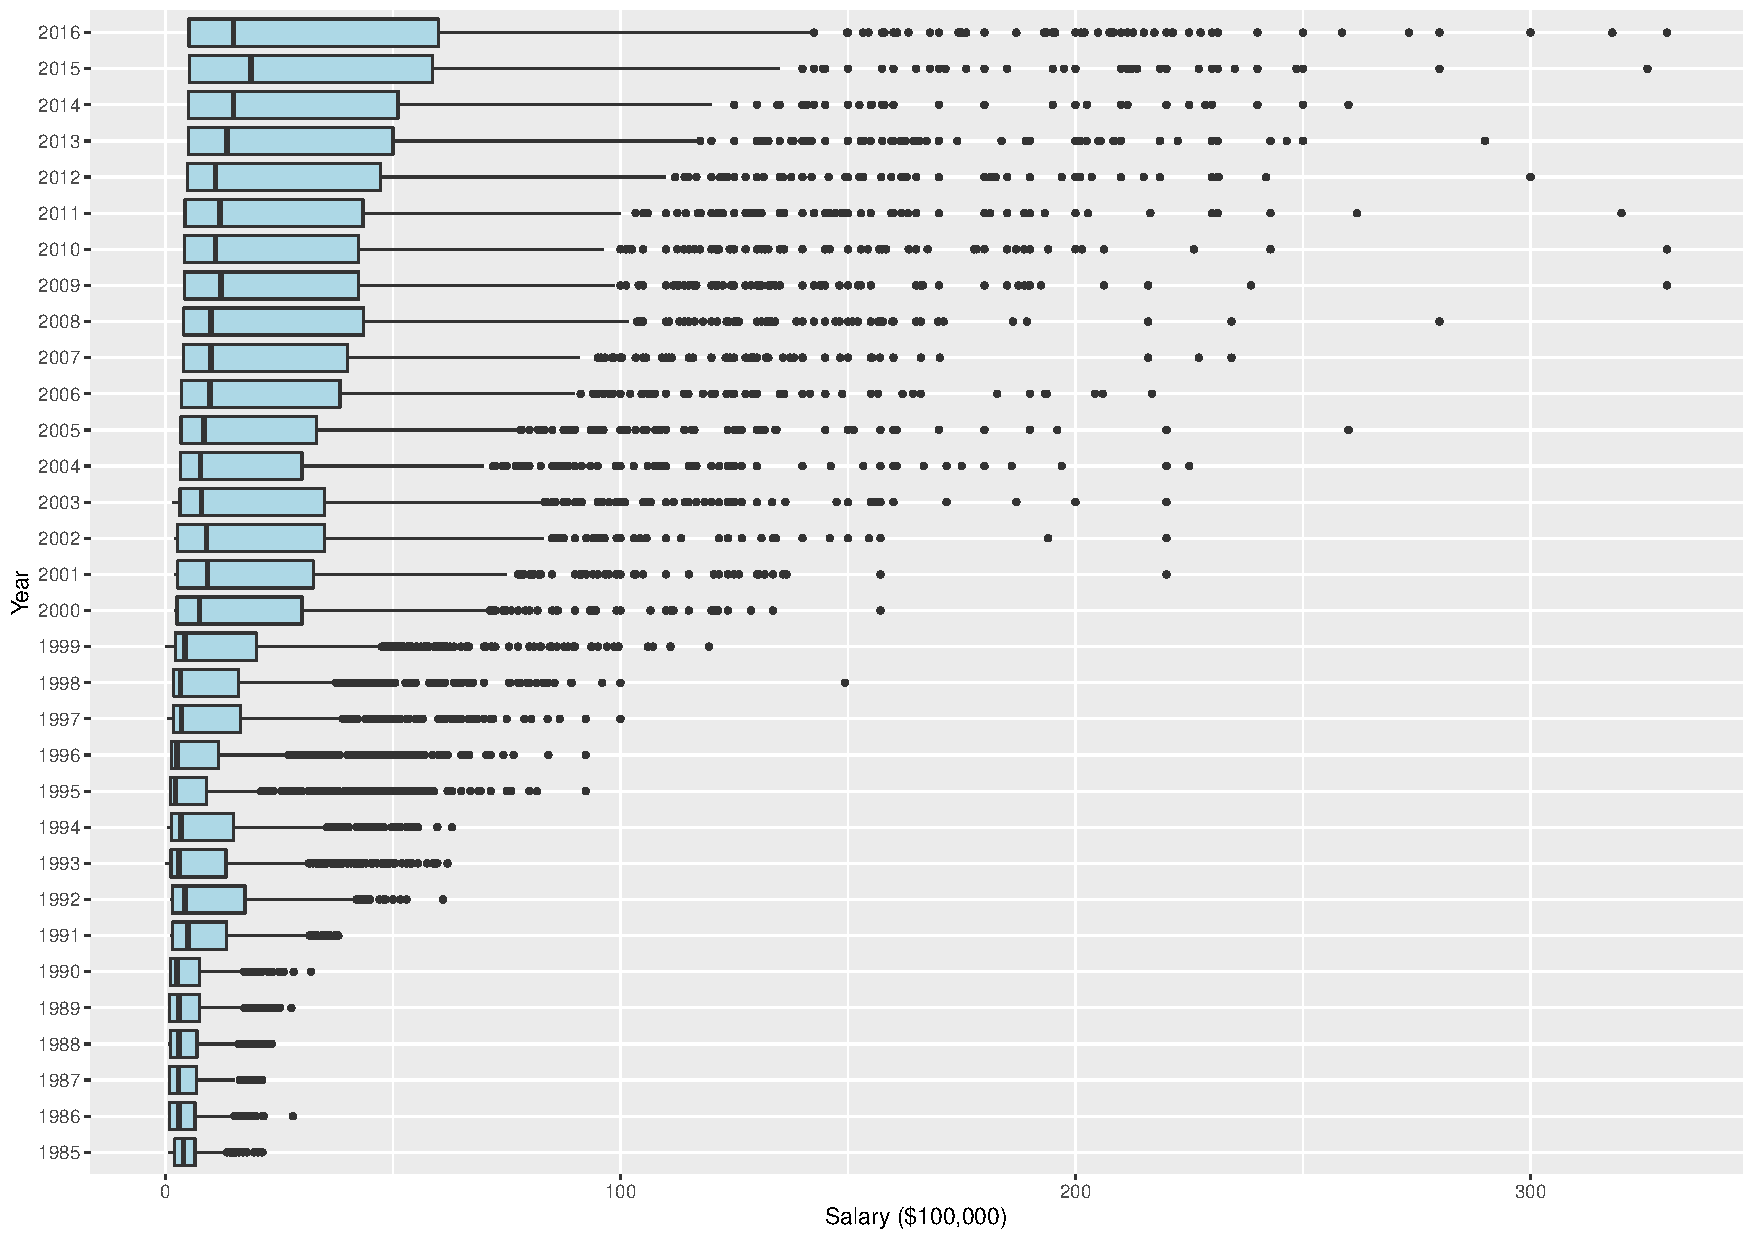
\includegraphics[width=10cm]{photographs/Salaries.pdf}
    \caption{Baseball Salaries over the years}
    \label{fig:Salary}
\end{figure}
We use data from 2010 to predict a players salary in 2011 given how well the player did. Here is the code to isolate the data:
\subsubsection{Training Data}
\begin{minted}[frame=single]{R}
batting <- Batting %>%
  filter(yearID == 2010) %>%
  left_join(select(Salaries, playerID, yearID, teamID, salary), 
            by=c("playerID", "yearID", "teamID"))
str(batting)

batting %>%
  filter(! is.na(salary))

names(batting)
salarybatting = subset(batting, select = -c(playerID, teamID, lgID))
salarybatting[is.na(salarybatting)] <- 0
\end{minted}

\subsubsection{Testing Data}
\begin{minted}[frame=single]{R}
nextyear <- Batting %>%
  filter(yearID == 2011) %>%
  left_join(select(Salaries, playerID, yearID, teamID, salary), 
            by=c("playerID", "yearID", "teamID"))
str(nextyear)

nextyear %>%
  filter(! is.na(salary))

names(nextyear)
salarynextyear = subset(nextyear, select = -c(playerID, teamID, lgID))
salarynextyear[is.na(salarynextyear)] <- 0
\end{minted}

\chapter{Model Creation Code}


\end{appendices}

\end{document}